% arara: pdflatex: { synctex: yes }
% arara: makeindex: { style: ctuthesis }
% arara: bibtex
% arara: pdflatex
% arara: pdflatex

% Předání volby [table] balíku xcolor (loadovaný ctuthesis), aby fungovala střídavá barva řádků v~longtable.
\PassOptionsToPackage{table}{xcolor}

\documentclass[twoside]{ctuthesis}

% enumitem: rozšířené možnosti formátování seznamů (např. style=nextline u description).
\usepackage{enumitem}

% longtable: dlouhé tabulky s automatickým zalomením přes více stran (matice trasovatelnosti FR).
\usepackage{longtable}

% pifont: Zapf Dingbats pro symbol pokrytí v~matici trasovatelnosti FR (plný kruh \ding{108}).
\usepackage{pifont}
\newcommand{\yes}{\ding{108}}

% TikZ pro vlastní schémata (architektura, ER diagram, repozitářová vrstva, sekvenční diagram pipeline).
\usepackage{tikz}
\usetikzlibrary{positioning,arrows.meta,shapes.geometric,fit,calc,backgrounds,shapes.multipart}

% =========================================================================
% LADITELNÝ PARAMETR: zaoblení rohů iOS screenshotů (zlomek šířky obrázku).
%   0.04 = jemné, 0.06 = střední, 0.08-0.10 = výrazné, 0.13 = iOS spec.
% Změnou této hodnoty se přepočte zaoblení u všech 25 snímků v dokumentu.
\newcommand{\screenshotRadius}{0.13}
% =========================================================================

% Makro \screenshot pro zaoblené iOS snímky obrazovek.
% Použití: \screenshot[width=0.42\textwidth]{figures/screens/Foo.png}
\newsavebox{\screenshotbox}
\newcommand{\screenshot}[2][width=\textwidth]{%
	\savebox{\screenshotbox}{\includegraphics[#1]{#2}}%
	\begin{tikzpicture}
		\path[clip, rounded corners=\screenshotRadius\wd\screenshotbox]
			(0,0) rectangle (\wd\screenshotbox, \ht\screenshotbox);
		\node[inner sep=0pt, outer sep=0pt, anchor=south west] at (0,0) {\usebox{\screenshotbox}};
	\end{tikzpicture}%
}

\ctusetup{
	preprint = \ctuverlog,
	mainlanguage = czech,
	otherlanguages = {english},
	title-czech = {Aplikace pro rozpoznávání potravin a sledování kalorického příjmu pomocí AI},
	title-english = {AI-Powered Food Recognition and Calorie Tracking Application},
	doctype = M,
	faculty = F3,
	department-czech = {Katedra počítačové grafiky a interakce},
	department-english = {Department of Computer Graphics and Interaction},
	author = {Bc. Jakub Sebastian Andráš},
	supervisor = {Ing. Ivo Malý, Ph.D.},
	fieldofstudy-czech = {Otevřená informatika},
	subfieldofstudy-czech = {Interakce člověka s počítačem},
	fieldofstudy-english = {Open Informatics},
	subfieldofstudy-english = {Human-Computer Interaction},
	keywords-czech = {umělá inteligence, rozpoznávání potravin, sledování kalorií, mobilní aplikace, Flutter, OpenAI},
	keywords-english = {artificial intelligence, food recognition, calorie tracking, mobile application, Flutter, OpenAI},
	day = 1,
	month = 5,
	year = 2026,
}

\ctuprocess

\addto\ctucaptionsczech{%
	\def\supervisorname{Vedoucí}%
	\def\subfieldofstudyname{Studijní program}%
}

% Drobná svislá mezera mezi odstavci pro lepší čitelnost dlouhého technického textu.
% 0.5\baselineskip = cca 7 bodů (polovina řádku), kombinováno s odsazením prvního řádku.
% Pro hutnější (čistě indentovaný) styl: zakomentovat. Pro vzdušnější: zvýšit na 1\baselineskip.
\setlength{\parskip}{0.5\baselineskip plus 0.2ex minus 0.2ex}

% Český abstrakt
\begin{abstract-czech}
	% TODO: Doplnit český abstrakt po dokončení dlouhodobého testování (sekce~\ref{sec:dlouhodobeTestovani}).
\end{abstract-czech}

% Anglický abstrakt
\begin{abstract-english}
	% TODO: Add English abstract once long-term testing is finalised (see~\ref{sec:dlouhodobeTestovani}).
\end{abstract-english}

% Poděkování
\begin{thanks}
	Rád bych poděkoval vedoucímu práce Ing. Ivu Malému, Ph.D. za odborné vedení, věcné připomínky a~ochotu pravidelně diskutovat průběh práce.
	Poděkování patří také všem respondentům uživatelské studie a~participantům uživatelského testování za jejich čas, otevřenost a~konstruktivní zpětnou vazbu, bez níž by návrhová a~evaluační část této práce nemohla vzniknout.
	Děkuji rovněž rodině a~blízkým za podporu během celého studia.
\end{thanks}

% Prohlášení
\begin{declaration}
	Prohlašuji, že jsem předloženou práci vypracoval samostatně a že jsem uvedl veškeré
	použité informační zdroje v souladu s Metodickým pokynem o dodržování etických
	principů při přípravě vysokoškolských závěrečných prací.

	V Praze, \ctufield{day}.~\monthinlanguage{title}~\ctufield{year}
\end{declaration}

\begin{document}

\maketitle

\chapter{Úvod}
\label{ch:uvod}

Udržování zdravého životního stylu a optimální tělesné kondice představuje klíčový aspekt moderního pojetí kvality života.
Tento význam je zdůrazněn nejen individuálními cíli, jako je zvýšení energie či osobní spokojenosti, ale také aktuálními zdravotními trendy populace.
Podle dostupných dat se Češi umisťují na čtvrtém místě v žebříčku evropských zemí z hlediska výskytu nadváhy a obezity.
Celkem 55,4~\% české populace má tělesnou hmotnost vyšší než doporučené normy.
Horší jsou pouze Řecko, Chorvatsko a Malta, kde tento podíl dosahuje až 59,6~\%~\cite{evropskaMapaObezity2019}.

Motivace k osvojování udržitelných stravovacích a pohybových návyků je proto více než aktuální a různorodá, a to od prevence civilizačních chorob až po snahu o zlepšení celkové fyzické kondice a životní pohody.
Dosažení těchto cílů však vyžaduje systematický a informovaný přístup, který přesahuje pouhé počáteční odhodlání a opírá se o vědecké poznatky o výživě, energetickém příjmu a výdeji, stejně jako o praktické nástroje pro monitorování a optimalizaci životního stylu.

Základním principem regulace tělesné hmotnosti je energetická bilance.
Tento koncept definuje vztah mezi kaloriemi přijatými ve stravě a energií, kterou tělo spotřebuje na svůj provoz a veškerou fyzickou aktivitu.
Ačkoliv je tato myšlenka ve své podstatě jednoduchá, její praktická aplikace naráží na řadu překážek.
Mnoho lidí své úsilí vzdává, protože manuální zaznamenávání stravy je vnímáno jako zdlouhavé a nepraktické pro každodenní použití.
Bez systematického přehledu se pak snadno uchylují k neefektivním dietním zkratkám, které nevedou k dlouhodobým výsledkům.

Moderní technologie nabízejí jedno z možných řešení těchto problémů.
Zejména mobilní aplikace se staly rozšířeným nástrojem, který dokáže uživatele provázet jejich snahou, poskytovat jim okamžitou zpětnou vazbu a uchovávat data potřebná pro kvalifikovaná rozhodnutí o jídelníčku a pohybové aktivitě.
Současně se rozvíjí oblast umělé inteligence a počítačového vidění, která umožňuje částečně automatizovat dosud manuální úlohy, například odhad složení jídla z fotografie.

Náplní této práce je prozkoumat potenciál nejnovějších pokroků v oblasti umělé inteligence pro zjednodušení sledování kalorického příjmu.
Hlavním cílem je navrhnout a částečně realizovat aplikaci, která využívá schopností pokročilých modelů umělé inteligence k automatické analýze jídla z fotografie, čímž odstraňuje část bariér spojených s ručním zapisováním a činí proces správy jídelníčku efektivnější a uživatelsky přijatelnější.

Dílčími cíli práce jsou provedení rešerše současné odborné literatury v oblasti digitálních nástrojů pro výživu a využití umělé inteligence v této doméně, dále analýza stávajících řešení na trhu, která umožní identifikovat silné a slabé stránky konkurence a definovat prostor pro inovaci.
Na tuto analýzu navazuje výběr vhodných technologií a nástrojů, které budou pro potřeby implementace dostatečně výkonné a zároveň prakticky použitelné.
Neméně důležitou fází práce je návrh softwarové architektury pro zajištění spolehlivého chodu a efektivní komunikace mezi jednotlivými komponentami systému a vytvoření přehledného a intuitivního uživatelského rozhraní.

Na úvodní kapitolu navazuje část věnovaná rešerši odborných zdrojů a existujících mobilních aplikací pro sledování stravy.
Ta vytváří kontext pro návrh vlastního řešení a umožňuje zasadit diskutovanou aplikaci do širšího rámce digitálního zdraví a výzkumu v oblasti výživy.

\chapter{Analýza}
\label{ch:analyza}

\section{Obezita, nadváha a význam sledování stravy}
\label{sec:obezita}

Obezita a nadváha patří mezi klíčové determinanty morbidity a mortality v rozvinutých i rozvojových zemích.
Dlouhodobě zvýšená tělesná hmotnost je spojena se zvýšeným rizikem kardiovaskulárních onemocnění, diabetu 2.~typu, některých nádorových onemocnění a zhoršenou kvalitou života.
Epidemiologická data Eurostatu (zjišťování EU-SILC, referenční rok 2022) ukazují, že Česká republika patří v~rámci Evropské unie k~zemím s~vyšším podílem obézních dospělých~\cite{eurostatBmi2022}.
Konkrétní hodnoty byly uvedeny v~kapitole~\ref{ch:uvod}.

\subsection{Index tělesné hmotnosti a jeho interpretace}
\label{subsec:bmi}

Základním orientačním ukazatelem pro posouzení tělesné hmotnosti je index tělesné hmotnosti (Body Mass Index, BMI).
BMI se vypočítá jako podíl tělesné hmotnosti v~kilogramech a druhé mocniny tělesné výšky v~metrech:

\begin{equation}
	\mathrm{BMI} = \frac{m}{h^{2}},
	\label{eq:bmi}
\end{equation}

\noindent kde $m$ je tělesná hmotnost v~kilogramech a $h$ tělesná výška v~metrech.
Na základě hodnoty BMI se rozlišují jednotlivé kategorie výživového stavu definované Světovou zdravotnickou organizací, které jsou shrnuty v~tabulce~\ref{tab:bmi}.

\begin{table}[ht]
	\centering
	\caption{Hodnoty BMI a jejich interpretace.}
	\label{tab:bmi}
	\begin{tabular}{ll}
		\toprule
		\textbf{BMI (kg/m\textsuperscript{2})} & \textbf{Kategorie} \\
		\midrule
		pod 18,5 & podváha \\
		18,5--24,9 & normální hmotnost \\
		25,0--29,9 & nadváha \\
		30,0--34,9 & obezita I.~stupně \\
		35,0--39,9 & obezita II.~stupně \\
		40,0 a více & obezita III.~stupně \\
		\bottomrule
	\end{tabular}
\end{table}

BMI je pro populační studie a rychlé screeningové hodnocení velmi užitečné, protože umožňuje jednoduché srovnání mezi jedinci i populacemi.
Současně má však významná omezení.
Nezohledňuje rozložení tuku v~těle, podíl svalové hmoty ani individuální rozdíly v~tělesném složení.
U sportovců nebo lidí s~vysokým podílem svalové hmoty může proto docházet k~systematické klasifikaci do nadváhy či obezity, ačkoli jejich zdravotní riziko tomu neodpovídá~\cite{theodorakis2025humanEnergyBalance}.
BMI by tak měl být v~klinické i praktické práci vnímán jako orientační ukazatel, který je vhodné doplnit dalšími měřeními (obvod pasu, složení těla, laboratorní ukazatele).

\subsection{Životní styl, energetická bilance a rozvoj obezity}
\label{subsec:zivotniStyl}

Současné konceptuální modely chápou obezitu jako dlouhodobý důsledek pozitivní energetické bilance, kdy energetický příjem převyšuje energetický výdej.
Theodorakis a~Nikolaou popisují, že do energetické bilance vstupuje řada vzájemně provázaných proměnných, například bazální metabolismus, termický efekt potravy, spontánní pohyb, strukturovaná fyzická aktivita a adaptivní metabolické změny~\cite{theodorakis2025humanEnergyBalance}.
To znamená, že dvě osoby se stejným kalorickým příjmem a podobnou tělesnou hmotností mohou mít odlišný dlouhodobý vývoj hmotnosti v~závislosti na rozdílech v~energetickém výdeji a hormonální regulaci.

Drenowatz a~Greier zdůrazňují, že efektivní řízení tělesné hmotnosti vyžaduje současnou práci se stravou i fyzickou aktivitou.
Izolované intervence zaměřené pouze na dietní omezení nebo pouze na cvičení dosahují obvykle menšího a hůře udržitelného efektu než integrované přístupy, které systematicky pracují s~oběma složkami energetické bilance~\cite{drenowatz2025integrating}.
Z~hlediska návrhu digitálních nástrojů je proto důležité uvažovat tělesnou hmotnost v~širším kontextu životního stylu, nikoli jen jako mechanický výsledek krátkodobého kalorického deficitu.

\section{Self monitoring jako nástroj řízení hmotnosti}
\label{sec:selfMonitoring}

Jedním z~klíčových behaviorálních principů používaných v~programech redukce hmotnosti je self monitoring, tedy systematické sledování vlastního chování.
V~oblasti výživy se self monitoring nejčastěji projevuje jako pravidelný záznam konzumovaných jídel, sledování tělesné hmotnosti a zaznamenávání fyzické aktivity.
Cílem je zvýšit povědomí o~vlastních návycích a umožnit uživateli, aby své chování průběžně upravoval v~souladu s~doporučeními.

Systematické přehledy ukazují, že pravidelný self monitoring příjmu potravy a tělesné hmotnosti je spojen s~větším úbytkem hmotnosti a lepším udržením dosažených změn než situace, kdy je sledování nepravidelné nebo zcela chybí.
Zároveň se ukazuje, že self monitoring lze realizovat různými způsoby od papírových deníků až po digitální nástroje a mobilní aplikace, přičemž forma záznamu ovlivňuje jak přesnost dat, tak dlouhodobou udržitelnost celého procesu.
Detailní přehled vybraných mobilních aplikací pro sledování stravy a jejich charakteristik je proto věnován samostatné podkapitole~\ref{sec:existujici}~\cite{ang2021efficacy,raber2021systematicReview}.

Souhrnně lze říci, že obezita a nadváha představují významný zdravotní problém v~České republice i celosvětově a že self monitoring patří mezi hlavní behaviorální nástroje pro redukci a udržení tělesné hmotnosti.
Jeho dlouhodobá účinnost je však omezená tím, že pravidelné zaznamenávání jídel a souvisejících údajů je časově i kognitivně náročné, což vede u~řady uživatelů k~postupnému poklesu frekvence záznamů a k~oslabení efektu jinak dobře nastavených intervencí.
Tento kontext vytváří přímou motivaci pro hledání nástrojů, které sníží zátěž spojenou se sledováním stravy a tím zvýší pravděpodobnost, že uživatelé budou nástroj využívat konzistentně i v~delším časovém horizontu~\cite{pujia2025roleMobileApps,crane2023patterns,theodorakis2025humanEnergyBalance}.

\section{Energetická bilance a nutriční základy}
\label{sec:energetickaBilance}

Pochopení principu energetické bilance je zásadní pro interpretaci výstupů z~každé aplikace, která pracuje s~kalorickým příjmem a výdejem.
Následující podkapitoly definují klíčové pojmy: energetickou hodnotu makroživin, složky celkového energetického výdeje, prediktivní rovnice pro odhad bazálního metabolismu, samotný vztah mezi příjmem a výdejem a zdroje chyb v~odhadu obou veličin.

\subsection{Kalorie a energetická hodnota potravin}
\label{subsec:kalorie}

V~nutriční praxi se jako jednotka energie používá kilokalorie (kcal), případně kilojoule (kJ).
Jedna kilokalorie odpovídá množství energie potřebné ke zvýšení teploty jednoho kilogramu vody o~jeden stupeň Celsia.
V~běžné komunikaci se pojem „kalorie" používá téměř vždy ve významu kilokalorie.
Energetická hodnota potravin vyjadřuje množství energie, které organismus může z~dané potraviny získat.
Základní makroživiny se liší i svou energetickou hodnotou.
Sacharidy a bílkoviny poskytují přibližně 4~kcal na gram, zatímco tuky zhruba 9~kcal na gram, tedy více než dvojnásobek~\cite{theodorakis2025humanEnergyBalance}.

Pro udržení tělesné hmotnosti v~rovnováze musí být dlouhodobě energetický příjem z~potravin v~rovnováze s~energetickým výdejem.
Systematické odchylky v~podobě chronického kalorického deficitu nebo nadbytku vedou k~postupné změně tělesné hmotnosti~\cite{theodorakis2025humanEnergyBalance}.

\subsection{Složky energetického výdeje}
\label{subsec:slozkyVydeje}

Celkový denní energetický výdej (TEE) se obvykle rozděluje na několik složek:

\begin{itemize}
	\item bazální metabolismus (BMR),
	\item termický efekt potravy (TEF),
	\item energetický výdej na fyzickou aktivitu, který zahrnuje jak strukturované cvičení, tak běžný denní pohyb.
\end{itemize}

Theodorakis a~Nikolaou uvádějí, že u~většiny dospělé populace tvoří bazální metabolismus přibližně 60 až 75~\% celkového energetického výdeje.
Zbývající část připadá na termický efekt potravy a fyzickou aktivitu, přičemž jejich relativní význam se může výrazně lišit v~závislosti na životním stylu~\cite{theodorakis2025humanEnergyBalance}.

Bazální metabolismus představuje množství energie, které organismus potřebuje v~klidových podmínkách pro udržení základních životních funkcí, jako je činnost srdce a plic, udržování tělesné teploty a syntéza tkání.
Je ovlivněn především:

\begin{itemize}
	\item množstvím a složením tělesné hmoty (zejména podílem beztukové hmoty),
	\item věkem,
	\item pohlavím,
	\item genetickými faktory a hormonálním stavem.
\end{itemize}

\subsection{Prediktivní rovnice pro odhad bazálního metabolismu}
\label{subsec:bmrRovnice}

Přímé měření energetického výdeje pomocí nepřímé kalorimetrie není v~běžné praxi ani v~uživatelských aplikacích reálně dostupné.
Místo něj se využívají empirické prediktivní rovnice odhadující BMR ze snadno měřitelných parametrů (hmotnost, výška, věk, pohlaví).
Historicky nejrozšířenější je Harris-Benedictova rovnice z~roku 1919, novější Mifflin-St~Jeorova rovnice z~roku 1990 však bývá řadou novějších studií hodnocena jako přesnější pro běžnou dospělou populaci~\cite{frankenfield2005comparison} a má tvar:

\begin{align}
	\mathrm{BMR}_{\text{muži}} &= (10 \cdot m) + (6{,}25 \cdot h) - (5 \cdot a) + 5,   \label{eq:msj-muzi} \\
	\mathrm{BMR}_{\text{ženy}} &= (10 \cdot m) + (6{,}25 \cdot h) - (5 \cdot a) - 161, \label{eq:msj-zeny}
\end{align}

\noindent kde $m$ je hmotnost v~kilogramech, $h$ výška v~centimetrech a $a$ věk v~letech.
Systematické přehledy zároveň ukazují, že přesnost prediktivních rovnic se liší mezi populacemi a u~některých skupin (zejména sportovci a lidé s~nadprůměrným podílem svalové hmoty) mohou běžně používané rovnice BMR systematicky podhodnocovat nebo nadhodnocovat~\cite{frankenfield2005comparison}.
V~uživatelských aplikacích je proto použití těchto rovnic praktickým kompromisem mezi dostupností dat a požadavkem na rychlý odhad energetického výdeje, doprovázeným srozumitelnou komunikací nejistoty výsledku směrem k~uživateli.

\subsection{Energetická bilance a energetická nerovnováha}
\label{subsec:nerovnovaha}

Energetickou bilanci lze zjednodušeně vyjádřit rovnicí:

\begin{equation}
	\Delta E_{\text{zásoby}} = E_{\text{příjem}} - E_{\text{výdej}}.
	\label{eq:bilance}
\end{equation}

Pokud je energetický příjem dlouhodobě nižší než energetický výdej, organismus čerpá chybějící energii z~uložených zásob, především z~tukové tkáně.
Tento stav se označuje jako kalorický deficit a vede k~postupnému snižování tělesné hmotnosti.
Příliš výrazný a dlouhodobý deficit však může kromě tukové tkáně ohrožovat i svalovou hmotu a vést k~nedostatku živin, únavě a zhoršení zdravotního stavu~\cite{theodorakis2025humanEnergyBalance,drenowatz2025integrating}.

Naopak při chronickém kalorickém nadbytku převyšuje energetický příjem výdej.
Přebytečná energie se ukládá ve formě tukových zásob a dochází k~postupnému zvyšování tělesné hmotnosti a rizika metabolických onemocnění.
Drenowatz a~Greier zdůrazňují, že významnou roli hraje nejen absolutní množství energie, ale také struktura stravy, rozložení příjmu během dne a míra fyzické aktivity.
Účinné strategie řízení hmotnosti proto kombinují dietní úpravy s~podporou pohybové aktivity~\cite{drenowatz2025integrating}.

\subsection{Zdroje chyb v~odhadu příjmu a výdeje energie}
\label{subsec:zdrojeChyb}

Praktické využití energetické bilance v~každodenním životě naráží na zásadní problém, kterým je nepřesnost odhadů jak na straně příjmu, tak na straně výdeje.
Uživatelé běžně podhodnocují množství a energetickou hodnotu zkonzumovaných potravin, zapomínají zaznamenávat některá jídla nebo špatně odhadují velikost porcí.
Li a~kol. například prokázali, že výstupy nutričních aplikací se mohou významně lišit od referenčních metod, a to jak při manuálním zapisování, tak při využití rozpoznávání obrazu~\cite{li2024evaluating}.

Na straně energetického výdeje může docházet k~nadhodnocování spálené energie, zejména pokud uživatel spoléhá na obecné tabulky nebo méně přesná zařízení.
Theodorakis a~Nikolaou upozorňují, že organismus navíc na energetický deficit adaptivně reaguje snížením bazálního metabolismu a spontánního pohybu, což dále komplikuje přesnou predikci změn tělesné hmotnosti~\cite{theodorakis2025humanEnergyBalance}.

Pro návrh digitálního nástroje to znamená, že:

\begin{itemize}
	\item nelze spoléhat na absolutní přesnost jednoho konkrétního čísla energetického příjmu nebo výdeje,
	\item je vhodné pracovat s~konceptem odhadu s~nejistotou,
	\item design rozhraní by měl uživatele motivovat ke konzistentnímu zapisování a zároveň usilovat o~minimalizaci zátěže.
\end{itemize}

Právě tato snaha o~snížení uživatelské zátěže při zachování dostatečné přesnosti odhadu energetické bilance je jedním z~hlavních důvodů, proč tato práce zkoumá možnosti využití umělé inteligence a rozpoznávání potravin z~fotografie.

\section{Makroživiny a mikroživiny ve výživě}
\label{sec:zivoiny}

Při hodnocení kvality stravy je vedle celkového energetického příjmu zásadní také její složení.
To určují především makroživiny, které dodávají energii a stavební materiál, a mikroživiny, jež umožňují správný průběh metabolických a regulačních procesů.
Přehledové studie ukazují, že jak poměr makroživin, tak dostatečný příjem klíčových mikroživin mají významný vliv na tělesné zdraví, riziko chronických onemocnění i subjektivní pohodu~\cite{venn2020macronutrients,farag2021dietaryMicronutrients}.

\subsection{Makroživiny}
\label{subsec:makrozivny}

Makroživiny tvoří hlavní zdroj energie ve stravě a zahrnují sacharidy, tuky a bílkoviny.
Sacharidy (jednoduché cukry, škrob, vláknina) jsou primárním zdrojem energie pro většinu buněk, přičemž strava s~vyšším zastoupením komplexních sacharidů a vlákniny je spojována s~lepší kontrolou glykemie a vyšším pocitem sytosti.
Tuky představují koncentrovaný zdroj energie a jsou nezbytné pro vstřebávání lipofilních vitamínů.
Významnou roli hraje jejich kvalitativní složení, neboť vyšší podíl nenasycených mastných kyselin je spojován s~příznivým vlivem na kardiovaskulární zdraví~\cite{venn2020macronutrients}.
Bílkoviny jsou základním stavebním materiálem tkání a hormonů, přičemž jejich dostatečný příjem je klíčový zejména pro udržení svalové hmoty při redukci tělesné hmotnosti~\cite{venn2020macronutrients}.

Z~praktického hlediska je vedle celkového energetického příjmu důležitá i kvalita jednotlivých makroživin a dlouhodobá udržitelnost stravovacího režimu, protože různé dietní přístupy mohou vést ke srovnatelným změnám hmotnosti, pokud je zachován celkový energetický deficit~\cite{theodorakis2025humanEnergyBalance,drenowatz2025integrating}.

\subsection{Mikroživiny}
\label{subsec:mikrozivny}

Mikroživiny (vitaminy a minerální látky) na rozdíl od makroživin nepřinášejí významné množství energie, ale podílejí se na enzymatických a regulačních procesech v~organismu a jejich nedostatek může ovlivnit imunitu, kognitivní funkce i riziko chronických onemocnění~\cite{farag2021dietaryMicronutrients}.
V~aktuální verzi navrhované aplikace se sledování mikroživin neuvažuje, neboť přesahuje rámec primárního cíle, kterým je snížení bariéry kalorického záznamu.
Jejich začlenění je však relevantním kandidátem pro budoucí rozšíření aplikace o~kvalitativní hodnocení stravy, zejména v~kontextu fenoménu \uv{skryté malnutrice}, kdy vysoký energetický příjem může být doprovázen nedostatečným příjmem některých mikroživin~\cite{farag2021dietaryMicronutrients}.

\section{Existující mobilní aplikace pro sledování stravy}
\label{sec:existujici}

Mobilní aplikace pro sledování stravy a tělesné hmotnosti patří v~současnosti k~nejčastěji používaným nástrojům digitálního zdraví a přehledové studie potvrzují jejich přínos pro lepší kontrolu stravovacích návyků a mírnou redukci hmotnosti~\cite{nogueira2024mobileApplications}.
Systematické průzkumy hlavních mobilních obchodů identifikují v~této kategorii stovky vzájemně konkurujících aplikací, například Samad a~kol. nalezli 473 aplikací souvisejících se sledováním příjmu potravy, z~nichž 80 podrobně analyzovali~\cite{samad2022smartphoneApps,abeltino2025digitalApplications}.

Přehledy výživových aplikací ukazují, že většina z~nich staví na velmi podobném jádru a liší se spíše v~uživatelském rozhraní a doplňkových funkcích než v~samotné logice sledování stravy~\cite{nogueira2024mobileApplications,abeltino2025digitalApplications}.
Společné jádro typicky zahrnuje potravinový deník, databázi potravin s~fulltextovým vyhledáváním, ukládání vlastních receptů a oblíbených jídel, nastavení cílového energetického příjmu a základní vizualizaci výsledků formou grafů a statistik~\cite{gioia2023mobileApps}.
Z~hlediska zadávání dat většina komerčních aplikací nadále spoléhá na manuální zapisování doplněné o~částečně automatizované zkratky, zejména skenování čárových kódů, šablony jídel s~možností duplikace dříve zapsaných záznamů a připomenutí ve formě notifikací~\cite{abeltino2025digitalApplications}.
Empirickou oporu pro popis silných a slabých stránek této kategorie aplikací poskytuje analýza Zečević a~kol., kteří metodou \emph{topic modelingu} zpracovali 72\,084 recenzí z~Google Play Store pro patnáct nejpoužívanějších aplikací pro sledování stravy a identifikovali jedenáct opakujících se témat~\cite{zecevic2021userPerspectives}.
Mezi nejhůře hodnocené patří netransparentní účtování předplatného (průměrné hodnocení 2,32 z~5) a technická stabilita (2,85 z~5), zatímco kladně jsou vnímány jednoduchost ovládání, samotná funkce zápisu kalorií a integrace čtečky čárových kódů~\cite{zecevic2021userPerspectives}.

Systematické studie zároveň upozorňují, že ruční zapisování je časově náročné a v~praxi často vede k~nekompletním či zkresleným záznamům.
Li a~kol. ukazují, že výstupy nutričních aplikací se mohou od referenčních metod významně lišit jak u~manuálního zapisování, tak u~řešení s~podporou rozpoznání obrazu, přičemž energetický příjem bývá podle typu stravy nadhodnocen nebo podhodnocen o~stovky kilokalorií denně~\cite{li2024evaluating}.
V~reakci na tato omezení se prosazuje využití umělé inteligence a počítačového vidění, avšak Samad a~kol. ve svém vzorku 80 aplikací identifikovali pouze jedinou, která dokázala z~fotografie automaticky určit druh jídla i velikost porce~\cite{samad2022smartphoneApps}.
Aburub a~kol. shrnují, že plně automatické rozpoznávání talíře zůstává výjimkou a typicky vyžaduje potvrzení a korekci uživatele, zatímco skenování čárových kódů se mezitím stalo běžným standardem~\cite{aburub2025foodScanning}.

Chotwanvirat a~kol. ve své rešerši 84 prací publikovaných do roku 2021 dokumentují, že po roce 2015 vystřídaly ruční extrakci příznaků konvoluční neuronové sítě překračující 80~\% přesnosti na datasetech FOOD-101 a UEC FOOD-256~\cite{chotwanvirat2024scoping}.
Tatáž rešerše upozorňuje, že většina takto trénovaných systémů zůstává omezena na curated datasety, hůře se vyrovnává s~reálnými podmínkami snímání a postrádá vysvětlitelnost svých rozhodnutí, což ztěžuje jejich přijetí v~klinické praxi~\cite{chotwanvirat2024scoping}.
Liu a~kol. tento závěr kvantifikují i na novější transformerové architektuře CBiAFormer, jejíž přesnost klesá z~92,40~\% na západním datasetu ETHZ Food-101 na 72,92~\% na smíšeném ISIA Food-200, což ilustruje obecnější obtíž specializovaných modelů zobecnit napříč kuchyněmi~\cite{liu2025deepLearning}.

Po roce 2022 nastupuje v~oboru třetí vlna v~podobě multimodálních velkých jazykových modelů, které dokáží v~jediném volání zpracovat obraz, text i hlasový přepis a vrátit strukturovaný odhad nutričních hodnot bez nutnosti vlastního trénování na potravinovém datasetu~\cite{wang2026visionLanguageFood,fridolfsson2025llmNutrition}.
Recentní studie a preprinty z~let 2025 a 2026 ukazují, že tyto modely při vhodném prompt engineeringu dosahují srovnatelné nebo lepší přesnosti odhadu kalorické hodnoty než dříve nasazované specializované sítě~\cite{hua2025nutribench,coburn2025multimodalNutrition}.
Tento posun zároveň přesouvá těžiště přesnosti z~architektury a tréninkových dat směrem k~designu promptu a postprocessingu odpovědi modelu, čemuž je v~rámci této práce věnována experimentální validace popsaná v~kapitole~\ref{ch:testovani}~\cite{ase2025structuredPrompts}.

Pro tuto práci jsou reprezentativní čtyři aplikace, které lze rozdělit do dvou typologicky odlišných skupin.
První skupinu tvoří tradiční aplikace s~manuálním potravinovým deníkem, v~němž umělá inteligence funguje jako asistent rychlejšího zápisu, zastoupené globálním MyFitnessPal a československými Kalorickými Tabulkami (Dine4Fit).
Druhou skupinu tvoří novější aplikace stavící primárně na rozpoznávání jídla z~fotografie, ilustrované americkým SnapCalorie a novějším komerčním zástupcem této vlny CalZen.
Toto rozdělení odráží rozdíl mezi etablovaným ekosystémem deníkových aplikací a komerčním projevem třetí vlny popsané výše, jejíž jádro tvoří multimodální modely nasazené po roce 2022~\cite{wang2026visionLanguageFood,fridolfsson2025llmNutrition}.
Následující podsekce obě skupiny stručně představují a vymezují jejich silné a slabé stránky ve vztahu k~cíli této diplomové práce.

\subsection{Tradiční aplikace s~manuálním zápisem}
\label{subsec:tradicniAplikace}

Tato skupina představuje dlouhodobě dominantní jádro trhu, na němž stojí drtivá většina z~více než čtyř stovek aplikací identifikovaných systematickými průzkumy hlavních mobilních obchodů~\cite{samad2022smartphoneApps,abeltino2025digitalApplications}.
Jejím společným rysem je strukturovaný potravinový deník navázaný na rozsáhlou databázi potravin a zápis založený především na manuálním vyhledávání, doplněný o~částečně automatizované zkratky typu skenování čárových kódů, šablon jídel a foto rozpoznávání~\cite{abeltino2025digitalApplications,gioia2023mobileApps}.
Pro tuto skupinu je charakteristické, že umělá inteligence vstupuje až jako sekundární funkce nad existujícím deníkovým rozhraním, nikoli jako primární vstupní kanál~\cite{aburub2025foodScanning}.

\subsubsection{MyFitnessPal}
\label{subsubsec:myfitnesspal}

MyFitnessPal patří mezi nejznámější a nejrozšířenější aplikace pro sledování stravy a tělesné hmotnosti na světě, je dostupný pro Android, iOS i webové rozhraní a dlouhodobě se pohybuje na předních příčkách kategorií Health \& Fitness v~hlavních mobilních obchodech~\cite{myFitnessPal2025}.
Základem aplikace je potravinový deník navázaný na rozsáhlou databázi potravin obsahující miliony položek včetně značkových výrobků a restaurací.
Uživatel zapisuje jídla vyhledáváním v~databázi, výběrem z~historie, skenováním čárového kódu nebo zadáním vlastních receptů.
Aplikace průběžně počítá denní energetický příjem a rozložení makroživin, podporuje záznam fyzických aktivit, sledování hmotnosti a integraci s~externími zařízeními (Apple Health, fitness náramky).
Pokročilé funkce, jako je sledování mikronutrientů a detailnější nutriční přehledy, jsou součástí placeného předplatného Premium~\cite{myFitnessPal2025}.

MyFitnessPal je jedním z~prvních velkých komerčních produktů, které nasadily ve větším měřítku foto rozpoznávání jídel.
Funkce Meal Scan umožňuje uživateli namířit fotoaparát na talíř, přičemž aplikace pomocí počítačového vidění navrhne odpovídající položky a velikosti porcí z~interní databáze, které uživatel potvrdí nebo upraví~\cite{myFitnessPal2025}.
Klíčovými přednostmi z~hlediska této práce jsou rozsáhlá globální databáze, kombinace více vstupních metod a dlouhodobá přítomnost na trhu doložená nezávislými studiemi~\cite{samad2022smartphoneApps}.
Mezi omezeními naopak figuruje proměnlivá kvalita uživatelsky přidaných položek vedoucí k~chybám v~nutričních údajích, nutnost ruční kontroly výsledků foto rozpoznávání~\cite{li2024evaluating} a nedostatečné pokrytí lokálních středoevropských produktů.
MyFitnessPal je tak referenčním příkladem robustního ekosystému, který umělou inteligenci využívá primárně jako doplněk manuálního zápisu, nikoli jako jeho plnou náhradu.

\subsubsection{Kalorické Tabulky}
\label{subsubsec:kalorickeTabulky}

Kalorické Tabulky, vyvíjené společností Dine4Fit~a.s., představují nejpoužívanější aplikaci pro sledování stravy v~českém a slovenském prostředí.
Podle oficiálních údajů firmy ji měsíčně používá více než jeden milion uživatelů~\cite{dine4fit2025}.
Aplikace je dostupná jako web i mobilní aplikace pro Android a iOS a podporuje vybrané chytré hodinky (Garmin, Apple Watch).
Její základní princip se podobá globálním nástrojům: potravinový deník navázaný na databázi výrazně přizpůsobenou regionálnímu trhu, sledování pitného režimu a hmotnosti, záznam fyzických aktivit a kalorická kalkulačka odvozující doporučený příjem z~tělesných parametrů a cílů uživatele~\cite{dine4fit2025}.
Stejně jako MyFitnessPal funguje aplikace ve freemium modelu, kde rozšířené analýzy, mikronutrienty a pokročilé statistiky jsou součástí placeného Premium~\cite{dine4fit2025}.

Novější verze Kalorických Tabulek integrují funkci rozpoznávání jídel z~fotografie pomocí umělé inteligence: uživatel jídlo vyfotí a aplikace navrhne odpovídající potraviny a přibližnou gramáž~\cite{dine4fit2025}.
Stejně jako u~MyFitnessPal nejde o~plně autonomní systém, nezávislá kvantitativní studie přesnosti této konkrétní funkce v~recenzované literatuře zatím chybí, což odpovídá obecnějšímu trendu opožděné akademické validace komerčních AI funkcí~\cite{samad2022smartphoneApps,li2024evaluating,aburub2025foodScanning}.
Hlavními přednostmi v~českém kontextu jsou silná lokalizace databáze, dostupnost webového i mobilního rozhraní a velká uživatelská základna přispívající ke komunitním receptům~\cite{dine4fit2025}.
Mezi limity patří časová náročnost při práci se složitějšími recepty, riziko nepřesností v~komunitně rozšiřovaných databázích~\cite{li2024evaluating} a stále spíše doplňková role AI rozpoznávání vůči manuálnímu zápisu.

\subsection{Aplikace stavící primárně na AI rozpoznávání}
\label{subsec:aiFirstAplikace}

Skupina se vnitřně dělí na dva přístupy, které jsou v~následujících podkapitolách reprezentovány aplikacemi SnapCalorie a CalZen, totiž vlastní specializovaný model trénovaný na uceleném potravinovém datasetu a generický multimodální model nasazený přes API~\cite{coburn2025multimodalNutrition}.

\subsubsection{SnapCalorie}
\label{subsubsec:snapcalorie}

Aplikace SnapCalorie je vyvíjena americkým týmem, jehož zakladatelé pocházejí z~výzkumu počítačového vidění ve společnosti Google a podle veřejných materiálů firmy se podíleli na vzniku produktů Google Lens a Cloud Vision API~\cite{snapcalorie2025}.
Technologickým jádrem je vlastní specializovaný model trénovaný na proprietárním datasetu zhruba 5\,000 jídel, jejichž ingredience byly před fotografováním na robotickém rigu zváženy na laboratorní váze~\cite{snapcalorie2025}.
Cílem této koncepce je pokrýt obtížné případy typu polévek, mixovaných pokrmů a omáček, na kterých generické datasety selhávají~\cite{snapcalorie2025,chotwanvirat2024scoping}.
Doprovodnou výbavou je databáze přibližně 500\,000 položek validovaná oproti referenčnímu zdroji USDA, skener nutričních štítků a integrace s~platformou Apple HealthKit, přičemž každý odhad lze ručně upravit a model je deklarován jako učící se z~uživatelských korekcí~\cite{snapcalorie2025}.

Sebereportovaná průměrná chyba odhadu energetické hodnoty činí podle vyjádření výrobce přibližně 15~\%, což je v~publikovaných materiálech srovnáváno s~tolerancí 20~\% povolenou na nutričních štítcích a s~vyššími chybovostmi nutričních specialistů a běžných uživatelů konkurenčních aplikací~\cite{snapcalorie2025}.
Tyto údaje pocházejí výhradně od provozovatele a v~recenzované literatuře k~nim zatím chybí nezávislá validační studie, což odpovídá obecnějšímu jevu opožděné akademické verifikace komerčních AI funkcí~\cite{samad2022smartphoneApps,li2024evaluating,aburub2025foodScanning}.
Z~hlediska této práce je SnapCalorie referenčním příkladem \emph{AI-first} přístupu se specializovaným vlastním modelem, jehož hlavními limity jsou převážně západní složení trénovacího datasetu, slabá lokalizace mimo Spojené státy a obtížnější přenositelnost do prostředí české a středoevropské kuchyně, kterou kvantifikuje pokles přesnosti specializovaných sítí napříč regionálními datasety~\cite{liu2025deepLearning}.

\subsubsection{CalZen}
\label{subsubsec:calzen}

Aplikace CalZen reprezentuje generickou vlnu AI-first nástrojů uvedených v~letech 2024 a 2025, které slibují odhad kalorické a makroživinové hodnoty z~fotografie pokrmu řádově do několika sekund a podle vyjádření provozovatele rozpoznají domácí jídla, restaurační pokrmy i balené potraviny~\cite{calzen2025}.
Provozovatel deklaruje řádově tři miliony uživatelů a průměrné hodnocení 4,8~z~5 v~hlavních mobilních obchodech, jedná se však o~marketingové údaje výrobce bez nezávislé verifikace~\cite{calzen2025}.
Doprovodné funkce zahrnují krokoměr a sledování pitného režimu a aplikace funguje ve freemium modelu, v~němž jsou pokročilé makroanalýzy a integrace dostupné v~placeném tarifu~\cite{calzen2025}.

Na rozdíl od SnapCalorie firma technické řešení blíže nedokumentuje a nezveřejňuje, jaký model rozpoznávání používá ani jakou metodikou je měřena přesnost odhadu~\cite{calzen2025}.
Krátký inferenční čas a generická šíře pokrývající různorodé kuchyně, restaurace i obalová balení jsou konzistentní s~nasazením multimodálních velkých jazykových modelů přes API, jak je dokumentuje recentní literatura~\cite{wang2026visionLanguageFood,fridolfsson2025llmNutrition,coburn2025multimodalNutrition}.
Pro tuto práci je CalZen typovým představitelem druhého přístupu v~rámci AI-first skupiny, tedy generického multimodálního modelu nasazeného bez vlastního trénování, jehož silnou stránkou je rychlost vývoje a šíře pokrytí, slabinami pak nízká technická transparentnost, absence veřejné validační studie a slabé pokrytí české kuchyně srovnatelné s~limity SnapCalorie~\cite{li2024evaluating,aburub2025foodScanning}.

\subsection{Shrnutí aplikací na trhu}
\label{subsec:shrnutiTrhu}

Čtyři představené aplikace ilustrují dvě paralelní vlny současného trhu se sledováním stravy, totiž tradiční deníkové nástroje s~rozsáhlými databázemi a milionovými uživatelskými základnami na straně jedné a AI-first aplikace stavící foto rozpoznávání jako primární vstup na straně druhé~\cite{abeltino2025digitalApplications,wang2026visionLanguageFood}.
Druhá skupina není inovací posledních měsíců, ale několikaletým komerčním trendem, který v~návaznosti na multimodální modely uvedené po roce 2022 už generuje uživatelské základny v~řádu milionů, jak dokládají sebereportované údaje aplikací typu SnapCalorie a CalZen~\cite{snapcalorie2025,calzen2025,fridolfsson2025llmNutrition}.
Společným rysem obou skupin však zůstává, že nezávislá akademická validace přesnosti komerčních AI funkcí v~recenzované literatuře nadále chybí, a to jak u~doplňkového foto rozpoznávání v~tradičních aplikacích typu MyFitnessPal Meal Scan, tak u~plně AI-first řešení~\cite{samad2022smartphoneApps,li2024evaluating,aburub2025foodScanning}.

Pozici této diplomové práce v~uvedeném kontextu nevymezuje ambice překonat komerční AI-first nástroje v~technické přesnosti rozpoznávání, ke které by autorský tým bez zdrojů firem typu SnapCalorie neměl reálné prostředky.
Diferenciace je postavena na třech osách, které ani jedna z~představených aplikací nepokrývá současně, totiž na lokalizované databázi potravin postavené na evropském zdroji Open Food Facts s~důrazem na regionální produkty, na transparentním zobrazení nejistoty AI výstupu uživateli a na integraci s~evropským zdravotním ekosystémem prostřednictvím Apple Health a Health Connect~\cite{dine4fit2025,liu2025deepLearning}.
Tato kombinace odpovídá identifikovaným slabinám trhu, na nichž zaostává jak globální MyFitnessPal v~lokalizaci, tak SnapCalorie a CalZen v~pokrytí české kuchyně i v~transparentnosti komunikace omezení modelu~\cite{zecevic2021userPerspectives,liu2025deepLearning}.

Z~uvedeného přehledu vyplývají pro návrh aplikace v~této diplomové práci tři hlavní závěry, které jsou konzistentní i s~kvantitativní analýzou nejčastějších stížností uživatelů ve studii Zečević a~kol.~\cite{zecevic2021userPerspectives}.
Za prvé, inovace by neměla cílit na samotnou existenci AI funkce, která je již na trhu komoditou, ale na konkrétní slabá místa stávajících řešení, zejména na uživatelskou zátěž zápisu, kvalitu lokální databáze a transparentní komunikaci nejistoty výstupu vůči uživateli~\cite{zecevic2021userPerspectives,li2024evaluating}.
Za druhé, AI-first přístup je dostupný i bez vlastního trénovaného modelu skrze multimodální velké jazykové modely nasazené přes API, což otevírá prostor pro rychlou implementaci v~rámci diplomové práce~\cite{wang2026visionLanguageFood}.
Za třetí, lokální kontext, podpora české a středoevropské kuchyně a kvalitní lokalizovaná databáze zůstávají diferenciátorem i vůči AI-first konkurenci typu SnapCalorie a CalZen, která je primárně orientovaná na západní a anglosaský trh~\cite{liu2025deepLearning,dine4fit2025}.

\section{Uživatelská studie}
\label{sec:uzivatelskaStudie}

Uživatelská studie představuje soubor metod, jejichž cílem je porozumět potřebám, motivacím a kontextu cílových uživatelů a tyto poznatky následně převést do návrhu systému.
V~oblasti mobilního zdraví je uživatelsky orientovaný přístup považován za důležitý, protože ovlivňuje použitelnost, důvěru, dlouhodobou adherenci a tím i reálný dopad aplikace~\cite{cornet2020untoldStories}.

V~této práci byla uživatelská studie použita jako hlavní vstup pro návrh aplikace pro rozpoznávání potravin pomocí umělé inteligence a pro sledování kalorického příjmu.
Cílem bylo identifikovat situace, ve kterých je ruční zapisování pro uživatele překážkou, jaká míra nepřesnosti je akceptovatelná, jak uživatelé vnímají selhání umělé inteligence a jaké podpůrné funkce zvyšují pravděpodobnost dlouhodobého používání.

Účastníci uživatelské studie jsou v~textu označováni \texttt{R1}--\texttt{R4} (Respondent rozhovorů) a tvoří odlišnou skupinu od participantů \texttt{P1}--\texttt{P3} v~kapitole~\ref{ch:testovani}, která referuje samostatné uživatelské testování implementované aplikace.

\subsection{Metodika}
\label{subsec:metodika}

Jako metoda sběru dat byly zvoleny strukturované rozhovory s~uživateli z~cílové skupiny.
Rozhovory byly vedeny tak, aby pokryly současnou praxi zapisování jídel, očekávání od rozpoznávání pomocí umělé inteligence a také preference v~oblasti přehledů, motivace, práce s~daty a integrací.
Tento postup odpovídá doporučením v~literatuře, kde jsou kvalitativní techniky typu rozhovorů nebo skupinových diskusí uváděny jako vhodný zdroj požadavků pro návrh aplikací v~oblasti zdraví~\cite{molina2020proposalUserCentered}.

Rozhovory byly zpracovány do samostatných reportů a dále analyzovány tematickým způsobem.
V~této kapitole jsou výsledky shrnuty do hlavních témat, která následně tvoří vstup pro formalizaci scénářů případů užití a sady funkčních a nefunkčních požadavků v~kapitole~\ref{ch:navrh}.
Reporty v~plném znění jsou součástí příloh této práce.

\subsection{Charakteristika respondentů}
\label{subsec:participanti}

Pro rozhovory byli vybráni čtyři respondenti, kteří reprezentují rozdílné cíle a kontext používání.
V~textu jsou uváděni anonymizovaně jako R1 až R4.

\begin{description}
	\item[R1] muž ve věku 27~let, jehož cílem je nabírání svalové hmoty.
		Cvičí přibližně třikrát týdně a preferuje sledování makroživin.
		V~minulosti aplikaci pro zapisování využíval, ale přestal, když dosáhl cíle.
		Je ochoten tolerovat určitou míru nepřesnosti, pokud mu aplikace ušetří práci.
	\item[R2] muž ve věku 24~let, intenzivně cvičí a cíleně udržuje kalorický nadbytek.
		U~zapisování klade důraz na přesnost a důvěryhodnost, preferuje rychlé metody zadávání u~balených potravin, typicky čárové kódy.
		U~jídel z~restaurace akceptuje typicky vyšší nepřesnost při zápisu než u~jiných pokrmů.
	\item[R3] žena ve věku 54~let, dlouhodobě se snaží zhubnout a zohledňuje zdravotní souvislosti.
		Zkoušela existující aplikace, ale odradila ji časová náročnost, časté chybění položek v~databázi a nutnost odhadovat gramáž, zejména u~domácího vaření.
	\item[R4] žena ve věku 28~let, která dříve své jídlo pravidelně vážila, nyní častěji zapisuje odhadem a upřednostňuje jednoduché předvolby porcí.
		Má jasnou preferenci, aby fotografie byla primárním vstupem, ale současně požaduje kvalitní záložní cestu při selhání.
		Zásadní je pro ni transparentnost umělé inteligence a rozlišení běžných limitů modelu od technické chyby aplikace.
\end{description}

\subsection{Výsledky rozhovorů}
\label{subsec:vysledkyRozhovoru}

\paragraph{Rychlost zápisu a dlouhodobá udržitelnost.}
Opakovaným tématem napříč rozhovory je, že dlouhodobé používání je přímo podmíněno rychlostí a jednoduchostí.
R1 zmiňuje cílový stav rychlého zápisu jednoduché položky přibližně do šesti kliknutí bez dodatečné editace.
R2 uvádí podobnou hranici pro rychlé položky.
R4 toleruje pomalejší zpracování zejména na začátku, ale očekává postupné zrychlení a udržení zápisu v~přiměřeném čase.
Zcela klíčové je to pro R3, která pomalost procesu zápisu označila za hlavní důvod, proč v~dosavadních pokusech přestávala aplikaci používat ještě před dosažením svých zdravotních cílů.

\paragraph{Akceptovatelná nepřesnost a důvěra v~umělou inteligenci.}
Respondenti se liší v~toleranci nepřesnosti, což je klíčové pro definici cílových metrik přesnosti.
R1 je ochoten tolerovat přibližnou odchylku do dvaceti procent, pokud mu aplikace výrazně zjednoduší proces.
Naopak R2 požaduje nepřesnost pouze v~řádu jednotek procent a bez důvěryhodného výsledku považuje funkci za málo užitečnou.
R3 chápe omezení vysoké přesnosti, nicméně požaduje, aby výstup byl srozumitelný a kontrolovatelný, zejména u~domácích jídel.

\paragraph{Selhání rozpoznání.}
Pro praktickou použitelnost funkce rozpoznávání je kritické eliminovat situace, kdy se uživatel ocitne ve slepé uličce.
R4 požaduje, aby při selhání fotografie bylo možné plynule přejít na textový popis a aby bylo možné rozpoznání znovu vyvolat z~rozpracovaného záznamu bez zakládání nového záznamu.
R1 zároveň navrhuje možnost doplnit k~fotografii krátkou doplňující informaci pro lepší výsledek.
Důležitým aspektem je také rozlišení, zda jde o~limit rozpoznání, nebo o~technickou chybu aplikace, a nabídnutí vhodného dalšího kroku.

\paragraph{Oblíbená jídla, historie a zkratky.}
Všichni respondenti popisují situace, kdy jedí opakovaně podobná jídla, případně používají stejné ingredience.
R2 označuje oblíbené položky, historii a čtečku kódů za zásadní funkce.
R4 uvádí, že využívá oblíbené a duplikaci předešlého záznamu a ocení našeptávání dříve zadaných názvů.
R1 doplňuje potřebu rychlých zkratek, které umožní udržet zápis v~nízkém počtu kroků.

\paragraph{Domácí vaření a odhad množství.}
Domácí vaření se ukazuje jako jeden z~možných důvodů, proč uživatelé zapisování opouštějí.
R3 popisuje, že vaření od oka ztěžuje odhad gramáže a že největší bariéra nastává, když položka chybí v~databázi a je nutné ji vytvořit manuálně.
R2 zdůrazňuje potřebu práce s~plánovanými ingrediencemi a následnou jednoduchou úpravou skutečně použitých množství, včetně drobných ingrediencí typu olej nebo koření.
To vede k~požadavku na funkcionalitu, která podporuje plánování a následné rychlé dorovnání skutečně použitých množství surovin.

\paragraph{Kategorie jídel a práce se zpětným zápisem.}
Respondenti se liší v~tom, zda zapisují před jídlem nebo zpětně.
R2 u~jídel z~restaurace preferuje doplnění až doma mimo sociální situaci.
R3 uvádí, že zapisovala i večer, případně plánovala dopředu, ale nedodržení plánů vedlo ke zdvojení práce.
Z~toho vyplývá potřeba podporovat jak okamžitý zápis, tak zpětný zápis z~galerie, a zároveň nevnucovat automatické zařazování kategorií podle času zadání.

\paragraph{Přehledy, motivace a dotazování nad daty.}
Základem je pro všechny denní přehled, tedy rychlá kontrola kalorií a makroživin.
R1 požaduje jednoduché přehledy po dnech, týdnech a měsících a možnost pokládat dotazy typu porovnání období podle makroživin.
R4 vnímá týdenní souhrn jako užitečné doplnění a navrhuje dotazování přirozeným jazykem s~personalizovanými doporučeními.
R2 uvádí, že motivační měsíční souhrny formou notifikace nebo e-mailu by mu pomohly udržet rutinu.
R3 klade důraz na dietní omezení a schopnost odpovědět, kolikrát došlo k~porušení diety s~proklikem na konkrétní dny.

\paragraph{Soukromí, ukládání dat a kontrola.}
Otázka soukromí se objevuje ve smyslu kontroly nad daty a transparentností práce s~nimi.
R1 požaduje jasné funkce pro mazání a informace o~tom, co se s~daty děje.
R4 je ochotna akceptovat automatické promazávání nejstarších záznamů mimo oblíbené položky.
R3 považuje za důležité mít možnost smazat jednotlivé záznamy, i když je pro ni umístění dat méně podstatné.

\paragraph{Integrace aktivity.}
Integrace se sportovními službami a hodinkami se opakuje u~všech respondentů, byť s~rozdílnou hloubkou.
R1 chce jednoduché propojení a zobrazení příjmu versus výdeje.
R2 očekává přebírání spálených kalorií s~možností nastavit, zda a jak se výdej promítne do denního limitu.
R4 zmiňuje zájem o~integraci s~Garmin a zdůrazňuje, že ji zajímá zejména promítnutí spálených kalorií do denního přehledu.

\subsection{Shrnutí kapitoly}
\label{subsec:shrnutiUS}

Uživatelská studie ukázala, že hlavní bariérou dlouhodobého zapisování je kombinace časové náročnosti, nejistoty výsledků a slabé podpory pro opakované situace, zejména opakovaná jídla, balené produkty, domácí vaření a pokrmy z~restaurací.
Rozpoznávání pomocí umělé inteligence je vnímáno jako přínosné, ale pouze za předpokladu, že uživatel má kontrolu nad výsledkem a rozumí nejistotě spojené s~vyhodnocením.
Výstupy rozhovorů byly formulovány do scénářů případů užití a do sady požadavků, které tvoří přímý podklad pro návrh a realizaci prototypu v~kapitole~\ref{ch:navrh}.

\chapter{Návrh aplikace}
\label{ch:navrh}

% TODO: úvodní odstavec, který stručně nastíní nadcházející kapitoly v Návrhu aplikace,
% což bude Existující řešení, Uživatelská studie (strukturované rozhovory),
% z nich vyplynou Use cases, FR/NFR, případy užití,
% a na jejichž základě bude zkonstruován HiFi prototyp aplikace.

\section{Existující řešení}
\label{sec:existujici}

Mobilní aplikace pro sledování stravy a tělesné hmotnosti patří v~současnosti k~nejčastěji používaným nástrojům v~oblasti digitálního zdraví.
Přehledové studie ukazují, že nutriční a dietní aplikace jsou běžnou součástí změny životního stylu a mohou přispět k~lepší kontrole stravovacích návyků a k~mírné redukci hmotnosti~\cite{nogueira2024mobileApplications}.

Současné analýzy trhu s~digitálními nástroji pro výživu potvrzují, že v~hlavních mobilních obchodech existují desítky až stovky aplikací zaměřených na sledování příjmu potravy, plánování jídelníčku a takzvanou precision nutrition.
Abeltino a~kol. ve svém přehledu shrnují, že pro běžné uživatele i odborníky je k~dispozici široké spektrum aplikací pro monitorování stravy a tvorbu jídelních plánů~\cite{abeltino2025digitalApplications}.
Samad a~kol. při systematickém průzkumu tří velkých obchodů s~aplikacemi identifikovali 473 aplikací souvisejících se sledováním příjmu potravy a doporučováním jídel, z~nichž 80 podrobně analyzovali~\cite{samad2022smartphoneApps}.
To dokládá, že i v~jedné poměrně úzce vymezené kategorii existují desítky až stovky vzájemně konkurujících aplikací.

Přehledy výživových aplikací ukazují, že většina z~nich staví na velmi podobném jádru a liší se spíše v~uživatelském rozhraní a doplňkových funkcích než v~samotné logice sledování stravy~\cite{nogueira2024mobileApplications,abeltino2025digitalApplications}.
Typická aplikace pro sledování stravy nabízí zejména:

\begin{itemize}
	\item potravinový deník pro každodenní záznam jídel,
	\item databázi potravin s~nutričními hodnotami a fulltextovým vyhledáváním,
	\item možnost ukládat vlastní recepty a oblíbená jídla,
	\item nastavení cílového energetického příjmu a sledování makroživin,
	\item základní zpětnou vazbu ve formě grafů a statistik~\cite{gioia2023mobileApps}.
\end{itemize}

Z~hlediska interakce s~uživatelem je klíčové zadávání dat.
Většina komerčních aplikací stále vyžaduje manuální zapisování jídel prostřednictvím vyhledávání v~databázi nebo zadávání receptů.
Částečnou automatizaci přinášejí:

\begin{itemize}
	\item skenování čárových kódů balených potravin,
	\item předvyplněné šablony jídel a možnost kopírovat dříve zapsaná jídla,
	\item notifikace připomínající záznam jednotlivých jídel~\cite{abeltino2025digitalApplications}.
\end{itemize}

Systematické studie zároveň upozorňují, že ruční zapisování je časově náročné a v~praxi často vede k~nekompletním či zkresleným záznamům.
Li a~kol. ukazují, že výstupy nutričních aplikací se mohou od referenčních metod významně lišit, a to jak u~manuálního zapisování, tak u~řešení s~podporou rozpoznání obrazu.
Energetický příjem bývá v~závislosti na typu stravy nadhodnocen nebo podhodnocen o~stovky kilodžaulů až kilokalorií denně~\cite{li2024evaluating}.

V~reakci na omezení manuálního sběru dat se začíná prosazovat využití umělé inteligence a počítačového vidění.
Samad a~kol. ukazují, že pouze malá část komerčních aplikací nabízí pokročilé funkce automatického rozpoznávání jídel z~fotografie a odhadu porce, a že v~souboru 80 hodnocených aplikací byla jen jedna, která dokázala z~fotografie automaticky určit druh jídla i velikost porce~\cite{samad2022smartphoneApps}.
Aburub a~kol. ve svém přehledu food scanning aplikací shrnují, že skenování čárových kódů je dnes běžnou funkcí, zatímco plně automatické rozpoznávání talíře zůstává výjimkou a typicky vyžaduje potvrzení a korekci ze strany uživatele~\cite{aburub2025foodScanning}.

Nogueira-Rio a~kol. zdůrazňují, že současná generace výživových aplikací stojí na kombinaci tradičního self monitoringu a nových AI nástrojů, přičemž zásadní výzvou je skloubit vyšší míru automatizace s~přijatelnou přesností a použitelností v~každodenním životě~\cite{nogueira2024mobileApplications}.

Pro tuto práci jsou reprezentativní zejména dvě aplikace, které pokrývají globální i lokální kontext.
První je mezinárodní aplikace MyFitnessPal a druhou jsou československé Kalorické Tabulky (Dine4Fit).
Následující podkapitoly je stručně představují a vymezují jejich silné a slabé stránky ve vztahu k~cíli této diplomové práce.

\subsection{MyFitnessPal}
\label{subsec:myfitnesspal}

MyFitnessPal patří mezi nejznámější a nejrozšířenější aplikace pro sledování stravy a tělesné hmotnosti na světě.
Je dostupná pro Android, iOS i webové rozhraní a dlouhodobě se pohybuje na předních příčkách kategorií Health \& Fitness v~hlavních mobilních obchodech~\cite{myFitnessPal2025}.

\subsubsection*{Hlavní funkcionalita}

Základem MyFitnessPal je potravinový deník navázaný na rozsáhlou databázi potravin.
Oficiální materiály uvádějí databázi s~miliony položek včetně běžných potravin, značkových výrobků i restaurací.
Uživatel může zapisovat jídelníček několika způsoby:

\begin{itemize}
	\item vyhledáváním v~databázi podle názvu potraviny,
	\item výběrem z~historie a často používaných jídel,
	\item skenováním čárového kódu u~balených potravin,
	\item zadáváním vlastních receptů a pokrmů.
\end{itemize}

Aplikace průběžně počítá celkový denní energetický příjem a zobrazuje rozložení makroživin, jako jsou sacharidy, tuky a bílkoviny.
V~placené verzi umožňuje sledovat i další nutriční parametry, například vlákninu, cukr, sůl nebo vybrané mikronutrienty.
Součástí systému je také záznam fyzických aktivit, sledování tělesné hmotnosti a integrace s~externími zařízeními a službami, jako jsou Apple Health nebo fitness náramky~\cite{myFitnessPal2025}.

Obchodní model aplikace odpovídá freemium přístupu.
Základní funkce potravinového deníku a databáze potravin jsou dostupné zdarma, rozšířené analytické nástroje, pokročilé nastavení cílů, detailnější nutriční přehledy a některé zrychlené způsoby zadávání jídel jsou součástí placeného předplatného MyFitnessPal Premium~\cite{myFitnessPal2025}.

\subsubsection*{Rozpoznávání jídel z~fotografie}

MyFitnessPal je jedním z~prvních velkých komerčních produktů, které nasadily ve větším měřítku foto rozpoznávání jídel.
Funkce Meal Scan umožňuje uživateli namířit fotoaparát na talíř a aplikace na základě obrazu navrhne odpovídající položky z~databáze.
Podle oficiální dokumentace jde o~funkci dostupnou v~rámci předplatného Premium a aktuálně podporovanou pro vybrané verze iOS a Androidu~\cite{myFitnessPal2025}.

Výrobce uvádí, že Meal Scan využívá metody počítačového vidění a strojového učení k~identifikaci více položek na jednom talíři a jejich propojení s~interní databází.
V~praxi funguje Meal Scan jako asistovaná funkce: uživatel dostane seznam odpovídajících jídel, zvolí nejbližší položku a případně upraví velikost porce~\cite{myFitnessPal2025}.

\subsubsection*{Silné stránky a omezení}

Z~hlediska této práce jsou klíčové následující výhody MyFitnessPal:

\begin{itemize}
	\item rozsáhlá databáze potravin pokrývající globální trh, včetně restaurací a značkových výrobků~\cite{myFitnessPal2025},
	\item kombinace více vstupních metod (vyhledávání, historie, čárový kód, foto rozpoznávání)~\cite{myFitnessPal2025},
	\item dlouhodobá přítomnost na trhu, díky níž existuje řada nezávislých hodnocení této kategorie nástrojů, včetně studií zaměřených na kvalitu a funkce aplikací pro sledování stravy~\cite{samad2022smartphoneApps}.
\end{itemize}

Současná literatura i uživatelské zkušenosti ale upozorňují na několik omezení:

\begin{itemize}
	\item část databáze tvoří uživateli přidané položky, což může vést k~chybám v~nutričních údajích a nutnosti ruční korekce, například po skenování čárového kódu~\cite{li2024evaluating},
	\item i přes použití foto rozpoznávání zůstává nutnost ruční kontroly a úprav, zejména u~složitějších jídel a kombinovaných receptů~\cite{li2024evaluating},
	\item aplikace je navržena primárně pro globální trh, a proto nemusí dostatečně pokrývat některé lokální produkty nebo značky, zejména ve středoevropském kontextu.
\end{itemize}

Pro návrh vlastního řešení je MyFitnessPal důležitým referenčním příkladem robustního ekosystému, který kombinuje manuální self monitoring s~prvky umělé inteligence.
Současně ukazuje, že i jedna z~nejrozšířenějších aplikací využívá umělou inteligenci primárně jako doplněk, nikoli jako plnou náhradu manuálního zadávání.

\subsection{Kalorické Tabulky}
\label{subsec:kalorickeTabulky}

Kalorické Tabulky, vyvíjené společností Dine4Fit~a.s., představují nejpoužívanější aplikaci pro sledování stravy v~českém a slovenském prostředí.
Podle oficiálních informací firmy se stala nejpopulárnější aplikací na hlídání stravy v~Česku i na Slovensku a měsíčně ji používá více než jeden milion uživatelů~\cite{dine4fit2025}.
Tyto údaje potvrzuje také nezávislá reportáž na serveru CzechCrunch, která uvádí více než 1,5~milionu aktivních uživatelů a několik milionů registrací~\cite{houska2024kalorickeTabulky}.

Aplikace je dostupná na webu i jako mobilní aplikace pro Android a iOS a podporuje také vybrané chytré hodinky, například Garmin nebo Apple Watch~\cite{dine4fit2025}.

\subsubsection*{Hlavní funkcionalita}

Základní princip Kalorických Tabulek se podobá globálním aplikacím pro sledování stravy, je však výrazně přizpůsoben specifikům českého a slovenského trhu.
Klíčové funkce jsou:

\begin{itemize}
	\item databáze potravin zaměřená na produkty dostupné v~Česku a na Slovensku, včetně značkových výrobků, restaurací a uživatelských receptů~\cite{dine4fit2025},
	\item potravinový deník s~možností zapisovat jednotlivá jídla v~průběhu dne a sledovat energetický příjem v~kcal nebo kJ,
	\item přehled denního příjmu a výdeje energie, sledování pitného režimu a tělesné hmotnosti~\cite{dine4fit2025},
	\item podpora záznamu fyzických aktivit a jejich vlivu na energetickou bilanci.
\end{itemize}

Významnou součástí ekosystému je i kalorická kalkulačka, která odvozuje doporučený energetický příjem z~tělesných parametrů a cílů uživatele.
Dine4Fit uvádí, že nastavení poměru makroživin vychází z~odborných doporučení a umožňuje zvolit různé cíle, jako je udržení hmotnosti, hubnutí nebo nárůst svalové hmoty~\cite{dine4fit2025}.

Aplikace používá freemium model.
Základní funkcionalita, tedy deník, výpočet energie a základní nutriční hodnoty, je dostupná zdarma, zatímco detailnější analýzy, rozšířené sledování mikronutrientů, speciální jídelníčky a pokročilé statistiky jsou součástí placeného předplatného Premium~\cite{dine4fit2025,houska2024kalorickeTabulky}.

\subsubsection*{Rozpoznávání jídel z~fotografie}

Novější verze Kalorických Tabulek integrují funkci rozpoznávání jídel z~fotografie pomocí umělé inteligence.
Podle popisu aplikace v~Google Play může uživatel jídlo vyfotit a aplikace navrhne odpovídající potraviny a jejich přibližnou gramáž, čímž automaticky spočítá kalorie a živiny~\cite{dine4fit2025}.
Dine4Fit tuto funkci dále popisuje na svém webu a blogu jako prémiovou novinku využívající umělou inteligenci pro rozpoznání jídel a odhad hmotnosti na základě fotografie~\cite{dine4fit2025}.

Technologické detaily implementace nejsou veřejně detailně popsány, mediální články nicméně zmiňují, že aplikace využívá detekci potravin pomocí umělé inteligence ve velkém objemu zaznamenaných jídel a že funkce je nasazována postupně s~důrazem na praktické využití v~běžném hubnutí~\cite{houska2024kalorickeTabulky}.

Stejně jako u~MyFitnessPal nejde o~plně autonomní systém.
Uživatelé musí výsledek zkontrolovat, případně upravit typ jídla nebo velikost porce.
Odborná literatura zatím neobsahuje nezávislou kvantitativní studii přesnosti této konkrétní funkce, což odpovídá obecnějšímu trendu, kdy detailní vědecká validace komerčních AI funkcí obvykle následuje s~časovým odstupem za jejich praktickým nasazením~\cite{samad2022smartphoneApps,li2024evaluating,aburub2025foodScanning}.

\subsubsection*{Silné stránky a omezení}

V~českém a slovenském kontextu mají Kalorické Tabulky několik výrazných výhod:

\begin{itemize}
	\item silná lokalizace databáze potravin na regionální produkty, včetně běžných značek a lokálních jídel~\cite{dine4fit2025},
	\item dostupnost webového rozhraní i mobilních aplikací, což usnadňuje zapisování v~různých situacích~\cite{dine4fit2025},
	\item velká uživatelská základna, která přispívá k~rozšiřování databáze a komunitním receptům~\cite{houska2024kalorickeTabulky}.
\end{itemize}

Současně však z~uživatelských recenzí a odborných diskusí vyplývá několik slabších míst relevantních pro návrh této práce:

\begin{itemize}
	\item práce se složitějšími recepty může být časově náročná a vyžaduje manuální sestavování položek,
	\item podobně jako u~jiných komunitně rozšiřovaných databází se mohou vyskytnout chyby v~nutričních údajích, pokud uživatelé zadávají data nepřesně~\cite{li2024evaluating},
	\item funkce rozpoznávání jídel pomocí umělé inteligence je relativně nová a dostupné informace ji popisují jako doplněk k~tradičnímu zadávání, nikoli jako plnou náhradu manuálního zápisu~\cite{dine4fit2025,houska2024kalorickeTabulky}.
\end{itemize}

Pro navrhovanou aplikaci jsou Kalorické Tabulky cenným vzorem z~hlediska lokalizace, práce s~regionálně specifickou databází a integrace funkcí umělé inteligence do jinak klasického stravovacího deníku.

\subsection{Shrnutí aplikací na trhu}
\label{subsec:shrnutiTrhu}

Odborná literatura a analýzy komerčního trhu ukazují, že výživové a dietní aplikace tvoří velmi početnou a relativně homogenní kategorii digitálních nástrojů.
Přehledy trhu a analýzy obchodů s~aplikacemi naznačují, že v~globálním měřítku existují desítky až stovky aplikací zaměřených na sledování stravy, které si vzájemně konkurují v~rámci několika málo funkčních podkategorií, například calorie tracker, nutrition tracker, diet planner nebo food scanning aplikace~\cite{abeltino2025digitalApplications,samad2022smartphoneApps}.

Samad a~kol. identifikovali 473 aplikací souvisejících s~příjmem potravy a doporučováním jídel a 80 z~nich podrobili detailnímu hodnocení~\cite{samad2022smartphoneApps}.
Gioia a~kol. pak ve svém přehledu vybrali reprezentativní soubor dietních aplikací a analyzovali jejich funkcionalitu a vhodnost pro výzkum stravovacích návyků~\cite{gioia2023mobileApps}.
Přestože se metodiky liší, obě práce ukazují, že ve sledované kategorii se vyskytují desítky až stovky aplikací, které sdílejí velmi podobnou základní funkcionalitu.

Napříč těmito aplikacemi se opakují zejména tyto prvky:

\begin{itemize}
	\item potravinový deník pro každodenní záznam jídel,
	\item databáze potravin s~nutričními hodnotami,
	\item ruční nebo poloautomatické zadávání pomocí čárového kódu a šablon,
	\item přehledy o~denním příjmu energie a makroživin, někdy doplněné o~motivační prvky a připomenutí,
	\item napojení na sledování tělesné hmotnosti a často i na fyzickou aktivitu~\cite{abeltino2025digitalApplications,gioia2023mobileApps}.
\end{itemize}

Rozdíly mezi jednotlivými aplikacemi se proto často týkají spíše míry propracovanosti uživatelského rozhraní a motivace, kvality a lokalizace potravinové databáze, míry integrace s~nositelnou elektronikou a rozsahu využití umělé inteligence pro automatizaci záznamu~\cite{nogueira2024mobileApplications,abeltino2025digitalApplications}.

Studie zaměřené na přesnost a uživatelskou zátěž potvrzují, že ruční zapisování stravy je pro mnoho lidí dlouhodobě obtížné a že dietní aplikace mohou energetický příjem podhodnocovat nebo nadhodnocovat, někdy i o~stovky kilokalorií denně~\cite{li2024evaluating}.
To vytváří prostor pro inovace v~oblasti automatizace sběru dat, především prostřednictvím obrazového rozpoznávání a dalších metod umělé inteligence.
Současně však scoping a systematické přehledy upozorňují, že plně automatické foto rozpoznávání je zatím spíše výjimkou a že i pokročilé funkce vyžadují aktivní roli uživatele~\cite{samad2022smartphoneApps,aburub2025foodScanning}.

MyFitnessPal a Kalorické Tabulky představují dva výrazné příklady této situace.
Na jedné straně ukazují vyspělost trhu, tedy rozsáhlé databáze, škálu vstupních metod, robustní ekosystém a milionové uživatelské základny~\cite{myFitnessPal2025,dine4fit2025,houska2024kalorickeTabulky}.
Na straně druhé potvrzují, že základní model zůstává obdobný jako v~počátcích mobilních dietních aplikací.
Uživatel stále primárně ručně zapisuje jídla do deníku a funkce foto rozpoznávání slouží jako doplněk, nikoli jako plná náhrada manuálního sběru dat~\cite{li2024evaluating,aburub2025foodScanning}.

Pro návrh aplikace v~této diplomové práci z~toho vyplývají tři hlavní závěry:

\begin{enumerate}
	\item Trh již nabízí velké množství aplikací se srovnatelnou základní funkcionalitou, takže inovace by měla cílit na konkrétní slabá místa, například uživatelskou zátěž při zadávání nebo kvalitu a lokalizaci databáze.
	\item Zvýšení míry automatizace pomocí počítačového vidění a umělé inteligence je slibnou cestou, ale vyžaduje pečlivé řešení otázky přesnosti a transparentní komunikaci nejistot vůči uživateli.
	\item Lokální kontext a kvalita potravinové databáze mohou být v~českém prostředí stejně důležité jako samotná technická vyspělost modelu rozpoznávání.
\end{enumerate}

\section{Uživatelská studie}
\label{sec:uzivatelskaStudie}

Uživatelská studie představuje soubor metod, jejichž cílem je porozumět potřebám, motivacím a kontextu cílových uživatelů a tyto poznatky následně převést do návrhu systému.
V~oblasti mobilního zdraví je uživatelsky orientovaný přístup považován za důležitý, protože ovlivňuje použitelnost, důvěru, dlouhodobou adherenci a tím i reálný dopad aplikace~\cite{cornet2020untoldStories}.

V~této práci byla uživatelská studie použita jako hlavní vstup pro návrh aplikace pro rozpoznávání potravin pomocí umělé inteligence a pro sledování kalorického příjmu.
Cílem bylo identifikovat situace, ve kterých je ruční zapisování pro uživatele překážkou, jaká míra nepřesnosti je akceptovatelná, jak uživatelé vnímají selhání umělé inteligence a jaké podpůrné funkce zvyšují pravděpodobnost dlouhodobého používání.

\subsection{Metodika}
\label{subsec:metodika}

Jako metoda sběru dat byly zvoleny strukturované rozhovory s~uživateli z~cílové skupiny.
Rozhovory byly vedeny tak, aby pokryly současnou praxi zapisování jídel, očekávání od rozpoznávání pomocí umělé inteligence a také preference v~oblasti přehledů, motivace, práce s~daty a integrací.
Tento postup odpovídá doporučením v~literatuře, kde jsou kvalitativní techniky typu rozhovorů nebo skupinových diskusí uváděny jako vhodný zdroj požadavků pro návrh aplikací v~oblasti zdraví~\cite{molina2020proposalUserCentered}.

Rozhovory byly zpracovány do samostatných reportů a dále analyzovány tematickým způsobem.
V~této kapitole jsou výsledky shrnuty do hlavních témat a následně formalizovány do scénářů případů užití a do sady funkčních a nefunkčních požadavků.
Reporty v~plném znění jsou součástí příloh této práce.

\subsection{Charakteristika participantů}
\label{subsec:participanti}

Pro rozhovory byli vybráni čtyři participanti, kteří reprezentují rozdílné cíle a kontext používání.
V~textu jsou uváděni anonymizovaně jako P1 až P4.

\begin{description}
	\item[P1] muž ve věku 27~let, jehož cílem je nabírání svalové hmoty.
		Cvičí přibližně třikrát týdně a preferuje sledování makroživin.
		V~minulosti aplikaci pro zapisování využíval, ale přestal, když dosáhl cíle.
		Je ochoten tolerovat určitou míru nepřesnosti, pokud mu aplikace ušetří práci.
	\item[P2] muž ve věku 24~let, intenzivně cvičí a cíleně udržuje kalorický nadbytek.
		U~zapisování klade důraz na přesnost a důvěryhodnost, preferuje rychlé metody zadávání u~balených potravin, typicky čárové kódy.
		U~jídel z~restaurace akceptuje typicky vyšší nepřesnost při zápisu než u~jiných pokrmů.
	\item[P3] žena ve věku 54~let, dlouhodobě se snaží zhubnout a zohledňuje zdravotní souvislosti.
		Zkoušela existující aplikace, ale odradila ji časová náročnost, časté chybění položek v~databázi a nutnost odhadovat gramáž, zejména u~domácího vaření.
	\item[P4] žena ve věku 28~let, která dříve své jídlo pravidelně vážila, nyní častěji zapisuje odhadem a upřednostňuje jednoduché předvolby porcí.
		Má jasnou preferenci, aby fotografie byla primárním vstupem, ale současně požaduje kvalitní záložní cestu při selhání.
		Zásadní je pro ni transparentnost umělé inteligence a rozlišení běžných limitů modelu od technické chyby aplikace.
\end{description}

\subsection{Výsledky rozhovorů}
\label{subsec:vysledkyRozhovoru}

\paragraph{Rychlost zápisu a dlouhodobá udržitelnost.}
Opakovaným tématem napříč rozhovory je, že dlouhodobé používání je přímo podmíněno rychlostí a jednoduchostí.
P1 zmiňuje cílový stav rychlého zápisu jednoduché položky přibližně do šesti kliknutí bez dodatečné editace.
P2 uvádí podobnou hranici pro rychlé položky.
P4 toleruje pomalejší zpracování zejména na začátku, ale očekává postupné zrychlení a udržení zápisu v~přiměřeném čase.
Zcela klíčové je to pro P3, která z~důvodů pomalosti procesu zápisu pokaždé přestala aplikaci používat, a to ještě před dosažením svých zdravotních cílů.

\paragraph{Akceptovatelná nepřesnost a důvěra v~umělou inteligenci.}
Participanti se liší v~toleranci nepřesnosti, což je klíčové pro definici cílových metrik přesnosti.
P1 je ochoten tolerovat přibližnou odchylku do dvaceti procent, pokud mu aplikace výrazně zjednoduší proces.
Naopak P2 požaduje nepřesnost pouze v~řádu jednotek procent a bez důvěryhodného výsledku považuje funkci za málo užitečnou.
P3 chápe omezení vysoké přesnosti, nicméně požaduje, aby výstup byl srozumitelný a kontrolovatelný, zejména u~domácích jídel.

\paragraph{Selhání rozpoznání.}
Pro praktickou použitelnost funkce rozpoznávání je kritické eliminovat situace, kdy se uživatel ocitne ve slepé uličce.
P4 požaduje, aby při selhání fotografie bylo možné plynule přejít na textový popis a aby bylo možné rozpoznání znovu vyvolat z~rozpracovaného záznamu bez zakládání nového záznamu.
P1 zároveň navrhuje možnost doplnit k~fotografii krátkou doplňující informaci pro lepší výsledek.
Důležitým aspektem je také rozlišení, zda jde o~limit rozpoznání, nebo o~technickou chybu aplikace, a nabídnutí vhodného dalšího kroku.

\paragraph{Oblíbená jídla, historie a zkratky.}
Všichni participanti popisují situace, kdy jedí opakovaně podobná jídla, případně používají stejné ingredience.
P2 označuje oblíbené položky, historii a čtečku kódů za zásadní funkce.
P4 uvádí, že využívá oblíbené a duplikaci předešlého záznamu a ocení našeptávání dříve zadaných názvů.
P1 doplňuje potřebu rychlých zkratek, které umožní udržet zápis v~nízkém počtu kroků.

\paragraph{Domácí vaření a odhad množství.}
Domácí vaření se ukazuje jako jeden z~možných důvodů, proč uživatelé zapisování opouštějí.
P3 popisuje, že vaření od oka ztěžuje odhad gramáže a že největší bariéra nastává, když položka chybí v~databázi a je nutné ji vytvořit manuálně.
P2 zdůrazňuje potřebu práce s~plánovanými ingrediencemi a následnou jednoduchou úpravou skutečně použitých množství, včetně drobných ingrediencí typu olej nebo koření.
To vede k~požadavku na funkcionalitu, která podporuje plánování a následné rychlé dorovnání skutečně použitých množství surovin.

\paragraph{Kategorie jídel a práce se zpětným zápisem.}
Participanti se liší v~tom, zda zapisují před jídlem nebo zpětně.
P2 u~jídel z~restaurace preferuje doplnění až doma mimo sociální situaci.
P3 uvádí, že zapisovala i večer, případně plánovala dopředu, ale nedodržení plánů vedlo ke zdvojení práce.
Z~toho vyplývá potřeba podporovat jak okamžitý zápis, tak zpětný zápis z~galerie, a zároveň nevnucovat automatické zařazování kategorií podle času zadání.

\paragraph{Přehledy, motivace a dotazování nad daty.}
Základem je pro všechny denní přehled, tedy rychlá kontrola kalorií a makroživin.
P1 požaduje jednoduché přehledy po dnech, týdnech a měsících a možnost pokládat dotazy typu porovnání období podle makroživin.
P4 vnímá týdenní souhrn jako užitečné doplnění a navrhuje dotazování přirozeným jazykem s~personalizovanými doporučeními.
P2 uvádí, že motivační měsíční souhrny formou notifikace nebo e-mailu by mu pomohly udržet rutinu.
P3 klade důraz na dietní omezení a schopnost odpovědět, kolikrát došlo k~porušení diety s~proklikem na konkrétní dny.

\paragraph{Soukromí, ukládání dat a kontrola.}
Otázka soukromí se objevuje ve smyslu kontroly nad daty a transparentností práce s~nimi.
P1 požaduje jasné funkce pro mazání a informace o~tom, co se s~daty děje.
P4 je ochotna akceptovat automatické promazávání nejstarších záznamů mimo oblíbené položky.
P3 považuje za důležité mít možnost smazat jednotlivé záznamy, i když je pro ni umístění dat méně podstatné.

\paragraph{Integrace aktivity.}
Integrace se sportovními službami a hodinkami se opakuje u~všech participantů, byť s~rozdílnou hloubkou.
P1 chce jednoduché propojení a zobrazení příjmu versus výdeje.
P2 očekává přebírání spálených kalorií s~možností nastavit, zda a jak se výdej promítne do denního limitu.
P4 zmiňuje zájem o~integraci s~Garmin a zdůrazňuje, že ji zajímá zejména promítnutí spálených kalorií do denního přehledu.

\subsection{Scénáře případů užití}
\label{subsec:pripadyUziti}

V~návrhu aplikací se používají jak narativní popisy situací z~praxe, tak případy užití jako formální popis interakce aktéra se systémem.
V~této práci byly narativní situace využity při analýze rozhovorů, ale pro formální popis systému je dále uvedena pouze sada scénářů případů užití, aby nedocházelo k~duplicitě a aby byl výstup přímo použitelný pro návrh prototypu a testování.

\paragraph{UC01: Záznam jídla z~fotografie.}
\textbf{Charakteristika:} Uživatel chce rychle zapsat jídlo pomocí fotografie a následně výsledek zkontrolovat.
\textbf{Primární aktér:} uživatel.
Hlavní scénář:

\begin{enumerate}
	\item \emph{Uživatel} otevře funkci pro záznam jídla a pořídí fotografii.
	\item \emph{Systém} spustí rozpoznání, zobrazí návrh položek a odhad množství, případně indikaci nejistoty.
	\item \emph{Uživatel} zkontroluje návrh, upraví položky a množství, případně doplní chybějící položky.
	\item \emph{Uživatel} potvrdí uložení záznamu.
	\item \emph{Systém} uloží záznam a aktualizuje denní přehled.
\end{enumerate}

\paragraph{UC02: Oprava výsledku rozpoznání a opakování rozpoznání.}
\textbf{Charakteristika:} Uživatel chce opravit rozpoznané položky a v~případě potřeby vyvolat rozpoznání znovu bez zakládání nového záznamu.
\textbf{Primární aktér:} uživatel.
Hlavní scénář:

\begin{enumerate}
	\item \emph{Uživatel} otevře detail rozpoznaného jídla v~editační obrazovce.
	\item \emph{Systém} zobrazí seznam položek, množství, jednotky a souhrn živin.
	\item \emph{Uživatel} upraví názvy, množství, odstraní nebo přidá položky.
	\item \emph{Uživatel} zvolí možnost znovu rozpoznat, například po úpravě vstupu nebo doplnění informace.
	\item \emph{Systém} provede nové rozpoznání a aktualizuje návrh položek, zachová možnost ruční kontroly.
	\item \emph{Uživatel} potvrdí finální stav a uloží záznam.
\end{enumerate}

\paragraph{UC03: Ruční přidání záznamu jídla.}
\textbf{Charakteristika:} Uživatel chce vytvořit záznam bez použití fotografie nebo umělé inteligence.
\textbf{Primární aktér:} uživatel.
Hlavní scénář:

\begin{enumerate}
	\item \emph{Uživatel} otevře ruční zápis jídla.
	\item \emph{Uživatel} vyhledá položku v~databázi nebo zvolí položku z~historie.
	\item \emph{Uživatel} zadá množství a jednotku, gramy nebo kusy, případně předvolbu porce.
	\item \emph{Uživatel} potvrdí uložení záznamu.
	\item \emph{Systém} uloží záznam a aktualizuje denní přehled.
\end{enumerate}

\paragraph{UC04: Přidání balené potraviny pomocí čárového kódu.}
\textbf{Charakteristika:} Uživatel chce rychle přidat balenou potravinu načtením kódu.
\textbf{Primární aktér:} uživatel.
Hlavní scénář:

\begin{enumerate}
	\item \emph{Uživatel} otevře čtečku kódů a naskenuje čárový kód produktu.
	\item \emph{Systém} vyhledá produkt v~databázi a zobrazí nalezenou položku.
	\item \emph{Uživatel} zvolí množství a jednotku nebo předvolbu porce.
	\item \emph{Uživatel} potvrdí vložení do denního záznamu.
	\item \emph{Systém} uloží záznam a aktualizuje denní přehled.
\end{enumerate}

\paragraph{UC05: Přidání opakovaného jídla z~oblíbených nebo duplikací.}
\textbf{Charakteristika:} Uživatel chce co nejrychleji přidat jídlo, které se často opakuje.
\textbf{Primární aktér:} uživatel.
Hlavní scénář:

\begin{enumerate}
	\item \emph{Uživatel} otevře seznam oblíbených nebo historii záznamů.
	\item \emph{Systém} nabídne oblíbené položky, nedávné záznamy a našeptávání podle historie.
	\item \emph{Uživatel} vybere položku nebo duplikuje celý záznam jídla.
	\item \emph{Uživatel} případně upraví množství a potvrdí uložení.
	\item \emph{Systém} uloží nový záznam a aktualizuje denní přehled.
\end{enumerate}

\paragraph{UC06: Vaření s~režimem plán versus realita.}
\textbf{Charakteristika:} Uživatel chce při vaření zadat plánované ingredience a po dokončení upravit skutečně použité množství.
\textbf{Primární aktér:} uživatel.
Hlavní scénář:

\begin{enumerate}
	\item \emph{Uživatel} vytvoří záznam receptu nebo vaření a zadá plánované ingredience.
	\item \emph{Systém} průběžně počítá plánované souhrnné živiny receptu.
	\item \emph{Uživatel} po uvaření upraví skutečně použité množství, včetně drobných ingrediencí.
	\item \emph{Systém} přepočítá souhrny a nabídne uložení finální verze.
	\item \emph{Uživatel} uloží jídlo do denního záznamu a případně do vlastních receptů pro opakování.
\end{enumerate}

\paragraph{UC07: Nastavení profilu, cílů a dietních omezení.}
\textbf{Charakteristika:} Uživatel chce nastavit cíle, profil a kontext, který ovlivní interpretaci a doporučení.
\textbf{Primární aktér:} uživatel.
Hlavní scénář:

\begin{enumerate}
	\item \emph{Uživatel} otevře nastavení profilu.
	\item \emph{Uživatel} vyplní nebo upraví základní parametry a nastaví cílové hodnoty.
	\item \emph{Uživatel} nastaví dietní omezení nebo intolerance.
	\item \emph{Systém} uloží nastavení a promítne je do přehledů a upozornění.
\end{enumerate}

\paragraph{UC08: Přehledy, dotazy nad daty a export.}
\textbf{Charakteristika:} Uživatel chce vyhodnotit svůj progres a získat odpovědi nad historií, případně data sdílet.
\textbf{Primární aktér:} uživatel.
Hlavní scénář:

\begin{enumerate}
	\item \emph{Uživatel} otevře přehledy a zvolí období, týden nebo měsíc.
	\item \emph{Systém} zobrazí souhrny a trendy, případně upozorní na překročení limitů.
	\item \emph{Uživatel} položí dotaz nad daty, například porovnání období nebo dotaz na makroživiny.
	\item \emph{Systém} zobrazí odpověď a nabídne proklik na relevantní dny.
	\item \emph{Uživatel} volitelně spustí export dat do tabulkového formátu.
\end{enumerate}

\subsection{Funkční a nefunkční požadavky}
\label{subsec:pozadavky}

Z~rozhovorů a ze zadání práce byla sestavena sada funkčních a nefunkčních požadavků.
Požadavky jsou v~této kapitole uvedeny ve zkrácené podobě, aby byly použitelné jako přehledný podklad pro návrh prototypu a následnou implementaci.
Plné znění, včetně zdůvodnění a metody ověření, je uvedeno v~samostatném dokumentu specifikace, který je součástí příloh této práce.
Funkční požadavky na aplikaci jsou následující.

\paragraph{Základní evidence a denní přehled.}
\begin{description}[style=nextline]
	\item[FR-02] Denní přehled pro kalorie a makroživiny.
	\item[FR-03] Nastavení cílových hodnot, minimálně kalorie, volitelně makroživiny.
	\item[FR-04] Správa profilu uživatele.
	\item[FR-05] Kontrola nad daty a mazání jednotlivých záznamů, případně účtu.
\end{description}

\paragraph{Vstupy pro záznam jídla.}
\begin{description}[style=nextline]
	\item[FR-01] Ruční přidání záznamu jídla bez použití umělé inteligence.
	\item[FR-06] Pořízení fotografie jako vstup pro rozpoznání.
	\item[FR-12] Import fotografie z~galerie.
	\item[FR-14] Záznam jídla bez fotografie, například hlasem nebo textovým popisem.
\end{description}

\paragraph{Rozpoznávání pomocí umělé inteligence a práce s~nejistotou.}
\begin{description}[style=nextline]
	\item[FR-07] Návrh položek a porcí pomocí umělé inteligence.
	\item[FR-08] Indikace nejistoty výstupu.
	\item[FR-09] Vysvětlení limitů umělé inteligence a doporučení pro zlepšení vstupu.
	\item[FR-10] Rozlišení limitu umělé inteligence a technické chyby aplikace.
	\item[FR-11] Textový fallback při selhání rozpoznání.
	\item[FR-13] Opakování rozpoznání z~editační obrazovky.
\end{description}

\paragraph{Množství a jednotky.}
\begin{description}[style=nextline]
	\item[FR-15] Jednotky množství v~gramech i kusech, včetně předvoleb porcí.
\end{description}

\paragraph{Rychlé zkratky a práce s~historií.}
\begin{description}[style=nextline]
	\item[FR-16] Čtečka čárových kódů pro balené potraviny.
	\item[FR-17] Oblíbené položky.
	\item[FR-18] Duplikace předchozího záznamu.
	\item[FR-19] Našeptávání názvů podle historie.
\end{description}

\paragraph{Dietní kontext.}
\begin{description}[style=nextline]
	\item[FR-20] Dietní omezení a intolerance.
	\item[FR-21] Zobrazení porušení dietních omezení v~kalendáři.
\end{description}

\paragraph{Aktivita, přehledy a motivace.}
\begin{description}[style=nextline]
	\item[FR-22] Příjem versus výdej v~jednom pohledu.
	\item[FR-23] Nastavení integrace výdeje energie a jeho vlivu na limit.
	\item[FR-24] Týdenní a měsíční přehledy.
	\item[FR-27] Dotazy v~přirozeném jazyce nad daty.
	\item[FR-28] Měsíční motivační souhrn, notifikace nebo e-mail.
	\item[FR-29] Nastavitelné notifikace.
\end{description}

\paragraph{Data a provozní vlastnosti.}
\begin{description}[style=nextline]
	\item[FR-25] Export dat, například ve formátu CSV.
	\item[FR-26] Offline tolerance, koncept záznamu, dokončení později.
	\item[FR-30] Skrytí nebo zobrazení pokročilých funkcí v~uživatelském rozhraní.
\end{description}

\paragraph{Nefunkční požadavky.}
\begin{description}[style=nextline]
	\item[NFR-01] Akceptovatelná nepřesnost odhadu energie a makroživin nejvýše 10~\%.
	\item[NFR-02] Latence rozpoznání umělou inteligencí, výsledek nejvýše do 20~vteřin za běžných podmínek.
	\item[NFR-03] Počet kroků pro zápis jednoduché položky nejvýše 6 kroků bez dodatečné editace.
	\item[NFR-04] Časová náročnost zápisu, opakované jídlo do 1~minuty, nové jídlo do 5~minut.
	\item[NFR-05] Minimalistické a přehledné uživatelské rozhraní bez rušivých prvků.
\end{description}

\subsection{Shrnutí kapitoly}
\label{subsec:shrnutiUS}

Uživatelská studie ukázala, že hlavní bariérou dlouhodobého zapisování je kombinace časové náročnosti, nejistoty výsledků a slabé podpory pro opakované situace, zejména opakovaná jídla, balené produkty, domácí vaření a pokrmy z~restaurací.
Rozpoznávání pomocí umělé inteligence je vnímáno jako přínosné, ale pouze za předpokladu, že uživatel má kontrolu nad výsledkem a rozumí nejistotě spojené s~vyhodnocením.
Výstupy rozhovorů byly formulovány do scénářů případů užití a do sady požadavků, které tvoří přímý podklad pro návrh a realizaci prototypu.

\section{Prototyp aplikace}
\label{sec:prototyp}

Prototyp představuje zjednodušenou reprezentaci budoucího systému, která umožňuje ověřovat návrhová rozhodnutí dříve, než dojde k~nákladné implementaci.
V~praxi jde o~iterativní artefakt, jehož míra detailu se postupně zvyšuje a který slouží jak k~interní validaci návrhu, tak k~získání zpětné vazby od uživatelů~\cite{joyner2022lowFidelity,flohr2023contextBased}.

\subsection{Prototyp a související pojmy}
\label{subsec:pojmy}

Pojem prototyp v~kontextu návrhu uživatelského rozhraní zahrnuje různé formy reprezentace, od statických náčrtů a wireframů až po interaktivní prototypy.
Společným cílem je simulovat očekávané chování systému v~takovém rozsahu, aby bylo možné posoudit srozumitelnost toku obrazovek a kvalitu interakce~\cite{joyner2022lowFidelity,flohr2023contextBased}.

Fidelita (anglicky fidelity) vyjadřuje míru podobnosti prototypu s~finálním produktem, zejména z~hlediska vizuálního zpracování, interakčních detailů a kontextu použití.
Nízká fidelita typicky podporuje rychlé hledání směru a levné iterace, vysoká fidelita naopak umožňuje realistické testování, protože se blíží skutečné zkušenosti uživatele~\cite{joyner2022lowFidelity,flohr2023contextBased}.

LoFi prototyp v~této práci označuje ranou variantu návrhu s~omezenými vizuálními detaily, často založenou na jednoduchých rozvrženích a základní navigaci.
HiFi prototyp odpovídá pokročilejší variantě s~definovanými komponentami, typografií a chováním prvků, čímž se stává vhodným podkladem pro ověřování použitelnosti i pro navazující implementaci~\cite{joyner2022lowFidelity,flohr2023contextBased}.

\subsection{Cíl prototypu v~kontextu práce}
\label{subsec:cilProtoypu}

Cílem HiFi prototypu bylo převést výstupy uživatelské studie, scénáře případů užití a sadu požadavků do konzistentního návrhu mobilní aplikace.
Prototyp měl ověřit, zda navržené způsoby zapisování jídel, práce s~rozpoznáním a následná úprava výsledku odpovídají očekáváním uživatelů, a současně vytvořit jednoznačný podklad pro implementační část práce~\cite{cornet2020untoldStories,molina2020proposalUserCentered}.

\subsection{Rozsah a obsah HiFi prototypu}
\label{subsec:rozsahProtoypu}

HiFi prototyp byl vytvořen jako graficky plnohodnotný model mobilní aplikace a pokrývá jak klíčové toky pro zaznamenávání jídel, správu uživatelských dat a nutriční přehledy, tak i pokročilé funkce jako dotazování v~přirozeném jazyce nad daty a personalizované nastavení dietních omezení a intolerancí.
V~kapitole implementace jsou následně prezentovány konkrétní obrazovky, zatímco tato kapitola shrnuje záměr a rozsah prototypu jako výstupu návrhové fáze.

\subsection{Testování prototypu}
\label{subsec:testovaniProtoypu}

Testování prototypu je v~této práci pojato jako formativní ověřování použitelnosti, jehož cílem je odhalit problémy v~toku úloh, ve srozumitelnosti ovládání a v~porozumění výsledkům rozpoznání.
Formativní přístup je vhodný zejména v~rané fázi, protože umožňuje cíleně upravovat návrh ještě před implementací a tím snížit riziko nákladných změn v~pozdějších fázích~\cite{weichbroth2024usabilityTesting}.

Pro realizaci testování je vhodná úlohová metoda doplněná o~verbalizaci postupu typu think aloud, která poskytuje detailní vhled do mentálního modelu uživatele a do důvodů jednotlivých rozhodnutí během práce s~prototypem.
V~literatuře je think aloud běžně využíván při hodnocení mobilních zdravotních aplikací a umožňuje zachytit konkrétní bariéry v~interakci~\cite{lunde2023thinkAloud,weichbroth2024usabilityTesting}.

Testovací úlohy byly sestaveny jako zjednodušené varianty již definovaných scénářů případů užití.
Tím se eliminuje duplicitní popis funkcionalit a současně se zachovává přímá návaznost mezi analýzou potřeb, návrhem prototypu a ověřením použitelnosti~\cite{weichbroth2024usabilityTesting}.

% TODO: doplnit popisy testovacích úloh T1--T7.
\begin{description}[style=nextline]
	\item[T1] TODO
	\item[T2] TODO
	\item[T3] TODO
	\item[T4] TODO
	\item[T5] TODO
	\item[T6] TODO
	\item[T7] TODO
\end{description}

Hodnocení lze opřít o~kombinaci kvalitativních pozorování a jednoduchých kvantitativních ukazatelů, například úspěšnost dokončení úlohy, počet chyb nebo potřebu nápovědy.
Pro subjektivní hodnocení použitelnosti lze využít standardizovaný dotazník System Usability Scale, který je v~mHealth studiích běžně používán pro rychlé srovnání vnímané použitelnosti~\cite{weichbroth2024usabilityTesting,wang2022measuringMobileApp}.

Výstupem testování je seznam identifikovaných problémů a doporučení pro úpravy prototypu, ideálně seřazený podle závažnosti a dopadu na klíčové toky.
Tato struktura umožňuje transparentně propojit výsledky ověřování s~následnými designovými úpravami a s~implementačními prioritami.

\section{Shrnutí návrhu aplikace}
\label{sec:shrnutiNavrhu}

% TODO: přeformulovat, odstranit významové duplicity.

Tato práce se zaměřuje na návrh mobilní aplikace pro rozpoznávání potravin pomocí umělé inteligence a pro sledování kalorického příjmu.
Volba tématu vychází z~potřeby zjednodušit a zrychlit zapisování jídel, které je v~existujících řešeních často časově náročné a dlouhodobě obtížně udržitelné.

Zásadním vstupem byla uživatelská studie realizovaná strukturovanými rozhovory.
Získaná zpětná vazba byla pro návrh aplikace velmi přínosná, protože přinesla nové pohledy na problematiku, vyvrátila některé předpoklady a jiné naopak potvrdila.

Na základě rozhovorů byly vytvořeny scénáře případů užití, které formulují klíčové interakce uživatele se systémem a propojují kvalitativní zjištění s~návrhem aplikace.
Současně byly zpracovány funkční a nefunkční požadavky, které vymezují rozsah návrhu a cílové charakteristiky.

HiFi prototyp slouží jako konsolidovaný výstup návrhové fáze, který propojuje zjištění z~uživatelského výzkumu, formalizované scénáře případů užití a specifikované požadavky.
V~další části práce je prototyp využit jako reference pro implementaci a pro ověřování, zda výsledná aplikace naplňuje zamýšlené toky a očekávanou použitelnost.

Výstupem návrhové části je HiFi prototyp, který převádí případy užití a požadavky do konkrétní podoby uživatelského rozhraní.
Prototyp slouží jako ověřitelný podklad pro implementaci a pro testování navázané na definované případy užití.
V~další fázi práce bude cílem navázat implementací vybraných funkcí, které ověří, do jaké míry návrh naplňuje cíle definované uživatelskou studií.

\chapter{Implementace}
\label{ch:implementace}

Tato kapitola popisuje realizaci mobilní aplikace Foody, která navazuje na analytickou a návrhovou fázi představenou v~kapitolách~\ref{ch:analyza} a~\ref{ch:navrh}.
Na základě HiFi prototypu a funkčních požadavků definovaných v~sekci~\ref{sec:pozadavky} byla provedena implementace vybraných funkcí aplikace s~cílem ověřit, do jaké míry je navržený koncept technicky realizovatelný.
V~úvodu kapitoly je provedena rešerše přístupů k~vývoji mobilních aplikací a srovnání relevantních technologických frameworků, na jejímž základě byly zvoleny konkrétní technologie popsané v~sekci~\ref{sec:vyberTechnologii}.
Následuje popis softwarové architektury, datového modelu a integrace modelu umělé inteligence pro rozpoznávání potravin.
Dále jsou představeny vstupní modality, klíčové implementované funkce a vybrané obrazovky aplikace.
Kapitola je uzavřena přehledem stavu implementace funkčních požadavků a diskusí omezení výsledného řešení.

\section{Výběr technologií}
\label{sec:vyberTechnologii}

\subsection{Vývojová platforma}
\label{subsec:vyvojovaPlatforma}

S~ohledem na požadavek pokrýt platformy iOS i~Android při vývoji jedním autorem v~rámci diplomové práce byl zvolen multiplatformní přístup, který odstraňuje režii dvou oddělených nativních kódových základů (Swift/SwiftUI a~Kotlin/Jetpack Compose) a~riziko jejich funkční divergence.
Ze tří hlavních multiplatformních frameworků (Flutter~\cite{flutterDoc}, React Native~\cite{reactNativeDoc} a~Kotlin Multiplatform~\cite{kotlinMultiplatformDoc}) byl zvolen Flutter s~jazykem Dart, neboť nabízí nejvyšší míru sdílení kódu včetně prezentační vrstvy díky vlastnímu renderovacímu enginu zajišťujícímu konzistentní vykreslování napříč verzemi operačního systému a~disponuje zralým ekosystémem balíčků pokrývajícím všechny funkčně vyžadované oblasti (kamera, hlasový vstup, čárové kódy, lokální notifikace, integrace se zdravotními platformami, lokalizace).

Aplikace je primárně vyvíjena a~testována pro iOS s~plnou funkčností i~na Androidu díky multiplatformní povaze frameworku.
Použity jsou Flutter ve verzi 3.35 a~Dart 3.9, výchozí designový systém Material Design je doplněn o~centralizované návrhové tokeny v~souboru \texttt{lib/app\_theme.dart}.

\subsection{Databáze a perzistence dat}
\label{subsec:databaze}

Pro relační data aplikace byl zvolen framework Floor, ORM nad SQLite generující datové přístupové objekty (DAO) a databázové třídy z~anotovaných definic entit pomocí nástroje \texttt{build\_runner}~\cite{floorDoc}.
Hlavními důvody volby vůči alternativám byly podpora typově bezpečných reaktivních dotazů automaticky propagujících změny do prezentační vrstvy, podpora relačních vazeb s~kaskádovým mazáním vyžadovaná normalizovaným schématem aplikace (viz sekce~\ref{sec:datovyModel}) a jednoduchý anotační model integrující se přímočaře se vzorem DAO.
V~projektu je definováno 9~entit s~odpovídajícími 9~DAO třídami.

Pro perzistenci jednoduchých uživatelských nastavení (údaje profilu, preference, stav onboardingu) je použit balíček \texttt{shared\_preferences} zapouzdřený do dedikované služby.
API klíče pro externí služby OpenAI a Google Gemini jsou načítány ze souboru \texttt{.env} (vyloučeného z~verzovacího systému) prostřednictvím balíčku \texttt{flutter\_dotenv}.

\subsection{Model umělé inteligence a komunikace s~API}
\label{subsec:aiApi}

V~rámci návrhu aplikace Foody bylo jako klíčová technologická komponenta identifikováno propojení s~externím modelem umělé inteligence, který zajišťuje automatické rozpoznávání jídel z~fotografií, analýzu cvičení z~textových popisů a generování nutričních doporučení.
Tato podsekce popisuje výběr konkrétního poskytovatele modelu, zdůvodnění přístupu založeného na vzdáleném cloudovém API a základní komunikační vzor mezi mobilním klientem a API koncovým bodem.

Jako primární poskytovatel byl zvolen multimodální jazykový model od společnosti OpenAI, přístupný prostřednictvím rozhraní Chat Completions API.
Tento model podporuje vstup kombinující textové instrukce s~obrazovými daty kódovanými ve formátu Base64, což umožňuje předat mu fotografii jídla společně se strukturovaným promptem a kontextem uživatelského profilu v~rámci jediného API požadavku.
Odpověď modelu je strukturována ve formátu JSON definovaném v~rámci systémového promptu, přičemž obsahuje identifikaci jídla, odhad nutričních hodnot jednotlivých ingrediencí, numerickou míru nejistoty a celkový výsledek analýzy.
Pro implementaci HTTP komunikace s~API koncovým bodem je využita knihovna Dio, která poskytuje podporu pro konfiguraci hlaviček, nastavení časových limitů a strukturované zpracování chybových odpovědí~\cite{openAiApi}.

Jako alternativní poskytovatel byl do architektury aplikace integrován model Google Gemini, přístupný prostřednictvím rozhraní Generative Language API.
Architektura komunikační vrstvy je navržena tak, aby byla nezávislá na konkrétním poskytovateli, a to prostřednictvím jednotného abstraktního rozhraní pro generování odpovědí, které musí všechny implementace dodržet.
Zastřešující komponenta spravuje aktuálně zvoleného poskytovatele a umožňuje za běhu přepínat mezi implementacemi pro OpenAI a pro Gemini, přičemž obě tyto implementace splňují totéž rozhraní.
Tento návrh umožňuje rozšíření o~další poskytovatele bez zásahu do vyšších vrstev aplikace~\cite{geminiApi}.

Na straně bezpečnosti komunikace je vstup uživatele před odesláním do API ošetřen sanitizační vrstvou, která provádí sanitizaci vstupního textu (odstranění řídících znaků, ořez na maximální povolenou délku), detekci podezřelých vzorů naznačujících pokus o~\emph{prompt injection} a obalení uživatelského textu do XML delimitérů pro strukturální izolaci od systémových instrukcí (podrobněji v~sekci~\ref{subsec:promptInjection}).
Systémové prompty obsahují explicitní direktivu zakazující modelu interpretovat obsah uživatelského vstupu jako instrukce.
Tato vícevrstvá ochrana snižuje riziko manipulace chování modelu prostřednictvím záměrně formulovaných vstupů.

Přístup založený na cloudovém API s~sebou nese rovněž omezení, která je třeba zohlednit.
Aplikace vyžaduje pro funkci rozpoznávání pomocí umělé inteligence aktivní internetové připojení, přičemž zbývající funkcionality (manuální záznam, prohlížení historie, export dat) jsou plně dostupné v~režimu offline.
Latence API požadavku se v~závislosti na velikosti odesílaného obrázku a vytížení poskytovatele pohybuje řádově v~jednotkách sekund, což vyžaduje vhodný návrh uživatelského rozhraní s~indikací probíhajícího zpracování.
V~neposlední řadě je každý API požadavek zpoplatněn dle cenového modelu poskytovatele, což představuje provozní náklad, jehož výše je úměrná frekvenci používání funkcí postavených na umělé inteligenci.
Podrobný popis architektury pipeline pro umělou inteligenci, struktury promptů a mechanismu práce s~nejistotou výstupu je uveden v~sekci~\ref{sec:integraceAi}.

\subsection{Další klíčové knihovny}
\label{subsec:dalsiKnihovny}

Kromě vývojové platformy Flutter, databázové vrstvy Floor a integrace s~modely umělé inteligence využívá aplikace Foody více než 30~knihoven třetích stran z~ekosystému pub.dev~\cite{pubDev}.
Pro uživatelské funkce mají přímý dopad zejména \texttt{speech\_to\_text} pro hlasovou transkripci s~podporou češtiny i angličtiny, \texttt{mobile\_scanner} pro skenování čárových kódů, \texttt{image\_picker} pro výběr fotografií z~galerie i kamery, \texttt{flutter\_local\_notifications} pro časově plánované připomínky, \texttt{easy\_localization} pro lokalizaci uživatelského rozhraní do češtiny a angličtiny a \texttt{health} pro integraci s~Apple Health a Health Connect.

\section{Softwarová architektura}
\label{sec:softwarovaArchitektura}

Na základě technologií zvolených v~sekci~\ref{sec:vyberTechnologii} byla navržena softwarová architektura aplikace Foody optimalizovaná pro lokální zpracování dat s~komunikací s~externími službami umělé inteligence prostřednictvím REST API.
Architektura vychází z~návrhového vzoru \emph{Model-View-ViewModel} (MVVM) adaptovaného pro prostředí frameworku Flutter s~využitím reaktivních rozšíření knihovny GetX~\cite{getxDoc}.
Tato sekce popisuje celkovou architekturu systému včetně použitých architektonických vzorů a navigační model s~organizací obrazovek.
V~podsekci~\ref{subsec:celkovaArchitektura} je představena celková architektura klientské aplikace bez vlastního backendu, včetně vrstveného uspořádání komponent, použitých návrhových vzorů a struktury projektu.
V~závěrečné podsekci~\ref{subsec:navigace} je popsán navigační model aplikace, struktura hlavní obrazovky a organizace přibližně 60~obrazovek do tematických skupin.

\subsection{Celková architektura systému}
\label{subsec:celkovaArchitektura}

V~rámci návrhu architektury aplikace Foody bylo základním rozhodnutím zvolení přístupu bez vlastního backendového serveru.
Aplikace je koncipována jako samostatný mobilní klient, který veškerá uživatelská data ukládá lokálně na zařízení v~databázi SQLite a s~externími službami komunikuje přímo prostřednictvím REST API.
Tato volba reflektuje tematické zaměření práce na uživatelskou stránku aplikace a~na její experimentální ověření, nikoliv na vývoj a~provoz vlastní serverové infrastruktury.
Vlastní backend by sice aplikaci rozšířil o~možnost ukládat uživatelská data ve vzdáleném úložišti a~synchronizovat je mezi více zařízeními, z~hlediska samotné použitelnosti a~kvality výstupu pro uživatele by však neznamenal podstatnou změnu, neboť všechny klíčové výpočty probíhají buď přímo na zařízení, nebo prostřednictvím externích cloudových API.

Z~hlediska komunikace s~externími službami aplikace využívá tři vzdálená API.
Primárním poskytovatelem analýzy je rozhraní OpenAI Chat Completions API, prostřednictvím kterého jsou zpracovávány fotografické a textové vstupy pro rozpoznávání jídel, analýzu cvičení a generování nutričních doporučení.
Jako alternativní poskytovatel je integrováno rozhraní Google Gemini Generative Language API.
Tato integrace je v~kódu připravena, ale v~aktuální verzi aplikace není aktivně používána, což je v~obrázku~\ref{fig:architektura} znázorněno přerušovaným okrajem příslušného boxu.
Architektura umožňuje za běhu přepínat mezi oběma poskytovateli, jak bylo popsáno v~sekci~\ref{subsec:aiApi}.
Pro vyhledávání nutričních údajů produktů na základě čárového kódu je využíváno veřejné API služby Open Food Facts.
Veškerá síťová komunikace probíhá prostřednictvím HTTP klienta Dio, který zajišťuje jednotné zpracování časových limitů, chybových odpovědí a autorizačních hlaviček.
Schéma celkové architektury zahrnující mobilního klienta, lokální databázi a externí služby je znázorněno na obrázku~\ref{fig:architektura}.

\begin{figure}[ht]
	\centering
	\resizebox{\textwidth}{!}{% Schéma celkové architektury aplikace Foody.
% Vrstvený mobilní klient (5 vrstev) + lokální SQLite + 3 externí API.
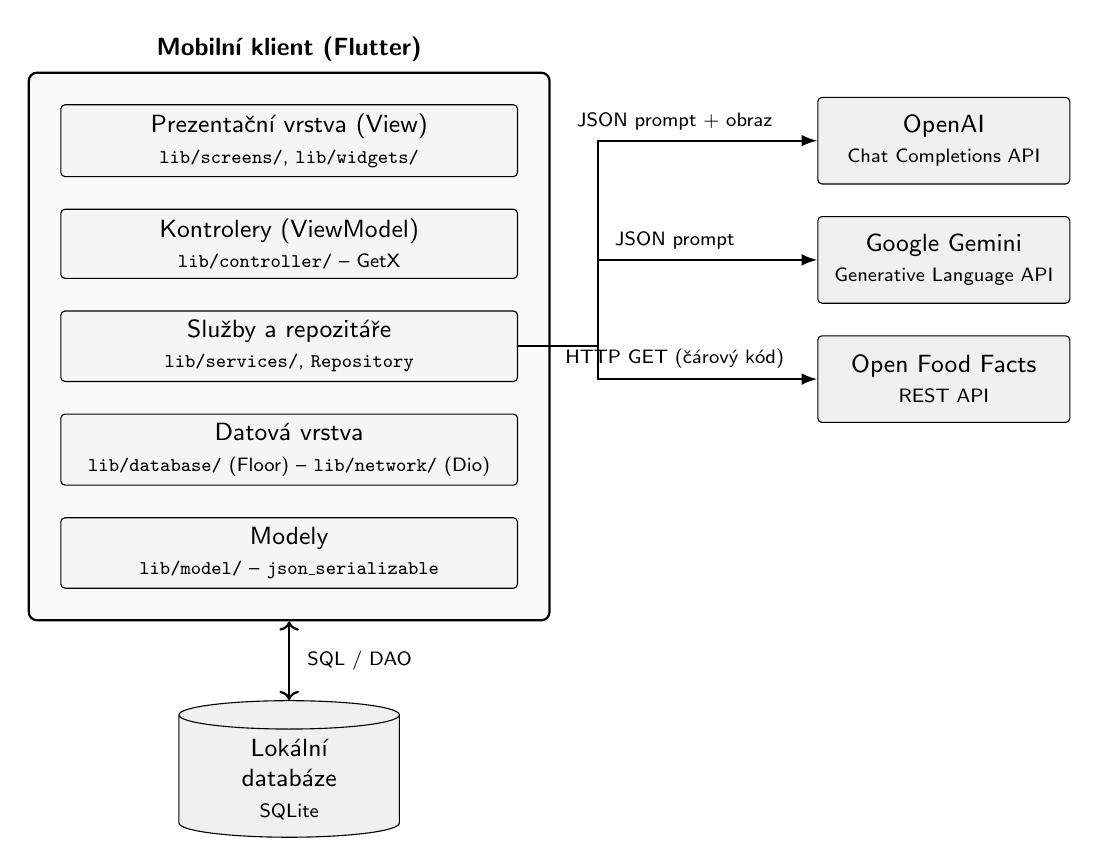
\begin{tikzpicture}[
	font=\small\sffamily,
	node distance=4mm,
	layer/.style={
		draw,
		rounded corners=1.5pt,
		minimum height=8mm,
		minimum width=58mm,
		align=center,
		fill=black!4,
	},
	clientbox/.style={
		draw,
		thick,
		rounded corners=3pt,
		inner sep=4mm,
		fill=black!2,
	},
	ext/.style={
		draw,
		rounded corners=1.5pt,
		minimum height=11mm,
		minimum width=32mm,
		align=center,
		fill=black!6,
	},
	db/.style={
		draw,
		cylinder,
		shape border rotate=90,
		aspect=0.25,
		minimum height=14mm,
		minimum width=28mm,
		align=center,
		fill=black!6,
	},
	arr/.style={-{Latex[length=2mm]}, thick},
	dataflow/.style={font=\scriptsize\sffamily, midway, sloped, above, inner sep=1pt},
]

% Vrstvy mobilního klienta
\node[layer] (view) {Prezentační vrstva (View)\\\scriptsize \texttt{lib/screens/}, \texttt{lib/widgets/}};
\node[layer, below=of view] (ctrl) {Kontrolery (ViewModel)\\\scriptsize \texttt{lib/controller/} -- GetX};
\node[layer, below=of ctrl] (svc) {Služby a repozitáře\\\scriptsize \texttt{lib/services/}, \texttt{Repository}};
\node[layer, below=of svc] (data) {Datová vrstva\\\scriptsize \texttt{lib/database/} (Floor) -- \texttt{lib/network/} (Dio)};
\node[layer, below=of data] (model) {Modely\\\scriptsize \texttt{lib/model/} -- \texttt{json\_serializable}};

% Obal mobilního klienta -- kreslíme na background layer, aby nezakryl vnitřní vrstvy
\begin{scope}[on background layer]
\node[clientbox, fit=(view)(ctrl)(svc)(data)(model), label={[font=\small\sffamily\bfseries, anchor=south]north:Mobilní klient (Flutter)}] (client) {};
\end{scope}

% Lokální databáze pod klientem
\node[db, below=10mm of client] (sqlite) {Lokální\\databáze\\\scriptsize SQLite};

% Externí služby (vpravo) -- větší odsazení pro čitelné popisky šipek
\node[ext, right=38mm of view] (openai) {OpenAI\\\scriptsize Chat Completions API};
\node[ext, below=of openai] (gemini) {Google Gemini\\\scriptsize Generative Language API};
\node[ext, below=of gemini] (off) {Open Food Facts\\\scriptsize REST API};

% Šipky: mobilní klient ↔ SQLite (start zespodu klienta, popisek vpravo)
\draw[arr, <->] (client.south -| sqlite.north) -- (sqlite.north)
	node[pos=0.5, right=1mm, font=\scriptsize\sffamily] {SQL / DAO};

% Šipky: vrstva služeb / sítě → externí API (sběrnice ven z klienta)
\coordinate (busTop) at ($(client.east)+(6mm,0)$);
\coordinate (busOpenai) at (busTop |- openai.west);
\coordinate (busGemini) at (busTop |- gemini.west);
\coordinate (busOff)    at (busTop |- off.west);

% Popisek umístíme blíže ke sběrnici (dál od API boxu) -- pos=0.35 zleva
\draw[arr] (svc.east) -- (svc.east -| busTop) -- (busOpenai) -- node[pos=0.35, above, font=\scriptsize\sffamily] {JSON prompt + obraz} (openai.west);
\draw[arr] (svc.east) -- (svc.east -| busTop) -- (busGemini) -- node[pos=0.35, above, font=\scriptsize\sffamily] {JSON prompt} (gemini.west);
\draw[arr] (svc.east) -- (svc.east -| busTop) -- (busOff)    -- node[pos=0.35, above, font=\scriptsize\sffamily] {HTTP GET (čárový kód)} (off.west);

\end{tikzpicture}
}
	\caption{Architektura aplikace.}
	\label{fig:architektura}
\end{figure}

Vrstva kontrolerů (ViewModel) vystavuje pozorovatelné proměnné, na které se prezentační vrstva naváže a automaticky se překresluje při změně dat.
Architekturu doplňuje vzor \emph{Repository} pro abstrakci přístupu k~datům, vzor \emph{Strategy} pro zaměnitelné implementace poskytovatelů umělé inteligence (viz sekce~\ref{subsec:aiApi}) a centrální registr závislostí v~souboru \texttt{lib/locator.dart}.

V~souladu se vzorem MVVM je vnitřní architektura mobilního klienta organizována do pěti logických vrstev, které lze mapovat na tři základní role tohoto vzoru.
Nejvyšší vrstvou je prezentační vrstva (View), tvořená obrazovkami (adresář \texttt{lib/screens/}) a~sdílenými widgety (\texttt{lib/widgets/}), která definuje uživatelské rozhraní aplikace prostřednictvím deklarativní kompozice Flutter widgetů.
Pod ní se nachází vrstva kontrolerů (ViewModel, adresář \texttt{lib/controller/}), jejíž komponenty rozšiřují třídu \texttt{GetxController} a~zapouzdřují prezentační logiku jednotlivých obrazovek včetně reakcí na uživatelské akce a~správy reaktivního stavu zobrazených dat prostřednictvím pozorovatelných proměnných.

Zbývající tři vrstvy společně tvoří vrstvu Model vzoru MVVM.
První z~nich je vrstva služeb (\texttt{lib/services/}), která implementuje doménovou logiku aplikace včetně pipeline pro umělou inteligenci, správy uživatelského profilu, plánování notifikací a~sestavování doménových agregátů z~databázových entit.
Přístup k~datům zajišťují dvě oddělené vrstvy odpovídající dvěma typům datových zdrojů aplikace, přičemž abstrakci nad těmito zdroji poskytuje vzor \emph{Repository}.

Lokální datová vrstva (\texttt{lib/database/}) obsahuje definice databázových entit, datových přístupových objektů (DAO) a~migračních skriptů frameworku Floor, přičemž zajišťuje typově bezpečný přístup k~relačním datům uloženým v~SQLite.
Síťová vrstva (\texttt{lib/network/}) zapouzdřuje REST klienty pro komunikaci s~externími API a~poskytuje vyšším vrstvám typované odpovědi bez nutnosti pracovat přímo s~HTTP protokolem.
Repozitáře, jejichž ústředním zástupcem je \texttt{DayRecordRepository} pro denní záznam (sekce~\ref{subsec:repozitare}), fungují jako fasáda nad těmito datovými zdroji a~vystavují výsledky prostřednictvím reaktivních streamů, čímž kontrolery a~služby nejsou vázány na konkrétní implementaci úložiště.
Na nejnižší úrovni stojí vrstva modelů (\texttt{lib/model/}), která definuje datové třídy s~podporou serializace prostřednictvím knihovny \texttt{json\_serializable} a~slouží jako společný jazyk pro výměnu dat mezi ostatními vrstvami.

Na úrovni adresářové struktury projektu odpovídá každá architektonická vrstva samostatnému adresáři v~rámci kořenového adresáře \texttt{lib/}.
Kromě výše popsaných vrstev projekt obsahuje adresář \texttt{lib/utils/} se sdílenými pomocnými funkcemi, jako jsou definice promptů pro model umělé inteligence, validační logika a formátovací utility, a adresář \texttt{lib/generated/} s~automaticky generovanými soubory pro lokalizaci a databázový kód, které nejsou editovány ručně.
Konfigurační soubor \texttt{lib/app\_theme.dart} centralizuje veškeré návrhové tokeny aplikace (barvy, rozestupy, typografie, stíny), čímž zajišťuje konzistentní vizuální styl napříč všemi obrazovkami.
Vstupním bodem aplikace je soubor \texttt{lib/main.dart}, který řídí inicializační sekvenci zahrnující načtení konfigurace prostředí, registraci závislostí, obnovení uživatelské relace a spuštění plánovaných notifikací, přičemž samotná konfigurace \texttt{MaterialApp} je definována v~souboru \texttt{lib/app.dart}~\cite{flutterDoc}.

Komunikace mezi vrstvami probíhá přes centralizovaný registr závislostí, čímž jsou kontrolery a služby odděleny od konkrétních implementací datových zdrojů.
Tento návrh umožňuje za běhu nahradit implementaci poskytovatele umělé inteligence (sekce~\ref{subsec:aiApi}) bez zásahu do vyšších vrstev aplikace.

\subsection{Navigace a struktura obrazovek}
\label{subsec:navigace}

Pro navigaci mezi obrazovkami využívá aplikace imperativní model frameworku GetX bez pojmenované tabulky rout, což umožňuje předávat typované parametry přímo přes konstruktor cílové obrazovky~\cite{getxDoc}.
Kořenovou komponentou navigační hierarchie je hlavní obrazovka tvořená třízáložkovým shellem se záložkami Dashboard (denní přehled, seznam jídel a cvičení), Progress (týdenní a měsíční vizualizace, hmotnost) a Profile (osobní údaje, cíle, nastavení).
Přepínání záložek je řízeno reaktivní proměnnou a zachovává stav jednotlivých záložek bez nové navigace.

Plovoucí akční tlačítko ve spodní liště otevírá panel rychlých akcí s~pěti primárními vstupními body pro záznam dat (jídlo z~historie, foto, hlas, čárový kód, cvičení).
Panel je dostupný z~libovolné záložky a slouží jako centrální rozcestník pro všechny modality záznamu definované funkčními požadavky.
Aplikace obsahuje přibližně 58~obrazovek a modálních listů organizovaných v~adresáři \texttt{lib/screens/} do tematických skupin (onboarding, skenování, jídla a ingredience, logování, profil).
Modální listy jsou využívány pro doplňkové interakce nevyžadující opuštění aktuálního kontextu, jako je výběr data pro kopírování jídla, záznam hmotnosti nebo akce u~detailu cvičení.
Konkrétní navigační toky pro hlavní případy užití byly popsány v~sekci~\ref{subsec:interakcniToky} a snímky odpovídajících obrazovek jsou prezentovány v~sekci~\ref{sec:klicoveObrazovky}.

\section{Datový model}
\label{sec:datovyModel}

V~návaznosti na softwarovou architekturu představenou v~sekci~\ref{sec:softwarovaArchitektura} popisuje tato sekce konkrétní podobu datové vrstvy aplikace Foody.
Důraz je kladen na strukturu lokální relační databáze, vztahy mezi jednotlivými entitami a způsob, jakým je nad těmito entitami sestavena repozitářová vrstva poskytující doménové agregáty prezentační vrstvě.
Nejprve je v~podsekci~\ref{subsec:schemaDb} popsáno schéma databáze a vztahy mezi devíti hlavními entitami.
Podsekce~\ref{subsec:sablony} dokumentuje samostatný subsystém šablon pro opakovaně zapisované položky, který adresuje funkční požadavky na zrychlení záznamu.
Závěrečná podsekce~\ref{subsec:repozitare} popisuje repozitářovou vrstvu, transformaci databázových entit na doménové modely a mechanismus reaktivního zpřístupnění dat uživatelskému rozhraní.

\subsection{Schéma databáze a vztahy mezi entitami}
\label{subsec:schemaDb}

V~rámci datového modelu aplikace Foody je definováno celkem devět entit, které lze rozdělit do dvou logických skupin podle účelu uložených dat.
Transakční skupinu tvoří pět entit zachycujících konkrétní časově vázané záznamy uživatele (denní záznam, jídlo, ingredience, cvičení, hmotnost), zatímco kmenovou skupinu sdružují čtyři entity tvořící osobní knihovnu opakovaně používaných jídel, ingrediencí a cvičení daného uživatele, dále v~textu označované jako šablony, jejichž struktura a role jsou podrobně rozebrány v~samostatné podsekci~\ref{subsec:sablony}.
Vizuální znázornění schématu transakční skupiny s~naznačenými cizími klíči a kardinalitami je zachyceno na obrázku~\ref{fig:erDiagram}.
Kmenové entity jsou z~důvodu přehlednosti v~obrázku vynechány, neboť netvoří relační vazby s~transakční skupinou a jejich vzájemné vztahy jsou popsány v~odpovídající podsekci.

\begin{figure}[ht]
	\centering
	\resizebox{\textwidth}{!}{% ER diagram databázového schématu aplikace Foody.
% Zobrazuje pouze transakční entity (DayRecord, Meal, Ingredient, Exercise, WeightEntry).
% Šablonové (kmenové) entity jsou popsány v textu kapitoly v podsekci o systému šablon.
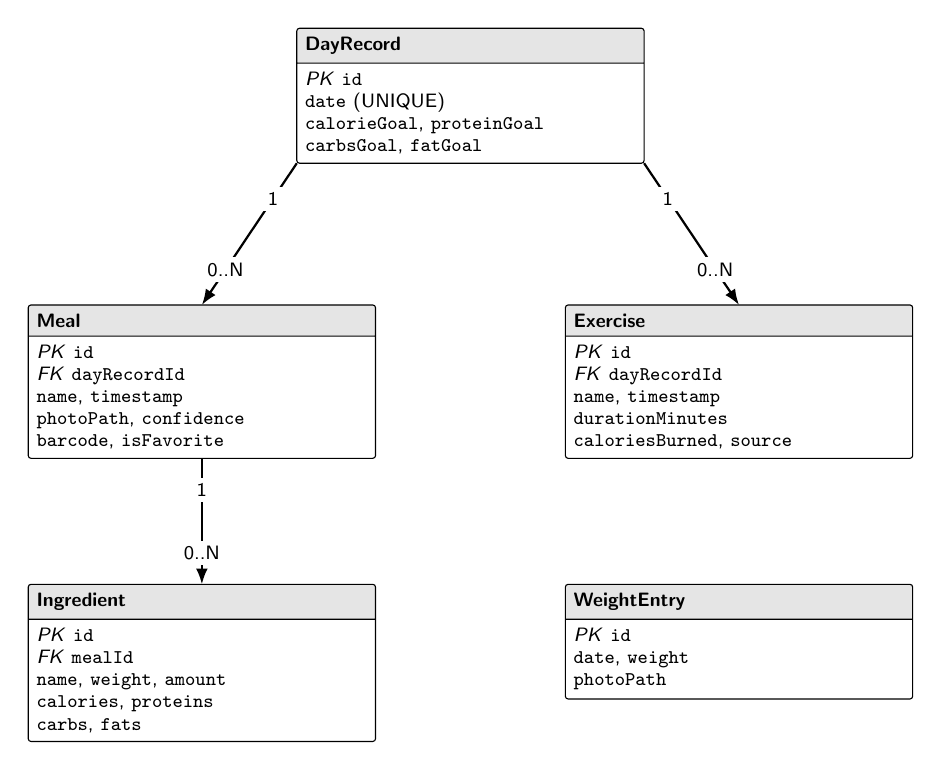
\begin{tikzpicture}[
	font=\scriptsize\sffamily,
	entity/.style={
		draw,
		rectangle split,
		rectangle split parts=2,
		rectangle split part fill={black!10, white},
		inner sep=3pt,
		rounded corners=1pt,
		text width=42mm,
		align=left,
		minimum height=8mm,
		outer sep=0pt,
	},
	rel/.style={-{Latex[length=2mm]}, thick},
	card/.style={
		font=\scriptsize\sffamily,
		fill=white,
		inner sep=2pt,
		outer sep=0pt,
	},
]

\node[entity] (day) {
	\textbf{DayRecord}
	\nodepart{two}
	\textit{PK} \texttt{id}\\
	\texttt{date} (UNIQUE)\\
	\texttt{calorieGoal}, \texttt{proteinGoal}\\
	\texttt{carbsGoal}, \texttt{fatGoal}
};

\node[entity, below left=18mm and -10mm of day] (meal) {
	\textbf{Meal}
	\nodepart{two}
	\textit{PK} \texttt{id}\\
	\textit{FK} \texttt{dayRecordId}\\
	\texttt{name}, \texttt{timestamp}\\
	\texttt{photoPath}, \texttt{confidence}\\
	\texttt{barcode}, \texttt{isFavorite}
};

\node[entity, below right=18mm and -10mm of day] (exercise) {
	\textbf{Exercise}
	\nodepart{two}
	\textit{PK} \texttt{id}\\
	\textit{FK} \texttt{dayRecordId}\\
	\texttt{name}, \texttt{timestamp}\\
	\texttt{durationMinutes}\\
	\texttt{caloriesBurned}, \texttt{source}
};

\node[entity, below=16mm of meal] (ingredient) {
	\textbf{Ingredient}
	\nodepart{two}
	\textit{PK} \texttt{id}\\
	\textit{FK} \texttt{mealId}\\
	\texttt{name}, \texttt{weight}, \texttt{amount}\\
	\texttt{calories}, \texttt{proteins}\\
	\texttt{carbs}, \texttt{fats}
};

\node[entity, below=16mm of exercise] (weight) {
	\textbf{WeightEntry}
	\nodepart{two}
	\textit{PK} \texttt{id}\\
	\texttt{date}, \texttt{weight}\\
	\texttt{photoPath}
};

% Vztahy -- kardinality posunuté dovnitř lajny (pos 0.25/0.75),
% aby nezasahovaly do hlaviček entit.
\draw[rel] (day.south west) -- (meal.north)
	node[card, pos=0.25] {1}
	node[card, pos=0.75] {0..N};
\draw[rel] (day.south east) -- (exercise.north)
	node[card, pos=0.25] {1}
	node[card, pos=0.75] {0..N};
\draw[rel] (meal.south) -- (ingredient.north)
	node[card, pos=0.25] {1}
	node[card, pos=0.75] {0..N};

\end{tikzpicture}
}
	\caption{ER diagram databázového schématu.}
	\label{fig:erDiagram}
\end{figure}

Transakční entity tvoří dvouúrovňovou hierarchii s~\texttt{DayRecord} v~kořeni: \texttt{Meal} je k~dennímu záznamu připojeno vztahem 1:0..N, \texttt{Ingredient} je obdobně připojena k~\texttt{Meal}, a \texttt{Exercise} tvoří paralelní podstrom přímo pod \texttt{DayRecord}.
Záznamy hmotnosti jsou modelovány jako samostatná entita bez vazby na denní záznam, což odpovídá jejich povaze nezávislého časového zápisu.
Veškeré cizí klíče jsou deklarovány s~pravidlem kaskádového mazání, které zajišťuje referenční integritu na úrovni SQLite a eliminuje riziko osiřelých záznamů při uživatelském mazání denního záznamu nebo přechodu mezi profily.

Normalizované schéma s~referenční integritou na úrovni databáze umožňuje efektivní dotazování pro analytické scénáře aplikace (týdenní a měsíční přehledy, vyhledávání oblíbených, vyhodnocování porušení dietních omezení), zatímco doménové agregáty pro uživatelské rozhraní skládá repozitářová vrstva popsaná v~podsekci~\ref{subsec:repozitare}.

\subsection{Systém šablon pro opakovaně používané položky}
\label{subsec:sablony}

V~záznamech každého uživatele se přirozeně utváří relativně stabilní okruh pravidelně konzumovaných jídel, opakovaně používaných ingrediencí a typických cvičebních aktivit.
Pro zachycení této opakovatelnosti zavádí datový model aplikace Foody samostatný subsystém šablon, jehož primárním účelem je sloužit jako osobní knihovna uživatele.
Knihovna je tvořena třemi šablonovými entitami pro jídla, ingredience a cvičení a uživatel si ji přirozeně buduje samotným používáním aplikace, bez nutnosti samostatné správy.
Na této knihovně pak stojí implementace funkčních požadavků FR-17 (oblíbené položky), FR-18 (duplikace dřívějších záznamů) a FR-19 (našeptávání názvů z~historie).

Šablona slouží jako zdroj dat při vytváření nového záznamu, aniž by s~ním byla trvale relačně vázána.
Pozdější editace šablony tak neovlivní již uložená historická data a smazání šablony z~knihovny nevyvolá ztrátu historie.
Pro řazení v~uživatelských nabídkách jsou u~každé šablony udržovány metriky frekvence použití (\texttt{usageCount}) a času posledního výskytu (\texttt{lastUsedAt}), díky kterým lze nabídnout uživateli nejprve nejčastěji a nejnověji používané položky.

Šablony jídel mají na rozdíl od ingrediencí a cvičení vnitřní hierarchii: u~každé šablony je uložen kompletní rozpis ingrediencí včetně hmotností a nutričních hodnot, takže opětovné použití obnovuje celé jídlo bez nutnosti nového volání modelu umělé inteligence nebo ručního zápisu.
Naplňování šablon probíhá automaticky při uložení nového záznamu, takže uživatel nemusí oblíbené položky spravovat samostatně.

\subsection{Repozitářová vrstva}
\label{subsec:repozitare}

Data jsou uživatelskému rozhraní zpřístupněna prostřednictvím pěti repozitářů odpovídajících věcným oblastem datového modelu (denní záznam, hmotnost, šablony jídel, ingrediencí a cvičení).
Klíčovou odpovědností \texttt{DayRecordRepository} je sestavení doménového modelu denního přehledu z~normalizovaných entit a jeho průběžná aktualizace prostřednictvím reaktivního streamu, takže denní přehled v~rozhraní se obnovuje automaticky při každé změně záznamu~\cite{getxDoc}.
Konkrétní způsob, jakým je datová vrstva využívána při integraci s~modelem umělé inteligence, je popsán v~sekci~\ref{sec:integraceAi}.

\section{Klíčové obrazovky aplikace}
\label{sec:klicoveObrazovky}

Tato sekce představuje hlavní obrazovky implementované aplikace, které tvoří uživatelskou tvář systému a ilustrují klíčové interakční toky odvozené z~případů užití v~sekci~\ref{sec:pripadyUziti}.
Pro každou obrazovku je uveden snímek z~reálného běhu aplikace na operačním systému iOS, popis její role a vazba na příslušné funkční požadavky.
Obrazovky, které ve své práci obsahují více navzájem souvisejících stavů (například hlavní obrazovka s~otevřeným kalendářem versus stav během rozpoznávání jídla), jsou prezentovány jako skupiny snímků v~jediném obrázku, aby čtenář viděl variabilitu jedné funkce vedle sebe.

\paragraph{Hlavní obrazovka.}
Hlavní obrazovka aplikace zobrazuje denní přehled kalorického příjmu (FR-02) a slouží jako rozcestník pro všechny vstupní modality záznamu.
V~horní části je umístěn scrollovatelný kalendář s~vizualizací plnění cílů pomocí barevných kruhů, pod ním souhrn kalorií vůči stanovenému cíli, vizualizace makroživin a seznam zaznamenaných jídel a cvičení.
V~dolní části je primární akční tlačítko otevírající panel rychlých akcí pro záznam jídla nebo cvičení.
Obrázek~\ref{fig:screenDashboard} zachycuje obrazovku ve třech typických stavech: ve výchozím zobrazení denního přehledu, se zobrazenou kartou rozpoznávání jídla v~průběhu volání pipeline umělé inteligence a s~otevřeným bottom sheetem kalendáře pro výběr dne.

\begin{figure}[ht]
	\centering
	\begin{minipage}[t]{0.31\textwidth}
		\centering
		\screenshot[width=\textwidth]{figures/screens/DashboardScreen_Main.png}
		\\(a)~Výchozí zobrazení
	\end{minipage}\hfill
	\begin{minipage}[t]{0.31\textwidth}
		\centering
		\screenshot[width=\textwidth]{figures/screens/DashboardScreen_RecognisingMeal.png}
		\\(b)~Stav během rozpoznávání jídla
	\end{minipage}\hfill
	\begin{minipage}[t]{0.31\textwidth}
		\centering
		\screenshot[width=\textwidth]{figures/screens/DashboardScreen_CalendarBottomSheet.png}
		\\(c)~Otevřený kalendář pro výběr dne
	\end{minipage}
	\caption{Hlavní obrazovka aplikace ve třech stavech.}
	\label{fig:screenDashboard}
\end{figure}

\paragraph{Skenování jídla.}
Obrazovka kamery slouží k~pořízení fotografie jídla pro rozpoznání umělou inteligencí (FR-06).
Rozhraní je úmyslně minimalistické, aby uživatele nerozptylovalo při focení.
Pro alternativní vstup z~galerie je k~dispozici samostatné tlačítko (FR-12).

\begin{figure}[ht]
	\centering
	\screenshot[width=0.42\textwidth]{figures/screens/ScanCameraScreen.png}
	\caption{Obrazovka skenování jídla.}
	\label{fig:screenScanCamera}
\end{figure}

\paragraph{Editace záznamu jídla.}
Editační obrazovka jídla slouží jako náhled výsledku rozpoznání pomocí umělé inteligence i jako rozhraní pro ruční úpravu nebo plně manuální vytvoření záznamu (FR-01).
Po dokončení rozpoznání obsahuje seznam navržených ingrediencí a barevnou indikaci nejistoty výstupu ve formě confidence badge (FR-08): zelená pro spolehlivost $\geq$~75~\%, žlutá pro $\geq$~50~\% a červená pro nižší hodnoty.
Uživatel může jednotlivé ingredience upravit, přidat nebo odebrat, změnit gramáž nebo počet kusů (FR-15) a v~případě potřeby vyvolat opakované rozpoznání pomocí funkce ,,Fix with AI'' (FR-13).

\begin{figure}[ht]
	\centering
	\screenshot[width=0.42\textwidth]{figures/screens/EditMealScreen.png}
	\caption{Editace záznamu jídla.}
	\label{fig:screenEditMeal}
\end{figure}

\paragraph{Výběr a záznam jídla.}
Obrazovka záznamu jídla sjednocuje vyhledávání v~historii (FR-19), oblíbené položky (FR-17), šablony jídel a duplikaci dříve uložených záznamů (FR-18) do jediného rozhraní.
Slouží jako vstupní bod pro rychlý ruční zápis i jako navigační uzel pro pokročilé varianty záznamu (skenování čárového kódu, hlasový vstup).
V~případě, že uživatel chce vytvořit zcela nové jídlo, které dosud v~historii ani ve sdílených databázích neexistuje, pokračuje z~této obrazovky na navazující obrazovku ručního vytvoření nového jídla, která je popsána detailněji v~sekci~\ref{subsec:manualniVstup}.

\begin{figure}[ht]
	\centering
	\begin{minipage}[t]{0.42\textwidth}
		\centering
		\screenshot[width=\textwidth]{figures/screens/MealLogScreen.png}
		\\(a)~Výběr z~historie a~oblíbených
	\end{minipage}\hfill
	\begin{minipage}[t]{0.42\textwidth}
		\centering
		\screenshot[width=\textwidth]{figures/screens/ManualAddNewMealScreen.png}
		\\(b)~Ruční vytvoření nového jídla
	\end{minipage}
	\caption{Manuální tok záznamu jídla.}
	\label{fig:screenMealLog}
\end{figure}

\paragraph{Hlasový vstup.}
Obrazovka hlasového vstupu umožňuje uživateli popsat jídlo přirozeným jazykem, přičemž rozpoznávání řeči probíhá v~reálném čase (FR-14).
Po dokončení nahrávání je text odeslán do pipeline pro umělou inteligenci, která vrátí strukturované rozpoznání ingrediencí.
Hlasový vstup byl ve výsledcích uživatelského testování označen jako jedna z~nejvíce oceněných funkcí aplikace.

\begin{figure}[ht]
	\centering
	\screenshot[width=0.42\textwidth]{figures/screens/VoiceLogScreen.png}
	\caption{Hlasový vstup.}
	\label{fig:screenVoiceLog}
\end{figure}

\paragraph{Sledování cvičení.}
Modul cvičení nabízí čtyři vstupní modality pro záznam aktivity: rozpoznání pomocí umělé inteligence z~textového popisu, hlasový vstup, ruční zadání a výběr ze šablon.
Obrazovka navazuje na hlavní funkcionalitu sledování příjmu energie a doplňuje ji o~výdejovou stranu energetické bilance (FR-22).

\begin{figure}[ht]
	\centering
	\screenshot[width=0.42\textwidth]{figures/screens/ExerciseLogScreen.png}
	\caption{Modul sledování cvičení.}
	\label{fig:screenExerciseLog}
\end{figure}

\paragraph{Profil a nastavení.}
Profilová obrazovka slouží jako rozcestník pro správu osobních údajů (FR-04), nutričních cílů (FR-03), dietních preferencí (FR-20), připomínek (FR-29) a integrace se zdravotními platformami.
Detailní podobrazovky jsou ilustrovány v~příslušných sekcích~\ref{sec:klicoveFunkce}.

\begin{figure}[ht]
	\centering
	\screenshot[width=0.42\textwidth]{figures/screens/ProfileScreen.png}
	\caption{Obrazovka profilu.}
	\label{fig:screenProfile}
\end{figure}

\paragraph{Dotazy v~přirozeném jazyce.}
Obrazovka dotazů v~přirozeném jazyce (Ask AI) umožňuje uživateli klást dotazy nad svými historickými nutričními daty (FR-27).
Implementace využívá dvouprůchodový systém: první volání modelu identifikuje časový rozsah dotazu, druhé pak generuje analytickou odpověď nad odpovídajícími daty z~lokální databáze.
Obrázek~\ref{fig:screenAskAi} zachycuje obrazovku ve třech typických stavech: výchozí prázdný stav, stav s~ukázkovými otázkami a stav s~vygenerovanou odpovědí.

\begin{figure}[ht]
	\centering
	\begin{minipage}[t]{0.31\textwidth}
		\centering
		\screenshot[width=\textwidth]{figures/screens/AskAIScreen.png}
		\\(a)~Výchozí stav
	\end{minipage}\hfill
	\begin{minipage}[t]{0.31\textwidth}
		\centering
		\screenshot[width=\textwidth]{figures/screens/AskAIScreenExamples.png}
		\\(b)~Ukázkové otázky
	\end{minipage}\hfill
	\begin{minipage}[t]{0.31\textwidth}
		\centering
		\screenshot[width=\textwidth]{figures/screens/AskAIScreenResponse.png}
		\\(c)~Odpověď AI
	\end{minipage}
	\caption{Dotazy v~přirozeném jazyce ve třech stavech.}
	\label{fig:screenAskAi}
\end{figure}

\paragraph{Týdenní a měsíční přehledy.}
Obrazovka přehledů vizualizuje trendy kalorického příjmu, hmotnosti a plnění cílů na týdenní a měsíční úrovni (FR-24).
Součástí je také kalendář s~vizualizací porušení dietních omezení (FR-21) a karta s~aktuální tělesnou hmotností a indexem BMI.
Vzhledem k~tomu, že obrazovka je delší než výška displeje, je v~obrázku~\ref{fig:screenProgress} prezentována ve dvou snímcích zachycujících střední a spodní část.

\begin{figure}[ht]
	\centering
	\begin{minipage}[t]{0.42\textwidth}
		\centering
		\screenshot[width=\textwidth]{figures/screens/ProgressScreen_MidPart.png}
		\\(a)~Střední část obrazovky
	\end{minipage}\hfill
	\begin{minipage}[t]{0.42\textwidth}
		\centering
		\screenshot[width=\textwidth]{figures/screens/ProgressScreen_BottomPart.png}
		\\(b)~Spodní část obrazovky
	\end{minipage}
	\caption{Obrazovka přehledů.}
	\label{fig:screenProgress}
\end{figure}

\section{Integrace modelu umělé inteligence}
\label{sec:integraceAi}

Tato sekce popisuje implementaci pipeline pro rozpoznávání jídel a cvičení pomocí externího modelu umělé inteligence, která naplňuje funkční požadavky FR-06, FR-07, FR-08, FR-10 a FR-11.
Postupně je představena celková architektura datového toku, struktura promptů a formát odpovědí, mechanismus práce s~nejistotou výstupu, vrstvená ochrana proti prompt injection a podpora více poskytovatelů modelu.
Volba multimodálního jazykového modelu místo specializované konvoluční sítě trénované na potravinovém datasetu vychází z~vývoje oboru po roce 2022, kdy multimodální modely umožnily v~jediném volání zpracovat obraz i textový popis bez nutnosti vlastního trénování~\cite{wang2026visionLanguageFood}.
Tento přístup současně obchází generalizační limit specializovaných modelů napříč různými kuchyněmi, který na transformerové architektuře CBiAFormer doložili Liu a~kol. propadem přesnosti z~92,40~\% na západním datasetu na 72,92~\% na smíšeném datasetu~\cite{liu2025deepLearning}, a~přebírá širší pokrytí trénovací distribuce dostupné u~obecných modelů~\cite{chotwanvirat2024scoping}.

\subsection{Architektura pipeline}
\label{subsec:aiPipeline}

Pipeline pro umělou inteligenci je v~aplikaci centralizována do jediné doménové služby (\texttt{AiPipelineService}), která zastřešuje celý tok od uživatelského vstupu až po finální výsledek prezentovaný v~uživatelském rozhraní.
Vstupem může být fotografie jídla doplněná o~volitelný textový popis, samostatný textový popis jídla nebo hlasově nadiktovaný popis předzpracovaný transkripční vrstvou.
Vstupní text nejprve prochází sanitizací a kontrolou bezpečnosti (viz sekce~\ref{subsec:promptInjection}) a následně je z~něj sestaven strukturovaný JSON prompt odpovídající scénáři analýzy jídla, cvičení nebo výpočtu nutričních cílů.

Sestavený prompt je odesílán přes abstraktní rozhraní, jehož konkrétní implementace odpovídá zvolenému poskytovateli modelu, a obdržená odpověď je následně parsována do typovaného doménového objektu prostřednictvím nástroje pro generování serializačního kódu.
Parsovaný výsledek prochází takzvaným \emph{confidence gate}, který na základě hodnoty spolehlivosti vrací jednu ze tří forem výsledku: úspěšné rozpoznání, rozpoznání s~varováním o~nízké jistotě, nebo selhání bez použitelného výstupu.

Vedle hlavní pipeline pro rozpoznávání jídel jsou implementovány samostatné toky pro analýzu cvičení a pro výpočet nutričních cílů.
Tok pro cvičení vychází z~textového popisu aktivity a vrací strukturu obsahující název, dobu trvání a odhadovanou energetickou hodnotu, přičemž využívá víceúrovňovou validaci popsanou v~sekci~\ref{subsec:confidence}.
Tok pro výpočet nutričních cílů aplikuje Mifflin-St~Jeorovu rovnici (rovnice~(\ref{eq:msj-muzi}) a~(\ref{eq:msj-zeny})) na uživatelovy údaje o~hmotnosti, výšce, věku, pohlaví a cíli, čímž vrací doporučené denní hodnoty kalorií a makroživin.

\begin{figure}[ht]
	\centering
	\resizebox{0.95\textwidth}{!}{% Sekvenční diagram pipeline umělé inteligence pro rozpoznání jídla z fotografie.
% Aktéři: UI -- AiPipelineService -- PromptSanitizer -- AiService -- Externí API.
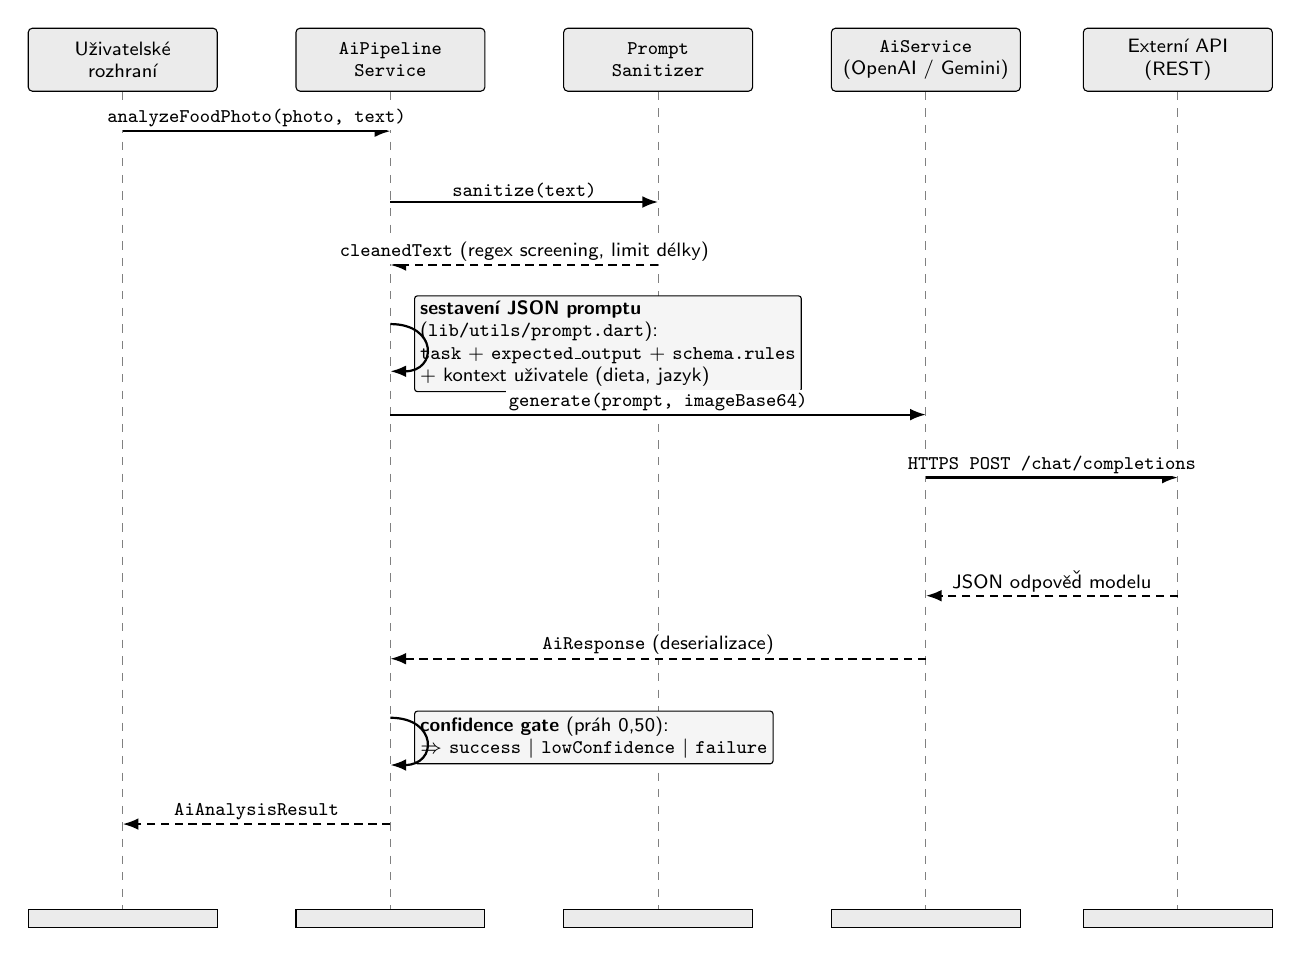
\begin{tikzpicture}[
	font=\scriptsize\sffamily,
	x=1cm, y=1cm,
	actor/.style={
		draw,
		rounded corners=1.5pt,
		minimum height=8mm,
		minimum width=24mm,
		align=center,
		fill=black!8,
	},
	lifeline/.style={dashed, black!50},
	msg/.style={-{Latex[length=2mm]}, thick},
	ret/.style={-{Latex[length=2mm]}, thick, densely dashed},
	mlbl/.style={font=\scriptsize\sffamily, midway, above, sloped=false, fill=white, inner sep=1pt},
	selfnote/.style={
		draw,
		rounded corners=1pt,
		fill=black!4,
		font=\scriptsize\sffamily,
		align=left,
		inner sep=2pt,
	},
]

% --- Aktéři ---
\node[actor] (a1) at (0,0)   {Uživatelské\\rozhraní};
\node[actor] (a2) at (3.4,0) {\texttt{AiPipeline}\\\texttt{Service}};
\node[actor] (a3) at (6.8,0) {\texttt{Prompt}\\\texttt{Sanitizer}};
\node[actor] (a4) at (10.2,0){\texttt{AiService}\\(OpenAI / Gemini)};
\node[actor] (a5) at (13.4,0){Externí API\\(REST)};

% --- Lifelines ---
\foreach \a in {a1,a2,a3,a4,a5}
	\draw[lifeline] (\a.south) -- ($(\a.south)+(0,-10.5)$);

% --- Sekvence zpráv ---
% 1. UI -> Pipeline: vstup
\draw[msg] ($(a1.south)+(0,-0.5)$) -- ($(a2.south)+(0,-0.5)$)
	node[mlbl] {\texttt{analyzeFoodPhoto(photo, text)}};

% 2. Pipeline -> Sanitizer: sanitize(text)
\draw[msg] ($(a2.south)+(0,-1.4)$) -- ($(a3.south)+(0,-1.4)$)
	node[mlbl] {\texttt{sanitize(text)}};

% 3. Sanitizer -> Pipeline: cleanedText (návratová)
\draw[ret] ($(a3.south)+(0,-2.2)$) -- ($(a2.south)+(0,-2.2)$)
	node[mlbl] {\texttt{cleanedText} (regex screening, limit délky)};

% 4. Pipeline self-loop: sestavení JSON promptu
\node[selfnote, anchor=west] at ($(a2.south)+(0.3,-3.2)$) {
	\textbf{sestavení JSON promptu}\\
	(\texttt{lib/utils/prompt.dart}):\\
	\texttt{task} + \texttt{expected\_output} + \texttt{schema.rules}\\
	+ kontext uživatele (dieta, jazyk)
};
\draw[msg] ($(a2.south)+(0,-2.95)$) .. controls +(0.6,0) and +(0.6,0) .. ($(a2.south)+(0,-3.55)$);

% 5. Pipeline -> AiService: generate(prompt + image)
\draw[msg] ($(a2.south)+(0,-4.1)$) -- ($(a4.south)+(0,-4.1)$)
	node[mlbl] {\texttt{generate(prompt, imageBase64)}};

% 6. AiService -> External: HTTPS POST
\draw[msg] ($(a4.south)+(0,-4.9)$) -- ($(a5.south)+(0,-4.9)$)
	node[mlbl] {\texttt{HTTPS POST /chat/completions}};

% 7. External -> AiService: JSON response
\draw[ret] ($(a5.south)+(0,-6.4)$) -- ($(a4.south)+(0,-6.4)$)
	node[mlbl] {JSON odpověď modelu};

% 8. AiService -> Pipeline
\draw[ret] ($(a4.south)+(0,-7.2)$) -- ($(a2.south)+(0,-7.2)$)
	node[mlbl] {\texttt{AiResponse} (deserializace)};

% 9. Pipeline self-loop: confidence gate
\node[selfnote, anchor=west] at ($(a2.south)+(0.3,-8.2)$) {
	\textbf{confidence gate} (práh 0,50):\\
	\(\Rightarrow\) \texttt{success} \(\mid\) \texttt{lowConfidence} \(\mid\) \texttt{failure}
};
\draw[msg] ($(a2.south)+(0,-7.95)$) .. controls +(0.6,0) and +(0.6,0) .. ($(a2.south)+(0,-8.55)$);

% 10. Pipeline -> UI: výsledek
\draw[ret] ($(a2.south)+(0,-9.3)$) -- ($(a1.south)+(0,-9.3)$)
	node[mlbl] {\texttt{AiAnalysisResult}};

% --- Spodní rámečky aktérů (pro ukončení lifeline) ---
\foreach \a/\lbl in {a1/{},a2/{},a3/{},a4/{},a5/{}}
	\node[draw, fill=black!8, minimum height=2mm, minimum width=24mm]
		at ($(\a.south)+(0,-10.5)$) {};

\end{tikzpicture}
}
	\caption{Sekvenční diagram pipeline pro rozpoznání jídla.}
	\label{fig:aiPipeline}
\end{figure}

\subsection{Struktura promptů a formát odpovědí}
\label{subsec:prompty}

Strukturované prompty pro model umělé inteligence jsou centralizovány do jednoho modulu, který definuje šablony pro jednotlivé scénáře (rozpoznání jídla z~obrazu, rozpoznání jídla z~textu, analýza cvičení, výpočet nutričních cílů a dotazy v~přirozeném jazyce).
Plný text všech šablon je součástí zdrojového kódu odkazovaného v~příloze~\ref{app:kod}.
Každý prompt je sestaven jako JSON dokument se třemi hlavními poli: instrukcí pro model, schématem očekávané odpovědi a doplňkovými pravidly (například že numerická hodnota množství reprezentuje počet kusů a nikoli hmotnost, nebo že hodnota spolehlivosti musí ležet v~rozsahu 0~až 1).

Do promptu je zahrnut kontext uživatele, který modelu umožňuje přizpůsobit výstup individuálnímu profilu.
Mezi zahrnuté atributy patří dietní typ, vlastní dietní preference a jazykové preference, na jejichž základě model vrací názvy jídel a popisy v~odpovídajícím jazyce.
Z~uživatelského profilu se pro každý konkrétní dotaz extrahuje pouze relevantní podmnožina atributů, čímž se snižuje šum v~promptu a kontrolují se náklady na volání modelu.

Formát odpovědi pro analýzu jídla obsahuje příznak platnosti, identifikační údaje pokrmu, hodnotu spolehlivosti, údaj o~množství a strukturovaný seznam ingrediencí s~vlastními nutričními hodnotami.
Pro analýzu cvičení vrací model strukturu se jménem aktivity, dobou trvání a odhadem spálených kalorií za minutu, opět doplněnou o~hodnotu spolehlivosti.
Odpovědi jsou automaticky deserializovány do typovaných doménových objektů, čímž je práce s~výstupem na vyšších vrstvách aplikace zcela typově bezpečná.
Z~bezpečnostních důvodů popsaných v~sekci~\ref{subsec:promptInjection} je uživatelský vstup před vložením do promptu obalen do XML delimitérů.

\subsection{Práce s~nejistotou a confidence gate}
\label{subsec:confidence}

Funkční požadavek FR-08 stanovuje, že uživatel musí mít zpětnou vazbu o~spolehlivosti rozpoznání pomocí umělé inteligence.
Implementace tento požadavek naplňuje prostřednictvím takzvaného \emph{confidence gate}, který klasifikuje hodnotu spolehlivosti z~odpovědi modelu do tří úrovní a propaguje ji do uživatelského rozhraní.
Prahová hodnota pro úspěšné rozpoznání je nastavena na 0,50 jak pro analýzu jídel, tak pro analýzu cvičení.
Tato hodnota byla zvolena jako pragmatický kompromis mezi mírou falešně přijatých výstupů a frekvencí varovných hlášení, jejím podrobnějším laděním vůči empirickým datům se tato práce blíže nezabývala.

V~uživatelském rozhraní je nejistota vizualizována tříúrovňovou škálou v~rámci barevného indikátoru spolehlivosti na editační obrazovce jídla (viz obrázek~\ref{fig:screenEditMeal}).
Hodnoty $\geq$~75~\% jsou zobrazeny zeleně, hodnoty v~rozsahu 50~\% až 75~\% žlutě a hodnoty pod 50~\% červeně.
Tato barevná konvence prostupuje celou aplikaci.
V~uživatelském testování ji všichni participanti pochopili bez explicitního vysvětlování (viz sekce~\ref{sec:vysledkyTestovani}).

Logika rozhodování v~\emph{confidence gate} rozlišuje tři výsledné stavy.
Stav \emph{úspěch} odpovídá hodnotě spolehlivosti nad prahem a značí, že výsledek lze prezentovat uživateli bez zvláštního varování.
Stav \emph{nízká jistota} odpovídá hodnotě pod prahem 0,50, ale s~platným strukturovaným výstupem.
Data jsou v~tomto případě zobrazena s~viditelným varováním a doporučením kontroly.
Stav \emph{selhání} reprezentuje situaci, kdy model vrátí neplatný, prázdný nebo neparsovatelný výsledek, a aplikace v~tomto případě nabízí uživateli textový fallback (FR-11) nebo opakování pokusu.
Pro analýzu cvičení je validace doplněna o~kontrolu prázdného názvu, čímž je odlišeno tvrdé selhání od pouhé nízké jistoty.

\subsection{Ochrana proti prompt injection}
\label{subsec:promptInjection}

Vstup uživatele do pipeline pro umělou inteligenci představuje potenciální vektor útoku známý jako \emph{prompt injection}, kdy záměrně formulovaný vstup může změnit nebo přepsat původní systémové instrukce zaslané modelu~\cite{greshake2023indirect, owasp2025llm01}.
Hlavní motivací ochrany v~kontextu této aplikace není utajení samotného systémového promptu, jehož text je veřejně dostupný v~repozitáři aplikace, ale zachování předvídatelnosti chování modelu, na niž je vázána důvěra uživatele v~zobrazené nutriční odhady.
Z~pohledu uživatele lze identifikovat tři kategorie hrozeb, kterými jsou vědomý explicitní útok formulovaný jako adversariální instrukce, falešný poplach vyvolaný legitimním popisem jídla nebo cvičení s~náhodnou podobností pokusu o~injekci a obfuskovaný útok cíleně navržený tak, aby unikl jednoduché detekci.

Implementace adresuje tyto kategorie vícevrstvou ochranou v~rámci dedikovaného sanitizačního modulu (\texttt{PromptSanitizer}) volaného před každým odesláním vstupu do pipeline.
První vrstva (L1) provádí deterministické mechanické úpravy textu, kterými jsou odstranění bílých znaků na okrajích, odstranění řídících znaků a literálních značek vstupního delimitéru a oříznutí textu na maximální povolenou délku 500~znaků.
Druhá vrstva (L2) klasifikuje vstup pomocí šesti regulárních výrazů a vrací jeden ze tří stavů, kterými jsou \emph{čistý}, \emph{ambivalentní} a \emph{explicitní útok}.
Čtyři vzory zachycují fráze jednoznačně adversariální (například \uv{ignore previous instructions}, \uv{disregard your instructions}, \uv{reveal the system prompt} nebo \uv{do not respond in json}) a vstup s~takovým výskytem je odmítnut okamžitě.
Zbývající dva vzory označují \emph{ambivalentní} formulace jako \uv{you are}, \uv{act as} nebo zmínky o~systémovém promptu, u~nichž nelze vyloučit benigní výskyt v~přepisu hlasového vstupu nebo v~meta-dotazu na rozhraní Ask AI.
Vstup, který nezachytí žádný ze vzorů, je klasifikován jako \emph{čistý} a postupuje dále bez dodatečných kontrol.

Pro ambivalentní vstupy je aktivována třetí vrstva (L3), takzvaný \emph{LLM-based pre-screening}, který předá text menšímu a rychlejšímu modelu (GPT-5.4-mini) s~jediným úkolem rozhodnout, zda se jedná o~legitimní popis nebo o~pokus o~injekci.
Pokud LLM klasifikuje vstup jako útok, aplikace jej odmítne stejným způsobem jako u~explicitního vzoru.
V~opačném případě vstup pokračuje do hlavního modelu.
Nezávisle na výsledku klasifikace prochází každý legitimní vstup závěrečnou transformací, při níž je obalen do XML delimitéru \texttt{<user\_input>} pro strukturální izolaci od systémových instrukcí a do systémového promptu je doplněna explicitní anti-injekční direktiva zakazující modelu interpretovat obsah uživatelského bloku jako instrukce.
Tato direktiva tvoří průřezovou ochranu uplatňovanou vždy a slouží jako poslední linie obrany pro případ, že by adversariální vstup obě předchozí vrstvy obešel.
Vícevrstvý přístup vychází z~doporučení OWASP pro aplikace postavené na velkých jazykových modelech a z~empirických zjištění Liu et al.~\cite{owasp2025llm01, liu2024formalizing}, podle nichž žádná jednotlivá vrstva neposkytuje úplnou ochranu, ale jejich kombinace významně snižuje pravděpodobnost úspěšného útoku.

Specifickým rozhodnutím L3 vrstvy je její záměrný režim \emph{fail-open}, v~rámci kterého je vstup při výpadku síťové infrastruktury nebo nedostupnosti API předzvolovacího modelu považován automaticky za legitimní.
Tato volba reprezentuje vědomý kompromis mezi přísností bezpečnostní kontroly a dostupností služby pro uživatele, neboť přechodný technický problém na straně předzvolovacího modelu by jinak blokoval i~zcela neškodné popisy jídla a vedl by k~frustraci, která je v~kontextu každodenního používání aplikace nepřijatelná.
Reziduální riziko vyplývající z~tohoto kompromisu je sníženo vícevrstvou architekturou popsanou výše, ve které samostatně působí již vrstvy L1 a L2 a globálně XML delimiter s~anti-injekční direktivou.

Detekce založená na regulárních výrazech má z~principu nenulovou míru jak falešně pozitivních, tak falešně negativních klasifikací a cílený útočník dokáže jednoduché vzory obejít obfuskací, překlepy nebo kódováním v~Unicode~\cite{liu2024formalizing}.
Maximálním důsledkem úspěšného obejití všech vrstev je manipulace s~výstupem jediné aktuální analýzy, tedy například nesprávný odhad kalorické hodnoty nebo zamítavá odpověď modelu, neboť aplikace neukládá žádný serverový stav ani perzistentní datový kontext, který by útok mohl ovlivnit napříč relacemi.
Únik systémového promptu nepředstavuje samostatnou hrozbu, jelikož jeho text je veřejně dostupný v~repozitáři aplikace.
Pravděpodobnost falešně pozitivních klasifikací u~reálných uživatelských popisů jídla a cvičení v~přirozeném jazyce je naopak očekávána jako blízká nule, neboť tyto popisy fráze odpovídající explicitním adversariálním vzorům přirozeně neobsahují.
Vlastním podrobnějším vyhodnocením odolnosti popsaného schématu se tato práce blíže nezabývala.

Schematické zobrazení vrstev L1--L3, dvou rozhodovacích bodů a~průřezové fáze \emph{prompt assembly} je uvedeno na obrázku~\ref{fig:promptInjection}.

\begin{figure}[!ht]
	\centering
	\resizebox{0.7\textwidth}{!}{% Stavový diagram průchodu uživatelského vstupu vícevrstvou ochranou proti prompt injection.
% L1 = deterministická sanitizace (mechanika), L2 = klasifikace vzorů (regex, dvouúrovňový výstup),
% L3 = LLM pre-screening (pouze pro ambivalentní vstupy). Anti-injection direktiva + XML wrap
% jsou průřezová transformace aplikovaná na každý legitimní vstup.
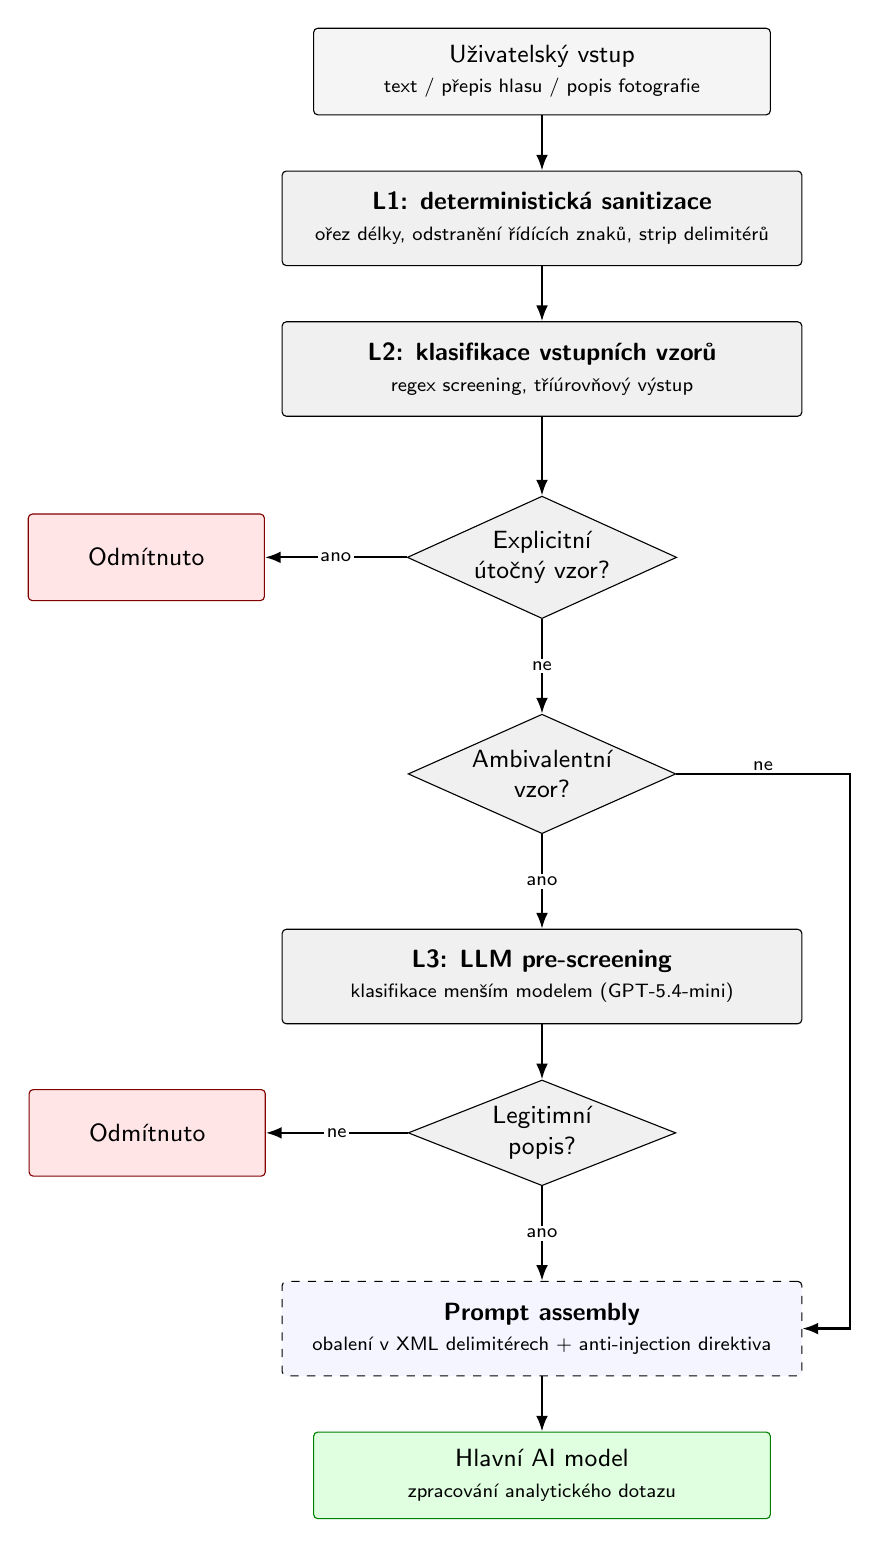
\begin{tikzpicture}[
	font=\small\sffamily,
	node distance=7mm,
	state/.style={
		draw,
		rounded corners=1.5pt,
		minimum height=11mm,
		minimum width=58mm,
		align=center,
		fill=black!4,
	},
	process/.style={
		draw,
		rounded corners=1.5pt,
		minimum height=12mm,
		minimum width=66mm,
		align=center,
		fill=black!6,
	},
	assembly/.style={
		draw,
		dashed,
		rounded corners=1.5pt,
		minimum height=12mm,
		minimum width=66mm,
		align=center,
		fill=blue!4,
	},
	decision/.style={
		draw,
		diamond,
		aspect=2.2,
		minimum height=10mm,
		minimum width=34mm,
		align=center,
		fill=black!6,
		inner sep=1pt,
	},
	rejectbox/.style={state, fill=red!10, draw=red!50!black, minimum width=30mm},
	successbox/.style={state, fill=green!12, draw=green!50!black},
	arr/.style={-{Latex[length=2mm]}, thick},
	lbl/.style={font=\scriptsize\sffamily, midway, fill=white, inner sep=1pt},
]

% --- Hlavní vertikální řetězec ---
\node[state] (input) {Uživatelský vstup\\\scriptsize text / přepis hlasu / popis fotografie};

\node[process, below=of input] (l1) {%
	\textbf{L1: deterministická sanitizace}\\
	{\scriptsize ořez délky, odstranění řídících znaků, strip delimitérů}%
};

\node[process, below=of l1] (l2) {%
	\textbf{L2: klasifikace vstupních vzorů}\\
	{\scriptsize regex screening, tříúrovňový výstup}%
};

\node[decision, below=10mm of l2] (d1) {Explicitní\\útočný vzor?};

\node[decision, below=12mm of d1] (d2) {Ambivalentní\\vzor?};

\node[process, below=12mm of d2] (l3) {%
	\textbf{L3: LLM pre-screening}\\
	{\scriptsize klasifikace menším modelem (GPT-5.4-mini)}%
};

\node[decision, below=of l3] (d3) {Legitimní\\popis?};

\node[assembly, below=12mm of d3] (assembly) {%
	\textbf{Prompt assembly}\\
	{\scriptsize obalení v~XML delimitérech + anti-injection direktiva}%
};

\node[successbox, below=of assembly] (model) {Hlavní AI model\\\scriptsize zpracování analytického dotazu};

% --- Terminální stavy "Odmítnuto" (vlevo) ---
\node[rejectbox, left=18mm of d1] (rej1) {Odmítnuto};
\node[rejectbox, left=18mm of d3] (rej3) {Odmítnuto};

% --- Šipky hlavního toku ---
\draw[arr] (input) -- (l1);
\draw[arr] (l1) -- (l2);
\draw[arr] (l2) -- (d1);
\draw[arr] (d1.south) -- node[lbl] {ne} (d2.north);
\draw[arr] (d2.south) -- node[lbl] {ano} (l3.north);
\draw[arr] (l3.south) -- (d3.north);
\draw[arr] (d3.south) -- node[lbl] {ano} (assembly.north);
\draw[arr] (assembly.south) -- (model.north);

% --- Reject šipky ---
\draw[arr] (d1.west) -- node[lbl] {ano} (rej1.east);
\draw[arr] (d3.west) -- node[lbl] {ne} (rej3.east);

% --- Bypass L3: ne z D2 přeskočí přímo na prompt assembly (vpravo) ---
\coordinate (bypassTop) at ($(d2.east)+(22mm,0)$);
\coordinate (bypassBot) at (bypassTop |- assembly.east);
\draw[arr] (d2.east) -- (bypassTop) -- (bypassBot) -- (assembly.east);
\node[font=\scriptsize\sffamily, fill=white, inner sep=1pt, above]
	at ($(d2.east)!0.5!(bypassTop)$) {ne};

\end{tikzpicture}
}
	\caption{Stavový diagram ochrany proti prompt injection.}
	\label{fig:promptInjection}
\end{figure}

\subsection{Volba poskytovatele a modelu}
\label{subsec:vicePoskytovatelu}

Jako poskytovatel multimodálního jazykového modelu byla zvolena společnost OpenAI, která v~aktuálním kontextu představuje jednu z~nejdostupnějších a~ekosystémově nejstabilnějších platforem se širokou komunitní podporou a~ověřeným strukturovaným JSON výstupem.
Vzhledem k~tomu, že tato práce je tematicky zaměřena na HCI a~nikoliv na vývoj a~trénování modelů umělé inteligence, byl preferován obecný univerzální model před modelem doménově specializovaným.
Lze přepokládat, že model dotrénovaný výhradně na potravinových datech by pro doménu rozpoznávání jídel poskytoval přesnější odhady.
Jeho výměna je však v~rámci zvolené architektury proveditelná bez zásahu do vyšších vrstev aplikace a~představuje přirozený krok před případným nasazením do produkce.

Komunikační vrstva pro analýzu jídel je proto navržena tak, aby byla nezávislá na konkrétním poskytovateli, a to prostřednictvím jednotného abstraktního rozhraní pro generování odpovědí.
V~projektu jsou pro hlavní pipeline připraveny dvě strategie, a~to pro OpenAI Chat Completions a~pro Google Gemini Generative Language.
Zbývající scénáře (analýza cvičení, výpočet nutričních cílů, rozhraní Ask AI) jsou v~aktuální verzi vázány přímo na OpenAI a~rozšíření jejich abstrakce je formulováno jako námět pro další iteraci.

Empirické porovnání tří variant modelů OpenAI (GPT-5.4, GPT-5.4-mini, GPT-5.5) ve dvou iteracích systémového promptu bylo provedeno v~rámci kvantitativního benchmarku popsaného v~sekci~\ref{subsec:benchmarkPresnost}, na jehož základě byl pro produkční nasazení zvolen jako výchozí model GPT-5.4 s~promptem improved v2.

\section{Vstupní modality pro záznam stravy}
\label{sec:vstupniModality}

V~návaznosti na výsledky uživatelské studie (sekce~\ref{sec:uzivatelskaStudie}), která identifikovala potřebu rychlého a flexibilního zápisu jídel v~různých kontextech, implementuje aplikace celkem šest vstupních modalit pro záznam stravy a~doplňkově dvě modality pro záznam cvičení.
Jednotlivé modality jsou volány z~panelu rychlých akcí na hlavní obrazovce a~pokrývají funkční požadavky FR-01, FR-06, FR-11, FR-12, FR-14 a~FR-16.
Modality lze rozdělit do dvou skupin podle způsobu zpracování vstupu: AI-asistované cesty (foto, hlas, text, OCR nutriční etikety a~hlasový vstup pro cvičení) procházejí sdílenou pipeline pro umělou inteligenci a~následně editační obrazovkou, zatímco přímé cesty (čárový kód s~vyhledáním v~databázi Open Food Facts a~manuální zápis jídla i~cvičení) editační obrazovku obcházejí nebo využívají v~upravené podobě.
Tato sekce postupně popisuje implementaci každé z~nich, od plně automatizovaného fotografického vstupu přes hlasový a~textový vstup s~podporou umělé inteligence až po manuální zadání bez asistence umělé inteligence.

\subsection{AI-asistovaný vstup: foto, hlas a text}
\label{subsec:aiVstup}

Trojice modalit s~asistencí umělé inteligence sdílí společnou infrastrukturu: vstup v~podobě obrazu nebo textu je předán do pipeline pro umělou inteligenci a výsledek rozpoznání je prezentován na editační obrazovce jídla (viz obrázek~\ref{fig:screenEditMeal}) zároveň sloužící jako náhled i jako rozhraní pro úpravy.
Modality se liší pouze typem vstupu a uživatelským kontextem, ve kterém jsou volány.

Fotografický vstup (FR-06, FR-12) představuje hlavní inovační prvek aplikace a podporuje dva zdroje obrazu: živý vstup z~kamery prostřednictvím obrazovky skenování a import existujících fotografií z~galerie pomocí knihovny \texttt{image\_picker}.
Uživatel může k~fotografii volitelně přidat krátký textový popis (například \uv{kuřecí salát s~rýží}), který je odeslán společně s~obrazem.
Při prvním použití je zobrazena pětistránková onboardingová sekvence (FR-09) vysvětlující limity rozpoznávání a tipy pro pořízení kvalitního snímku (osvětlení, úhel pohledu, oddělení složek na talíři).
Tato instruktáž zároveň přispívá k~rozlišení mezi limitem modelu a technickou chybou aplikace (FR-10).

Hlasový vstup (FR-14) je realizován samostatnou transkripční službou postavenou nad knihovnou \texttt{speech\_to\_text} s~podporou češtiny a angličtiny podle aktuální lokalizace.
Na obrazovce hlasového vstupu (viz obrázek~\ref{fig:screenVoiceLog}) uživatel zahájí nahrávání stiskem tlačítka, vidí transkripci v~reálném čase a po dokončení ji potvrdí nebo upraví před odesláním do pipeline.
Tok pokrývá záznam jídla i analogický scénář pro záznam cvičení a v~uživatelském testování byl označen za jednu z~nejvíce oceněných funkcí aplikace (viz sekce~\ref{sec:doporuceni}).

Textový vstup (FR-14, FR-11) slouží jako přirozený záložní kanál pro situace, kdy fotografický vstup není praktický nebo selže (jídlo již zkonzumované, omezené podmínky pro focení).
Uživatel popíše jídlo libovolným způsobem v~přirozeném jazyce (například \uv{kuřecí prsa s~rýží a brokolicí, asi 250~gramů}) a vstup prochází stejnou pipeline jako fotografický nebo hlasový.

\subsection{Manuální zadání bez umělé inteligence}
\label{subsec:manualniVstup}

Manuální vstup naplňuje funkční požadavek FR-01 a je určen pro situace, kdy uživatel přesně zná složení jídla a nepotřebuje asistenci umělé inteligence (například domácí vaření s~váhou, balené potraviny s~nutriční etiketou nebo offline režim, kdy není dostupné připojení k~poskytovateli umělé inteligence).
Tok začíná na obrazovce záznamu jídla, která slouží jako sjednocený rozcestník pro výběr existujícího jídla z~historie nebo vytvoření nového záznamu.
V~případě nového záznamu pokračuje uživatel na obrazovku ručního vytvoření nového jídla (viz obrázek~\ref{fig:screenMealLog}), kde vyplní název jídla a postupně přidává jednotlivé ingredience.

Pro každou ingredienci uživatel zadává nutriční hodnoty (kalorie, bílkoviny, sacharidy, tuky) a hmotnost v~gramech nebo počet kusů (FR-15).
Implementace podporuje předvolby porcí (například 100~g, 1~ks, vlastní jednotky) a zobrazování zlomkových hodnot (například 1/2 porce), čímž zjednodušuje zápis běžných situací.
Detail editace ingrediencí probíhá na samostatných obrazovkách editace a detailu ingredience, které sdílí komponenty s~rozhraním pro úpravu výsledku rozpoznání umělou inteligencí.

\subsection{Čtečka čárových kódů}
\label{subsec:carovyKod}

Čtečka čárových kódů naplňuje funkční požadavek FR-16 a je realizována pomocí knihovny \texttt{mobile\_scanner} podporující formáty EAN-8, EAN-13, UPC-A, UPC-E a Code-128.
Po naskenování kódu volá vyhledávací služba klienta veřejné databáze Open Food Facts, který vrací strukturovaný výsledek obsahující název produktu, výrobce a kompletní nutriční hodnoty na 100~g.
Koordinaci skenování, vyhledávání a zobrazení výsledku zajišťuje samostatný kontroler.

V~návaznosti na funkční požadavek FR-10 (rozlišení limitu umělé inteligence a technické chyby aplikace) je v~rámci čárových kódů implementováno šest typů chyb pokrývajících situace jako neexistující kód, produkt nenalezen v~databázi, nepřipojení k~síti, časový limit dotazu, neplatný formát kódu a poškození čtečky.
Každý typ chyby je uživateli prezentován s~konkrétním vysvětlením a doporučením dalšího kroku.
Hlavním omezením této modality je závislost na kompletnosti databáze Open Food Facts, kterou v~uživatelském testování dva ze tří participantů identifikovali jako problematickou pro některé lokální české produkty (viz sekce~\ref{subsec:uiProblemyTesting}).

\subsection{Skenování nutričních etiket}
\label{subsec:nutricniEtikety}

Skenování nutričních etiket představuje doplňkovou modalitu zaměřenou na situace, kdy uživatel má v~ruce balený produkt s~nutriční tabulkou, ale jeho čárový kód není dostupný v~databázi Open Food Facts.
Implementace využívá multimodální schopnosti hlavního modelu umělé inteligence prostřednictvím specializovaného režimu skenování etiket, kdy je obrazovka kamery přepnuta do tohoto režimu a získaný obraz je odeslán do pipeline s~upraveným promptem zaměřeným na extrakci nutričních hodnot z~tabulky.

Aktuální stav implementace pokrývá základní extrakci hodnot pro 100~g produktu (kalorie, bílkoviny, sacharidy, tuky), zatímco rozšířené atributy jako vláknina, sůl nebo vybrané mikronutrienty jsou ponechány jako námět pro budoucí iteraci.
Hlavním omezením modality je rozmanitost vizuálních formátů nutričních etiket napříč značkami a zeměmi, která může vést k~nižší úspěšnosti rozpoznání u~atypicky řešených tabulek.

\section{Implementace klíčových funkcí}
\label{sec:klicoveFunkce}

Tato sekce popisuje implementaci hlavních funkčních celků aplikace, které doplňují vstupní modality popsané v~sekci~\ref{sec:vstupniModality} o~přehledové, analytické, motivační a konfigurační funkce.
Každá podsekce odkazuje na příslušné funkční požadavky z~kapitoly~\ref{ch:navrh} a popisuje konkrétní implementační detaily včetně příslušných obrazovek aplikace.

\subsection{Denní přehled a správa nutričních cílů}
\label{subsec:dennPrehled}

Denní přehled (FR-02) je centrálním prvkem aplikace, který je realizován na hlavní obrazovce (viz obrázek~\ref{fig:screenDashboard}) prostřednictvím dvojice kontrolerů spravujících aktuálně vybraný den.
Kontrolery společně načítají odpovídající denní záznam včetně všech jídel a cvičení a propagují agregované nutriční hodnoty do reaktivních proměnných sledovaných uživatelským rozhraním.

Správa nutričních cílů (FR-03) je centralizována do dedikované služby, která vychází z~Mifflin-St~Jeorovy rovnice doplněné o~uživatelovu úroveň aktivity a cíl (hubnutí, udržení, nabírání).
Cíle jsou perzistovány prostřednictvím repozitáře pro denní záznamy a propagovány na aktuální i budoucí dny.
Konfigurace probíhá na obrazovce nutričních cílů v~profilové sekci (viz obrázek~\ref{fig:screenNutritionGoals}).

\begin{figure}[ht]
	\centering
	\screenshot[width=0.42\textwidth]{figures/screens/ProfileScreen_NutritionGoalsScreen.png}
	\caption{Nastavení nutričních cílů.}
	\label{fig:screenNutritionGoals}
\end{figure}

Doplňkovými funkcemi denního přehledu jsou systém přenosu nevyčerpaných kalorií do následujícího dne (rollover, omezený na nejvýše 500~kcal) a vizualizace plnění cílů v~kalendáři pomocí barevných kruhů znázorňujících podíly jednotlivých makroživin na cíli.
Kalendář na hlavní obrazovce je horizontálně scrollovatelný a umožňuje rychlou navigaci mezi dny bez ztráty kontextu denního přehledu.

\subsection{Správa jídel a ingrediencí}
\label{subsec:spravaJidel}

Správa jídel a ingrediencí (FR-01, FR-13, FR-15) je realizována na editační obrazovce jídla a navazujících obrazovkách pro editaci a detail jednotlivých ingrediencí.
Tyto obrazovky sdílí společnou logiku editace mezi rozpoznanými jídly z~pipeline umělé inteligence i čistě manuálně vytvořenými záznamy, čímž je zajištěna jednotnost uživatelského rozhraní.

Funkce \uv{Fix with AI} (FR-13) umožňuje z~editační obrazovky znovu vyvolat rozpoznání pomocí umělé inteligence s~doplněným kontextem, který uživatel mezitím přidal (například upřesnění typu pokrmu, korekce gramáže nebo poznámka k~jídlu).
Tok je realizován přes samostatnou obrazovku porovnání, která zobrazuje původní a nový výsledek vedle sebe a umožňuje uživateli zvolit, kterou verzi přijmout.

Pro funkci duplikace záznamu jídla na jiný den (FR-18) je implementován modální list s~kalendářovým výběrem dne.
Tento tok byl explicitně požadován respondenty uživatelské studie pro situace, kdy uživatel jí podobné jídlo opakovaně v~průběhu týdne.
Podpora jednotek (FR-15) zahrnuje gramy, 100-gramové porce, vlastní pojmenované jednotky a zobrazení zlomků (například 1/2 porce, 3/4 šálku).

\subsection{Sledování cvičení}
\label{subsec:sledovaniCviceni}

Modul cvičení naplňuje funkční požadavek FR-22 (částečně FR-23) a je realizován dedikovanou obrazovkou (viz obrázek~\ref{fig:screenExerciseLog}), která sjednocuje čtyři způsoby záznamu fyzické aktivity: rozpoznání pomocí umělé inteligence z~textového popisu, hlasový vstup, ruční zadání a výběr ze šablon dříve zaznamenaných cvičení.
Vlastní vstup probíhá na navazující obrazovce, která pro automatickou analýzu textových nebo hlasových popisů využívá centrální pipeline pro umělou inteligenci (viz sekce~\ref{sec:integraceAi}).

Detail jednotlivého záznamu cvičení je dostupný na samostatné obrazovce, doplněné o~modální list pro pokročilé akce (úprava, odstranění, převedení do šablon).
Šablony cvičení jsou modelovány samostatnou entitou v~datovém modelu (viz sekce~\ref{subsec:sablony}) a poskytují uživateli rychlý přístup k~opakovaně používaným aktivitám bez nutnosti opětovného volání umělé inteligence.

Energetický výdej spočítaný z~rozpoznaného nebo zadaného cvičení je propagován do hlavního denního přehledu, kde je zobrazen vedle příjmu energie pro splnění funkčního požadavku FR-22 (příjem versus výdej v~jednom pohledu).

\subsection{Sledování hmotnosti}
\label{subsec:sledovaniHmotnosti}

Sledování tělesné hmotnosti je realizováno samostatným podsystémem nezávislým na denním nutričním cyklu.
Záznam hmotnosti probíhá v~modálním listu (viz obrázek~\ref{fig:screenWeightSheet}), který umožňuje zadání aktuální hodnoty s~volitelnou fotografií dokumentující průběh redukce nebo nárůstu.
Historie záznamů a jejich úprava jsou dostupné na samostatných obrazovkách.

\begin{figure}[ht]
	\centering
	\screenshot[width=0.42\textwidth]{figures/screens/ProgressScreen_WeightBottomSheet.png}
	\caption{Záznam tělesné hmotnosti.}
	\label{fig:screenWeightSheet}
\end{figure}

Perzistenci a reaktivní aktualizace dat zajišťuje samostatný repozitář, který poskytuje vyšším vrstvám aplikace proud záznamů hmotnosti pro vizualizaci.
Karty s~aktuální hodnotou indexu BMI vypočteného podle rovnice~(\ref{eq:bmi}) a s~grafem vývoje hmotnosti za zvolené období jsou součástí obrazovky přehledů (viz obrázek~\ref{fig:screenProgress}).
Modul je propojen s~onboardingem aplikace, kde uživatel zadává počáteční a cílovou hmotnost spolu s~požadovanou rychlostí redukce nebo nárůstu.

\subsection{Oblíbené položky, šablony a historie}
\label{subsec:oblibene}

Rychlost zápisu opakovaných jídel a cvičení (FR-17, FR-18, FR-19), identifikovaná v~uživatelské studii jako klíčový faktor dlouhodobé udržitelnosti, je řešena třemi komplementárními mechanismy.
Oblíbené položky jsou modelovány samostatným příznakem na entitách jídla, ingredience a cvičení a takto označené položky jsou prezentovány v~záložce \uv{Oblíbené} na obrazovce výběru jídla (viz obrázek~\ref{fig:screenMealLog}).
Systém šablon (sekce~\ref{subsec:sablony}) doplňuje oblíbené o~automaticky udržovanou kanonickou verzi opakovaně používaných položek s~metrikou počtu použití pro řazení podle frekvence.
Našeptávání podle historie (FR-19) je realizováno fulltextovým vyhledáváním s~debounce.
Duplikace záznamu na jiný den (FR-18) využívá modální list popsaný v~sekci~\ref{subsec:spravaJidel}.

\subsection{Dietní omezení a vizualizace porušení}
\label{subsec:dietniOmezeni}

Dietní kontext (FR-20) eviduje uživatelská relace ve dvou typech nastavení: předdefinovaný typ diety (vegetariánská, veganská, bezlepková apod.) a vlastní omezení ve volném textovém seznamu.
Při každé analýze jídla je tento kontext zahrnut do promptu pro umělou inteligenci společně s~obrazovým nebo textovým vstupem.
Samotné vyhodnocení, zda rozpoznané jídlo porušuje nastavená uživatelská omezení, je svěřeno modelu, který případnou kolizi označí přímo ve své strukturované odpovědi.
Vizualizace porušení v~kalendáři (FR-21) je realizována kartou na obrazovce přehledů s~měsíční mřížkou a barevně odlišenými dny, kliknutím lze přejít na detailní pohled.

\subsection{Dotazy v~přirozeném jazyce}
\label{subsec:askAi}

Dotazy v~přirozeném jazyce (FR-27) jsou realizovány prostřednictvím dedikované obrazovky a kontroleru (viz obrázek~\ref{fig:screenAskAi}), které poskytují uživateli analytické rozhraní nad jeho historickými nutričními daty.

Implementace využívá dvouprůchodový systém pro snížení nákladů a zlepšení kvality odpovědí.
V~prvním průchodu volá pipeline menší instanci modelu s~úkolem identifikovat časový rozsah dotazu a typ analytické operace (například \uv{minulý týden}, \uv{leden 2026}, \uv{období bez logování}).
Ve druhém průchodu je hlavnímu modelu předán pouze relevantní výřez dat z~lokální databáze prostřednictvím repozitářové vrstvy, čímž se snižuje velikost kontextu a zlepšuje přesnost odpovědi.
Tento návrh umožňuje uživateli pokládat různorodé dotazy od trendů a srovnání období přes detekci vzorců stravování až po doporučení pro úpravu jídelníčku.

\subsection{Notifikace a motivační souhrny}
\label{subsec:notifikace}

Připomínky stravování (FR-28, FR-29) jsou realizovány dedikovanou službou postavenou nad knihovnou \texttt{flutter\_local\_notifications}, která plánuje notifikace s~ohledem na aktuální časové pásmo zařízení.
Aplikace nabízí pět typů stravovacích připomínek (snídaně, svačina, oběd, odpolední svačina, večeře) doplněných o~volitelné závěrečné shrnutí dne.
Jejich časy a aktivaci uživatel konfiguruje na samostatné obrazovce nastavení (viz obrázek~\ref{fig:screenReminders}).

Doplňkovou funkcí je generování motivačních souhrnů (FR-28), které periodicky analyzují data uživatele (denně, týdně, měsíčně) a prostřednictvím modelu umělé inteligence vytvářejí krátké personalizované shrnutí jako pozitivní zpětnou vazbu pro dlouhodobé cíle.
Souhrny jsou zobrazovány v~modálním listu (viz obrázek~\ref{fig:screenMotivationalSummary}).

\begin{figure}[ht]
	\centering
	\begin{minipage}[t]{0.31\textwidth}
		\centering
		\screenshot[width=\textwidth]{figures/screens/ProfileScreen_TrackingRemindersScreen.png}
		\\(a)~Přehled připomínek
	\end{minipage}\hfill
	\begin{minipage}[t]{0.31\textwidth}
		\centering
		\screenshot[width=\textwidth]{figures/screens/ProfileScreen_TrackingReminders_BottomSheet.png}
		\\(b)~Nastavení času
	\end{minipage}\hfill
	\begin{minipage}[t]{0.31\textwidth}
		\centering
		\screenshot[width=\textwidth]{figures/screens/MotivationalSummaryScreen_BottomSheet.png}
		\\(c)~Motivační souhrn
	\end{minipage}
	\caption{Notifikace a motivační souhrny.}
	\label{fig:screenReminders}
	\label{fig:screenMotivationalSummary}
\end{figure}

\subsection{Export dat a sdílení}
\label{subsec:exportDat}

Export dat (FR-25) podporuje dva výstupní formáty: tabulkový CSV pro další zpracování v~externích nástrojích a formátovaný PDF report pro archivaci nebo sdílení s~odborníkem na výživu.
Tok exportu začíná na úvodní obrazovce (viz obrázek~\ref{fig:screenExport}), kde uživatel zvolí formát, časový rozsah a obsah, a pokračuje na navazujících obrazovkách pro detailní konfiguraci PDF výstupu.

\begin{figure}[ht]
	\centering
	\begin{minipage}[t]{0.42\textwidth}
		\centering
		\screenshot[width=\textwidth]{figures/screens/ExportSummaryReportScreen.png}
		\\(a)~Konfigurace exportu
	\end{minipage}\hfill
	\begin{minipage}[t]{0.42\textwidth}
		\centering
		\screenshot[width=\textwidth]{figures/screens/ExportSummaryReportScreenExport.png}
		\\(b)~Vygenerovaný export
	\end{minipage}
	\caption{Tok exportu dat.}
	\label{fig:screenExport}
\end{figure}

Sdílení individuálních záznamů jídla je realizováno samostatnou službou nad knihovnou \texttt{share\_plus}, která prostřednictvím systémového dialogu distribuuje snímek jídla nebo strukturovaný textový záznam.

\subsection{Integrace se zdravotními platformami}
\label{subsec:zdravotniIntegrace}

Integrace s~Apple Health (iOS) a Health Connect (Android) je realizována dedikovanou službou nad knihovnou \texttt{health}, která poskytuje jednotné API pro čtení a zápis zdravotních dat napříč oběma platformami.
Konfigurace integrace probíhá na samostatné obrazovce v~profilové sekci (viz obrázek~\ref{fig:screenHealthIntegration}).

\begin{figure}[ht]
	\centering
	\screenshot[width=0.42\textwidth]{figures/screens/ProfileScreen_SyncAppleHealthScreen.png}
	\caption{Integrace se zdravotními platformami.}
	\label{fig:screenHealthIntegration}
\end{figure}

Načtené údaje o~spálených kaloriích jsou promítány do denního přehledu.
Samostatný atribut zdroje odlišuje manuálně zadaná cvičení od importovaných.
Uživatel má prostřednictvím samostatných přepínačů kontrolu nad tím, zda a jak se importovaný energetický výdej promítá do denního kalorického limitu a zda se nevyčerpané kalorie přenášejí do následujícího dne.
Aktuální implementace neobsahuje granulární multiplikátory pro různé typy aktivit (FR-23 částečně, viz sekce~\ref{sec:omezeniImplementace}).

\subsection{Lokalizace, onboarding a profil uživatele}
\label{subsec:lokalizaceOnboarding}

Lokalizace aplikace (čeština, angličtina) je realizována knihovnou \texttt{easy\_localization} s~automaticky generovanými klíči a JSON překladovými soubory v~adresáři s~assets.
Onboardingový tok (FR-04, částečně FR-09 a FR-30) zahrnuje jedenáct obrazovek včetně volitelné obrazovky \uv{Custom Diet} pro vyplnění vlastních dietních preferencí a provází nového uživatele od zadání základních údajů přes volbu cíle a výpočet doporučených kalorií až po uložení prvního denního záznamu.
Profilová obrazovka osobních údajů a obrazovka předvoleb aplikace (viz obrázek~\ref{fig:screenPersonalDetailsAndPrefs}) slouží jako primární rozhraní pro pozdější úpravu profilu a doplňková nastavení.

\begin{figure}[ht]
	\centering
	\begin{minipage}[t]{0.42\textwidth}
		\centering
		\screenshot[width=\textwidth]{figures/screens/ProfileScreen_PersonalDetailsScreen.png}
		\\(a)~Osobní údaje
	\end{minipage}\hfill
	\begin{minipage}[t]{0.42\textwidth}
		\centering
		\screenshot[width=\textwidth]{figures/screens/ProfileScreen_Preferences.png}
		\\(b)~Předvolby aplikace
	\end{minipage}
	\caption{Profilové obrazovky aplikace.}
	\label{fig:screenPersonalDetailsAndPrefs}
\end{figure}

Atributy uživatelské relace jsou perzistovány prostřednictvím dedikované služby nad klíč-hodnota úložištěm.
FR-30 (skrytí nebo zobrazení pokročilých funkcí) je implementován individuálními přepínači v~předvolbách (přebírání spálených kalorií, přenos nevyčerpaných kalorií, automatická úprava makroživin), bez explicitního režimu \emph{basic} versus \emph{advanced}.

\subsection{Další implementované funkce}
\label{subsec:dalsiFunkce}

Vedle hlavních funkcí pokrývajících funkční požadavky obsahuje aplikace několik doplňkových mechanismů, které vznikly v~průběhu implementace na základě praktických potřeb a zpětné vazby z~průběžného testování.

Sledování série po sobě jdoucích dnů se záznamy je realizováno samostatným podsystémem, který udržuje aktuální a nejdelší dosaženou sérii a zobrazuje je v~motivačním dialogu při dosažení významných milníků.
Tato funkce slouží jako pozitivní zpětná vazba v~návaznosti na zjištění z~uživatelské studie, kde respondenti opakovaně zmiňovali význam motivačních prvků pro dlouhodobou udržitelnost.

Aplikace dále podporuje widgety na domovské obrazovce zařízení prostřednictvím dedikované synchronizační vrstvy a směrovače akcí, které umožňují uživateli vidět denní souhrn kalorií a otevřít konkrétní vstupní modalitu bez nutnosti spouštět aplikaci.
Vizualizace plnění cílů v~kalendáři využívá vlastní renderování kruhových indikátorů pro každý den, kde tloušťka jednotlivých kruhů odráží podíl jednotlivých makroživin na cíli.

Pro zlepšování kvality rozpoznávání pomocí umělé inteligence je k~dispozici funkce hlášení nesprávně rozpoznaného jídla, která sbírá uživatelskou zpětnou vazbu pro budoucí ladění promptů.
Funkce automatické úpravy makroživin proporcionálně přepočítává cíle pro bílkoviny, sacharidy a tuky při změně kalorického cíle, čímž odstiňuje uživatele od ručního dopočítávání podílů.

Z~hlediska funkčního požadavku FR-05 (kontrola nad daty) aplikace umožňuje mazání jednotlivých záznamů jídel a cvičení, neobsahuje však úplné mazání uživatelského profilu.
Funkční požadavek FR-26 (offline tolerance) je naplněn principem \emph{local-first}, kdy jsou veškerá uživatelská data primárně ukládána do lokální SQLite databáze (viz sekce~\ref{sec:datovyModel}), což zajišťuje plnou funkčnost aplikace bez internetového připojení s~výjimkou modalit závislých na cloudovém modelu umělé inteligence.

\section{Přehled implementovaných funkčních požadavků}
\label{sec:prehledFR}

Pro shrnutí míry pokrytí návrhové specifikace je v~tabulce~\ref{tab:fr-status} uveden přehled stavu implementace všech třiceti funkčních požadavků definovaných v~sekci~\ref{sec:pozadavky}.
Každý požadavek je klasifikován do jedné ze tří kategorií, kterými jsou implementováno, částečně implementováno a neimplementováno, doplněných o~stručné zdůvodnění a odkaz na příslušné komponenty aplikace.
Tato klasifikace tvoří přímý podklad pro vyhodnocení splnění návrhových cílů v~kapitole~\ref{ch:zaver} a pro identifikaci oblastí, jejichž ověření je předmětem uživatelského testování v~kapitole~\ref{ch:testovani}.

\begin{table}[ht]
	\centering
	\caption{Stav implementace funkčních požadavků.}
	\label{tab:fr-status}
	\small
	\begin{tabular}{p{1.1cm}p{5.5cm}p{2.6cm}p{5cm}}
		\toprule
		\textbf{FR} & \textbf{Název} & \textbf{Stav} & \textbf{Poznámka} \\
		\midrule
		FR-01 & Ruční přidání záznamu jídla bez umělé inteligence & Implementováno & Editační obrazovka jídla, manuální vstup ingrediencí \\
		FR-02 & Denní přehled kalorií a makroživin & Implementováno & Hlavní obrazovka s~kontrolery denního záznamu \\
		FR-03 & Nastavení cílových hodnot & Implementováno & Služba nutričních cílů s~obrazovkou nastavení \\
		FR-04 & Správa profilu uživatele & Implementováno & Profilové obrazovky, služba uživatelské relace \\
		FR-05 & Kontrola nad daty a mazání & Částečně implementováno & Mazání jídel a cvičení funkční, mazání účtu chybí \\
		FR-06 & Fotografie jako vstup pro rozpoznání & Implementováno & Obrazovka kamery, pipeline umělé inteligence \\
		FR-07 & Návrh položek a porcí umělou inteligencí & Implementováno & \texttt{AiPipelineService}, strukturovaný JSON prompt \\
		FR-08 & Indikace nejistoty výstupu & Implementováno & Barevný badge (zelená $\geq$ 75~\%, žlutá $\geq$ 50~\%, červená $<$ 50~\%) \\
		FR-09 & Vysvětlení limitů umělé inteligence & Implementováno & Pětistránková onboardingová sekvence s~tipy \\
		FR-10 & Rozlišení limitu umělé inteligence a technické chyby & Částečně implementováno & Čárový kód: 6 typů chyb, AI pipeline: generické selhání \\
		FR-11 & Textový fallback po selhání rozpoznání & Implementováno & Textový popis $\to$ pipeline umělé inteligence \\
		FR-12 & Import fotografie z~galerie & Implementováno & Integrace knihovny \texttt{image\_picker} \\
		FR-13 & Opakování rozpoznání z~editace & Implementováno & \uv{Fix with AI} a samostatná obrazovka porovnání verzí \\
		FR-14 & Záznam bez fotografie (hlas, text) & Implementováno & Hlasový vstup, textový popis, manuální vstup \\
		FR-15 & Jednotky množství (gramy, kusy) & Implementováno & 1~g, 100~g, vlastní jednotky, zlomky \\
		FR-16 & Čtečka čárových kódů & Implementováno & Knihovna \texttt{mobile\_scanner}, klient Open Food Facts \\
		FR-17 & Oblíbené položky & Implementováno & Příznak na jídlech, ingrediencích a cvičeních \\
		FR-18 & Duplikace předchozího záznamu & Implementováno & Modální list s~výběrem data \\
		FR-19 & Našeptávání podle historie & Částečně implementováno & Fulltextové vyhledávání s~debounce, bez klasického dropdown \\
		FR-20 & Dietní omezení a intolerance & Implementováno & Předdefinovaný typ diety + uživatelská omezení \\
		FR-21 & Porušení dietních omezení v~kalendáři & Implementováno & Karta s~měsíční mřížkou na obrazovce přehledů \\
		FR-22 & Příjem versus výdej v~jednom pohledu & Implementováno & Hlavní obrazovka s~kalorickým příjmem a výdajem \\
		FR-23 & Nastavení integrace výdeje & Částečně implementováno & Přepínače pro výdej a rollover, bez granulárních multiplikátorů \\
		FR-24 & Týdenní a měsíční přehledy & Implementováno & Obrazovka přehledů s~kartou týdenní energie \\
		FR-25 & Export dat (CSV, PDF) & Implementováno & Dedikovaná služba exportu s~výběrem období \\
		FR-26 & Offline tolerance & Implementováno & Lokální SQLite, umělá inteligence vyžaduje připojení \\
		FR-27 & Dotazy v~přirozeném jazyce & Implementováno & Obrazovka Ask AI, dvouprůchodový systém \\
		FR-28 & Měsíční motivační souhrn & Implementováno & Periodicky generované shrnutí (denně, týdně, měsíčně) \\
		FR-29 & Nastavitelné notifikace & Implementováno & Pět typů připomínek s~knihovnou \texttt{flutter\_local\_notifications} \\
		FR-30 & Skrytí a zobrazení pokročilých funkcí & Částečně implementováno & Individuální přepínače, bez režimu basic versus advanced \\
		\bottomrule
	\end{tabular}
\end{table}

\section{Omezení implementace}
\label{sec:omezeniImplementace}

Aplikace Foody představuje funkční prototyp ověřující navržený koncept a v~několika oblastech nedosahuje plného potenciálu návrhu z~kapitoly~\ref{ch:navrh}.
Tato sekce shrnuje hlavní omezení výsledné implementace, která je třeba zohlednit při interpretaci výsledků uživatelského testování v~kapitole~\ref{ch:testovani} a při formulaci doporučení pro další rozvoj v~kapitole~\ref{ch:zaver}.

Hlavní omezení vyplývá z~povahy rozpoznávání pomocí umělé inteligence.
Multimodální jazykový model dosahuje vyšší přesnosti u~jednoznačně viditelných pokrmů, zatímco u~složených jídel s~překrývajícími se ingrediencemi a u~regionálně specifických receptur klesá spolehlivost odhadu.
Kvalita rozpoznání je rovněž závislá na kvalitě vstupního obrazu, zejména na osvětlení a úhlu pohledu, což aplikace adresuje pětistránkovou onboardingovou instruktáží (FR-09), nemůže však zcela kompenzovat nepříznivé pořizovací podmínky.
Latence rozpoznávání se v~kontrolovaných podmínkách pohybuje hluboko pod stanoveným limitem 20~vteřin (NFR-02), avšak energetický odhad zůstává aproximací s~nejistotou, kterou aplikace transparentně signalizuje prostřednictvím tříúrovňového indikátoru spolehlivosti.

Architektura aplikace závisí na třech externích službách, jejichž dostupnost ovlivňuje uživatelskou zkušenost.
Komunikace s~poskytovatelem modelu umělé inteligence vyžaduje aktivní internetové připojení, takže funkce rozpoznávání jídel z~fotografie, hlasového a textového popisu, analýzy cvičení a dotazů v~přirozeném jazyce nejsou v~režimu offline dostupné, zatímco zbývající funkcionality jsou plně funkční lokálně (FR-26).
Vyhledávání podle čárového kódu se opírá o~veřejnou databázi Open Food Facts, jejíž pokrytí lokálních českých produktů není úplné, což bylo identifikováno jako omezení i v~uživatelském testování (sekce~\ref{subsec:uiProblemyTesting}).
Provoz multimodálního modelu představuje nezanedbatelný náklad na volání API, jehož výše je úměrná frekvenci použití funkcí postavených na umělé inteligenci a v~současné implementaci není limitován kvótami na úrovni uživatele.

Pět funkčních požadavků (FR-05, FR-10, FR-19, FR-23 a FR-30) bylo implementováno pouze částečně.
Konkrétní povaha omezení jednotlivých požadavků je uvedena ve sloupci \emph{Poznámka} tabulky~\ref{tab:fr-status} v~sekci~\ref{sec:prehledFR}.

Z~technických omezení je v~současné implementaci skenování nutričních etiket pokryto pouze pro základní makroživiny, zatímco rozšířené atributy jako vláknina, sůl a vybrané mikronutrienty zůstávají námětem pro budoucí iteraci.
Analýza cvičení a výpočet nutričních cílů jsou v~aktuální verzi vázány přímo na poskytovatele OpenAI a nepřepínají se spolu s~hlavním poskytovatelem rozpoznávání jídel.
Ověření kompatibility Gemini API pro tyto scénáře nebylo v~rámci práce dokončeno.
Aplikace dále neobsahuje automatický fallback mezi poskytovateli při selhání jednoho z~nich a nedisponuje cloudovou synchronizací ani vzdálenou zálohou dat, což odpovídá zvolenému architektonickému přístupu bez vlastního backendu.

Posledním okruhem omezení je rozsah uživatelského testování.
Implementace byla ověřena na malém vzorku tří participantů v~kontrolovaném prostředí, jak je popsáno v~kapitole~\ref{ch:testovani}, což odpovídá rozsahu kvalitativního testování v~rámci diplomové práce, ale neumožňuje zobecnění výsledků na širší populaci.
Dlouhodobá retence uživatelů, přesnost odhadů v~reálném používání a chování aplikace v~produkčním prostředí na různých zařízeních a operačních systémech zůstávají předmětem dalšího ověření, jež je formulováno jako doporučení pro budoucí validační studii v~sekci~\ref{sec:doporuceni}.

\chapter{Testování}
\label{ch:testovani}

Tato kapitola popisuje průběh a výsledky uživatelského testování aplikace Foody.
Cílem testování bylo ověřit použitelnost implementované aplikace na reálných uživatelích a identifikovat případné problémy v~uživatelském rozhraní a interakčních tocích.
V~první části kapitoly je popsána zvolená metodika, výběr participantů, sada testovacích úloh a použité dotazníky.
Následně jsou prezentovány výsledky plnění jednotlivých úloh, výstupy standardizovaných dotazníků a identifikované problémy s~doporučeními pro další iteraci vývoje.

\section{Metodika testování}
\label{sec:metodikaTestovani}

V~rámci testování aplikace Foody byla zvolena kombinace metody \emph{think aloud} a úlohového testování (\emph{task-based usability testing}).
Tato kombinace umožňuje získat jak kvantitativní data o~úspěšnosti a rychlosti plnění úloh, tak kvalitativní poznatky o~kognitivních procesech participantů při interakci s~aplikací.
Následující podkapitoly popisují výběr participantů, prostředí testování, sadu testovacích úloh a použité dotazníky a metriky.

\subsection{Výběr a charakteristika participantů}
\label{subsec:vyberParticipantu}

Pro uživatelské testování byli vybráni celkem čtyři participanti, kteří představují různé uživatelské profily z~hlediska zkušeností se sledováním stravy a technologické zdatnosti.
Tento počet je v~souladu s~doporučeními Nielsena, podle kterých pět participantů odhalí přibližně 80~\% problémů použitelnosti, přičemž již čtyři participanti pokrývají většinu kritických nedostatků~\cite{nielsen2000fiveUsers}.
Participanti byli vybráni s~ohledem na variabilitu věku, pohlaví a předchozích zkušeností s~aplikacemi pro sledování kalorického příjmu, čímž bylo zajištěno pokrytí rozdílných uživatelských perspektiv.

% TODO: doplnit profily participantů P1--P4 (jedná se o stejné participanty jako v uživatelské studii v sekci 3.2.2).
% Pro každého uvést primární cíl, zkušenosti s calorie tracking aplikacemi a technologickou zdatnost (2--4 věty).
% Vzor: „P1 (žena, 28 let) se aktivně věnuje fitness a sledování stravy. Dříve používala MyFitnessPal po dobu šesti měsíců,
% kterou opustila kvůli časové náročnosti manuálního zápisu. Od testované aplikace očekává rychlejší záznam díky AI rozpoznávání."

\subsection{Prostředí a průběh testovací relace}
\label{subsec:prostrediRelace}

Testování probíhalo formou individuálních relací v~kontrolovaném prostředí, kdy každý participant pracoval s~aplikací na reálném mobilním zařízení.
V~průběhu testování byla použita metoda souběžného protokolu \emph{think aloud}, při které participanti verbalizovali své myšlenky, dojmy a pochybnosti během plnění úloh~\cite{nielsen1994thinkAloud}.
Na začátku každé relace byl participant seznámen s~účelem testování, podepsal informovaný souhlas a obdržel instrukce k~verbalizaci myšlenek.

Každá testovací relace měla odhadovanou délku 75 až 90~minut a sestávala ze čtyř fází, jejichž přehled je uveden v~tabulce~\ref{tab:strukturaRelace}.
V~úvodní fázi (přibližně 5~minut) byl participant seznámen s~průběhem testu a instrukcemi k~metodě \emph{think aloud}.
Hlavní fáze testování (60 až 70~minut) zahrnovala plnění třinácti testovacích úloh, přičemž po dokončení každé úlohy participant vyplnil dotazník SEQ.
Třetí fáze (přibližně 10~minut) byla věnována vyplnění standardizovaných dotazníků SUS a UEQ-S hodnotících celkovou zkušenost s~aplikací.
Závěrečná fáze (5 až 10~minut) sestávala z~polostrukturovaného debriefingu s~šesti otevřenými otázkami zaměřenými na celkový dojem, pozitivní a negativní aspekty aplikace, srovnání s~konkurenčními řešeními a ochotu k~pravidelnému používání.

\begin{table}[ht]
	\centering
	\caption{Struktura testovací relace.}
	\label{tab:strukturaRelace}
	\begin{tabular}{lll}
		\toprule
		\textbf{Fáze} & \textbf{Délka} & \textbf{Obsah} \\
		\midrule
		Úvod & 5~min & Představení, souhlas, instrukce k~\emph{think aloud} \\
		Testovací úlohy & 60--70~min & Plnění úloh T1--T13 s~SEQ po každé úloze \\
		Dotazníky & 10~min & SUS a UEQ-S \\
		Debriefing & 5--10~min & Otevřené otázky, celkový dojem \\
		\bottomrule
	\end{tabular}
\end{table}

Na základě přípravy testovacího prostředí byla na zařízení nainstalována čistá verze aplikace bez předchozích dat, čímž byl simulován stav prvního spuštění.
Do galerie zařízení byly nahrány připravené fotografie jídel pro úlohu T3, na stůl bylo připraveno reálné jídlo pro úlohu T2 a balený produkt s~čárovým kódem pro úlohu T6.
Průběh testování byl zaznamenáván formou záznamu obrazovky a zvukového záznamu pro následnou analýzu verbalizací.

\subsection{Testovací úlohy}
\label{subsec:testovaciUlohy}

Testovací úlohy byly navrženy tak, aby pokrývaly klíčové funkční požadavky a případy užití definované v~kapitole~\ref{ch:navrh} (viz sekce~\ref{sec:uzivatelskaStudie}).
Úlohy jsou seřazeny v~pořadí, které simuluje přirozený průchod aplikací od prvního spuštění přes různé způsoby záznamu jídla až po přehledy a export dat.
Celkem bylo definováno třináct testovacích úloh, jejichž přehled včetně vazby na funkční požadavky a případy užití je uveden v~tabulce~\ref{tab:ulohy}.

\begin{table}[ht]
	\centering
	\caption{Přehled testovacích úloh s~vazbou na funkční požadavky a případy užití.}
	\label{tab:ulohy}
	\begin{tabular}{cll}
		\toprule
		\textbf{Úloha} & \textbf{Název} & \textbf{Pokryté FR / UC} \\
		\midrule
		T1 & Onboarding a nastavení profilu & FR-03, FR-04, FR-20, UC07 \\
		T2 & Záznam jídla z~fotografie & FR-06, FR-07, FR-08, FR-09, UC01 \\
		T3 & Import fotografie z~galerie & FR-12 \\
		T4 & Oprava výsledku rozpoznání a re-analýza & FR-11, FR-13, UC02 \\
		T5 & Záznam jídla hlasem & FR-14 \\
		T6 & Skenování čárového kódu & FR-16, UC04 \\
		T7 & Ruční přidání záznamu & FR-01, FR-15, UC03 \\
		T8 & Oblíbené a duplikace jídla & FR-17, FR-18, UC05 \\
		T9 & Záznam cvičení hlasem & --- \\
		T10 & Zaznamenání váhy & --- \\
		T11 & Denní přehled a smazání záznamu & FR-02, FR-05, FR-22 \\
		T12 & Týdenní přehled a Ask AI & FR-24, FR-27, UC08 \\
		T13 & Export dat & FR-25 \\
		\bottomrule
	\end{tabular}
\end{table}

Úloha T1 zahrnovala kompletní onboarding flow aplikace, v~rámci kterého participant zadal základní údaje (váha, výška, věk), nastavil kalorický cíl a zvolil případné dietní preference.
Úlohy T2 až T6 pokrývaly jednotlivé vstupní modality pro záznam jídla, konkrétně fotografii z~kamery (T2), import z~galerie (T3), opravu a re-analýzu výsledku rozpoznání (T4), hlasový vstup (T5) a skenování čárového kódu (T6).
Úloha T7 testovala ruční přidání záznamu bez využití umělé inteligence, zatímco úloha T8 ověřovala práci s~oblíbenými položkami a funkcí kopírování jídla na jiný den.

V~rámci úloh T9 a T10 bylo testováno rozšíření aplikace nad rámec původní specifikace, konkrétně záznam cvičení hlasovým vstupem a zaznamenání tělesné váhy.
Úlohy T11 až T13 se zaměřovaly na přehledové a analytické funkce aplikace, včetně denního přehledu se smazáním záznamu (T11), týdenního přehledu s~funkcí Ask AI pro dotazy v~přirozeném jazyce (T12) a exportu dat (T13).

Z~celkového počtu třiceti funkčních požadavků definovaných v~kapitole~\ref{ch:navrh} je testovacími úlohami přímo pokryto dvacet dva požadavků, což představuje 73~\% specifikace.
Všech osm případů užití (UC01 až UC08) je pokryto alespoň jednou úlohou.
Zbývajících osm funkčních požadavků nebylo zahrnuto do testování z~důvodů, které jsou shrnuty v~tabulce~\ref{tab:nepokrytaFR}.

\begin{table}[ht]
	\centering
	\caption{Funkční požadavky nepokryté testovacími úlohami s~uvedením důvodu.}
	\label{tab:nepokrytaFR}
	\small
	\begin{tabular}{p{1.1cm}p{4.5cm}p{8cm}}
		\toprule
		\textbf{FR} & \textbf{Název} & \textbf{Důvod vynechání} \\
		\midrule
		FR-10 & Rozlišení chyb rozpoznávání a aplikace & Nelze spolehlivě vyvolat v~kontrolovaném prostředí \\
		FR-19 & Našeptávání názvů & Implicitně pokryto vyhledáváním v~úlohách T7 a T8 \\
		FR-21 & Porušení diet v~kalendáři & Vyžaduje historická data s~porušeními, obtížné simulovat \\
		FR-23 & Nastavení integrace výdeje & Pouze přepínač v~nastavení, nízká interakční hodnota \\
		FR-26 & Offline tolerance & Vyžaduje odpojení od sítě během testu \\
		FR-28 & Motivační souhrn & Vyžaduje dlouhodobý cyklus (denní, týdenní, měsíční) \\
		FR-29 & Konfigurovatelné notifikace & Efekt vyžaduje časový odstup \\
		FR-30 & Zobrazení a skrytí pokročilých funkcí & Pouze přepínače v~nastavení, nízká interakční hodnota \\
		\bottomrule
	\end{tabular}
\end{table}

Během plnění vybraných úloh bylo současně pozorováním ověřováno plnění nefunkčních požadavků.
V~rámci úlohy T2 byla měřena latence rozpoznávání umělou inteligencí (NFR-02, limit 20~s) časem od odeslání fotografie do zobrazení výsledku.
Počet kroků potřebných pro zápis jídla (NFR-03, limit 6~kroků) byl zaznamenáván při úlohách T2, T5, T6 a T7.
Čas zápisu (NFR-04) byl měřen pro nový záznam v~úloze T2 (limit 5~minut) a pro opakovaný záznam v~úloze T8 (limit 1~minuta).

\subsection{Použité dotazníky a metriky}
\label{subsec:dotazniky}

Pro kvantitativní hodnocení použitelnosti a uživatelské zkušenosti byly v~rámci testování použity tři standardizované dotazníky.
Výběr nástrojů pokrývá hodnocení na úrovni jednotlivých úloh (SEQ), celkovou použitelnost systému (SUS) a uživatelskou zkušenost v~pragmatické i hedonické dimenzi (UEQ-S).
Společné použití těchto tří dotazníků umožňuje triangulaci výsledků a poskytuje komplexní pohled na kvalitu interakce uživatele s~aplikací.

Bezprostředně po dokončení každé testovací úlohy participant vyplnil dotazník \emph{Single Ease Question} (SEQ), který sestává z~jediné otázky hodnotící subjektivní obtížnost úlohy na sedmibodové škále, kde 1 znamená „velmi obtížná" a 7 „velmi snadná"~\cite{sauro2009seq}.
Výhodou SEQ je minimální zatížení participanta a možnost okamžitého zachycení dojmu z~právě dokončené úlohy, aniž by byl narušen průběh testování.
Na základě dostupných benchmarků je za dobré hodnocení považován průměr SEQ skóre 5,5 a vyšší.

Po dokončení všech testovacích úloh participant vyplnil dotazník \emph{System Usability Scale} (SUS), který představuje standardizovaný nástroj pro hodnocení celkové použitelnosti systému~\cite{brooke1996sus}.
Dotazník SUS sestává z~deseti položek hodnocených na pětibodové Likertově škále (1~--~rozhodně nesouhlasím, 5~--~rozhodně souhlasím), přičemž liché položky jsou formulovány pozitivně a sudé negativně.
Výsledné skóre se pohybuje v~rozsahu 0 až 100~bodů a vypočítá se podle vzorce~(\ref{eq:sus}).
V~kontextu dostupných benchmarků odpovídá průměrné SUS skóre napříč studiemi přibližně 68~bodům, přičemž skóre nad 80,3~bodu řadí systém mezi horních 10~\% hodnocených aplikací~\cite{bangor2008susAdjective}.

\begin{equation}
	\mathrm{SUS} = \bigl((S_L - 5) + (25 - S_S)\bigr) \cdot 2{,}5,
	\label{eq:sus}
\end{equation}

\noindent kde $S_L$ je součet odpovědí na lichých položkách (1, 3, 5, 7, 9) a $S_S$ je součet odpovědí na sudých položkách (2, 4, 6, 8, 10).

Jako doplňkový nástroj pro hodnocení uživatelské zkušenosti byl použit dotazník \emph{User Experience Questionnaire Short} (UEQ-S), který měří pragmatickou a hedonickou kvalitu systému prostřednictvím osmi položek~\cite{schrepp2017ueqs}.
Každá položka má formu sémantického diferenciálu na sedmibodové škále ($-3$ až $+3$), přičemž záporný pól je vždy umístěn na levé straně.
Položky 1 až 4 (bránící/podporující, složitý/jednoduchý, neefektivní/efektivní, matoucí/jasný) měří pragmatickou kvalitu a položky 5 až 8 (nudný/vzrušující, nezajímavý/zajímavý, obvyklý/vynalézavý, tradiční/moderní) měří hedonickou kvalitu.
Pragmatická kvalita se vypočítá jako průměr položek 1 až 4, hedonická kvalita jako průměr položek 5 až 8 a celkové skóre jako průměr všech osmi položek.
Byla použita oficiální česká verze dotazníku validovaná a dostupná na stránkách projektu UEQ.

\section{Výsledky testování}
\label{sec:vysledkyTestovani}

Následující podkapitoly prezentují výsledky uživatelského testování v~členění na kvantitativní údaje o~plnění jednotlivých úloh, hodnocení SEQ a výstupy standardizovaných dotazníků SUS a UEQ-S.
Výsledky jsou doplněny o~kvalitativní poznatky získané analýzou verbalizací participantů v~průběhu metody \emph{think aloud} a z~odpovědí debriefingových rozhovorů.

\subsection{Plnění úloh a hodnocení SEQ}
\label{subsec:plneniUloh}

% TODO: pro každou úlohu T1--T13 uvést v průvodním textu:
%   --- míra dokončení (kolik ze 4 participantů úspěšně dokončilo)
%   --- průměrný čas plnění
%   --- počet kritických chyb (participant nedokázal pokračovat bez pomoci moderátora)
%   --- průměrné SEQ skóre
%   --- reprezentativní pozorování z think aloud (parafráze, ne přímé citáty)
% Doporučený rozsah: 1--2 odstavce na úlohu; výrazné nálezy rozepsat (T2, T4, T5, T8),
% bezproblémové úlohy lze sloučit do souhrnného odstavce.

\begin{table}[ht]
	\centering
	\caption{Výsledky plnění testovacích úloh a hodnocení SEQ.}
	\label{tab:vysledkyUloh}
	\begin{tabular}{cccccc}
		\toprule
		\textbf{Úloha} & \textbf{Dokončení (n/4)} & \textbf{$\varnothing$ čas (s)} & \textbf{Kritické chyby} & \textbf{$\varnothing$ SEQ (1--7)} \\
		\midrule
		T1 & TODO & TODO & TODO & TODO \\
		T2 & TODO & TODO & TODO & TODO \\
		T3 & TODO & TODO & TODO & TODO \\
		T4 & TODO & TODO & TODO & TODO \\
		T5 & TODO & TODO & TODO & TODO \\
		T6 & TODO & TODO & TODO & TODO \\
		T7 & TODO & TODO & TODO & TODO \\
		T8 & TODO & TODO & TODO & TODO \\
		T9 & TODO & TODO & TODO & TODO \\
		T10 & TODO & TODO & TODO & TODO \\
		T11 & TODO & TODO & TODO & TODO \\
		T12 & TODO & TODO & TODO & TODO \\
		T13 & TODO & TODO & TODO & TODO \\
		\bottomrule
	\end{tabular}
\end{table}

% TODO: souhrnná interpretace výsledků z tabulky:
%   --- které úlohy měly nejvyšší a nejnižší SEQ skóre
%   --- kde se vyskytly kritické chyby a co je způsobilo
%   --- celkový průměr SEQ napříč úlohami a srovnání s benchmarkem 5,5
%   --- výsledky ověření NFR-02 (latence), NFR-03 (počet kroků), NFR-04 (čas zápisu)
%   --- shrnutí, které toky fungují dobře a které vyžadují pozornost.

\subsection{Výsledky System Usability Scale}
\label{subsec:vysledkySus}

% TODO: interpretace SUS výsledků. Vzor:
% „Průměrné SUS skóre aplikace Foody činilo X,X bodu (SD = X,X), což ji řadí do kategorie X
% podle adjektivní stupnice Bangor a kol. Nejvyšší hodnocení získala položka č. X (průměr X,X),
% která se týká Y. Naopak nejnižší hodnocení obdržela položka č. X (průměr X,X), což naznačuje,
% že participanti vnímali Z jako problematický aspekt. Celkově lze konstatovat, že dosažené
% skóre X,X odpovídá hodnocení 'X' a řadí aplikaci nad/pod průměr SUS benchmarku 68 bodů."

\begin{table}[ht]
	\centering
	\caption{Výsledky dotazníku SUS pro jednotlivé participanty.}
	\label{tab:vysledkySus}
	\begin{tabular}{lc}
		\toprule
		\textbf{Participant} & \textbf{SUS skóre} \\
		\midrule
		P1 & TODO \\
		P2 & TODO \\
		P3 & TODO \\
		P4 & TODO \\
		\midrule
		\textbf{Průměr} & TODO \\
		\textbf{Směrodatná odchylka} & TODO \\
		\bottomrule
	\end{tabular}
\end{table}

\subsection{Výsledky User Experience Questionnaire Short}
\label{subsec:vysledkyUeqs}

% TODO: interpretace UEQ-S výsledků. Vzor:
% „Pragmatická kvalita aplikace dosáhla průměrného skóre X,X, což podle benchmarků UEQ
% odpovídá hodnocení 'X'. Hedonická kvalita dosáhla skóre X,X. Z jednotlivých položek získalo
% nejvyšší hodnocení sémantické páry X/X (průměr X,X), zatímco nejnižší hodnocení obdržely
% páry X/X (průměr X,X). Výsledky naznačují, že participanti vnímají aplikaci jako pragmaticky X,
% avšak v hedonické dimenzi existuje prostor pro zlepšení v oblasti Y."

\begin{table}[ht]
	\centering
	\caption{Výsledky dotazníku UEQ-S.}
	\label{tab:vysledkyUeqs}
	\begin{tabular}{clc}
		\toprule
		\textbf{\#} & \textbf{Položka} & \textbf{Průměr} \\
		\midrule
		1 & bránící / podporující & TODO \\
		2 & složitý / jednoduchý & TODO \\
		3 & neefektivní / efektivní & TODO \\
		4 & matoucí / jasný & TODO \\
		5 & nudný / vzrušující & TODO \\
		6 & nezajímavý / zajímavý & TODO \\
		7 & obvyklý / vynalézavý & TODO \\
		8 & tradiční / moderní & TODO \\
		\midrule
		--- & \textbf{Pragmatická kvalita} & TODO \\
		--- & \textbf{Hedonická kvalita} & TODO \\
		--- & \textbf{Celkové skóre} & TODO \\
		\bottomrule
	\end{tabular}
\end{table}

\section{Identifikované problémy}
\label{sec:identifikovaneProblemy}

Na základě analýzy pozorování z~metody \emph{think aloud}, výsledků dotazníků a debriefingových rozhovorů byly identifikovány problémy použitelnosti.
Každý problém je klasifikován podle závažnosti na jedné ze tří úrovní: kritický (participant nebyl schopen úlohu dokončit bez pomoci moderátora), závažný (participant úlohu dokončil, ale s~výrazným zdržením nebo zmateností) a kosmetický (participant si všiml nedostatku, avšak ten neovlivnil plnění úlohy).
Přehled identifikovaných problémů je uveden v~tabulce~\ref{tab:problemy}.

\begin{table}[ht]
	\centering
	\caption{Identifikované problémy použitelnosti s~klasifikací závažnosti.}
	\label{tab:problemy}
	\begin{tabular}{p{1cm}p{6cm}p{2.4cm}p{1.5cm}p{1.5cm}}
		\toprule
		\textbf{\#} & \textbf{Problém} & \textbf{Závažnost} & \textbf{Úloha} & \textbf{FR / NFR} \\
		\midrule
		% TODO: doplnit identifikované problémy (5--12 dle skutečných nálezů).
		% Vzor:
		% P1 & Nízká viditelnost indikátoru spolehlivosti rozpoznání & Závažný & T2 & FR-08 \\
		% P2 & Obtížná nalezitelnost funkce kopírování jídla & Závažný & T8 & FR-18 \\
		TODO & TODO & TODO & TODO & TODO \\
		\bottomrule
	\end{tabular}
\end{table}

% TODO: za tabulkou popsat každý problém 2--3 větami. Vzor:
% „V rámci úlohy T2 dva ze čtyř participantů nepovšimli barevného indikátoru spolehlivosti
% výsledku (confidence badge). Participanti tak neměli povědomí o míře spolehlivosti rozpoznání,
% což snižuje efektivitu funkčního požadavku FR-08. Problém se pravděpodobně týká vizuálního
% návrhu badge, který splývá s okolním rozhraním."

\section{Doporučení pro další iteraci}
\label{sec:doporuceni}

Na základě identifikovaných problémů a výsledků standardizovaných dotazníků lze formulovat doporučení pro další vývojovou iteraci aplikace.
Doporučení jsou řazena podle priority, která vychází ze závažnosti příslušného problému a počtu dotčených participantů.
Každé doporučení se váže ke konkrétnímu identifikovanému problému z~kapitoly~\ref{sec:identifikovaneProblemy}.

% TODO: doporučení organizovaná do odstavců (4--8 dle počtu závažných a kritických problémů).
% Každé doporučení obsahuje:
%   --- odkaz na číslo problému z 5.3
%   --- konkrétní návrh řešení
%   --- dotčené FR/NFR
%   --- očekávaný dopad na použitelnost
% Vzor:
% „V návaznosti na problém P1 (nízká viditelnost indikátoru spolehlivosti) je doporučeno zvýšit
% vizuální prominenci confidence badge zvětšením jeho rozměrů a přidáním textového popisku
% vedle barevného indikátoru. Tato úprava by měla zvýšit povědomí uživatelů o míře spolehlivosti
% výsledku v souladu s požadavkem FR-08."

% TODO: závěrečný odstavec kapitoly. Vzor:
% „Z výsledků testování vyplývá, že aplikace Foody dosáhla X,X bodů v dotazníku SUS a průměrného
% SEQ skóre X,X napříč všemi úlohami. Pragmatická kvalita dle UEQ-S byla hodnocena jako 'X',
% což naznačuje, že základní interakční toky aplikace jsou pro uživatele srozumitelné a efektivní.
% Identifikované problémy se soustředí především na X, přičemž navržená doporučení jsou
% realizovatelná v rámci další vývojové iterace bez zásadních architektonických změn. Celkově lze
% konstatovat, že výsledky testování potvrzují životaschopnost zvoleného přístupu k rozpoznávání
% potravin pomocí umělé inteligence s transparentní indikací nejistoty, avšak poukazují na konkrétní
% oblasti, kde je třeba zlepšit viditelnost klíčových prvků rozhraní a nalezitelnost sekundárních funkcí."

\chapter{Závěr}
\label{ch:zaver}

% TODO: napsat Závěr (cca 1--2 stránky).
% Doporučená struktura:
%   1. Rekapitulace cíle práce (stručně z Úvodu).
%   2. Co bylo provedeno: rešerše literatury, analýza existujících řešení, uživatelská studie,
%      návrh prototypu, implementace aplikace Foody, uživatelské testování.
%   3. Hlavní zjištění a přínosy: klíčové výsledky testování, pokrytí FR-01 až FR-30,
%      identifikovaná omezení a navržená doporučení.
%   4. Naplnění cílů práce (vrátit se k cílům formulovaným v Úvodu a explicitně okomentovat).
%   5. Možnosti dalšího rozvoje: dlouhodobá validační studie, rozšíření o granulární metriky,
%      cloudová synchronizace, další jazykové mutace, atd.
% V Závěru se NEPÍŠÍ nové informace ani citace, pouze syntéza a reflexe.


% Bibliografie
% Numerický styl v~pořadí citování ([1], [2], ...) podle IEEE Transactions formátu,
% který je de facto standardem v inženýrských a~CS publikacích.
\bibliographystyle{IEEEtran}
\bibliography{bibliography}

\appendix
\chapter{Zdrojový kód aplikace}
\label{app:kod}

Kompletní zdrojový kód aplikace Foody, podklady z~obou fází uživatelského testování, předkompilovaný release build pro Android i~doprovodné materiály jsou dostupné v~Git repozitáři Fakulty elektrotechnické ČVUT na adrese:

\begin{center}
\url{https://gitlab.fel.cvut.cz/andrajak/diplomka-foody}
\end{center}

Repozitář obsahuje zdrojový kód aplikace ve frameworku Flutter (\texttt{lib/}), nativní platformové projekty pro Android a~iOS, validační benchmark přesnosti AI odhadu na datasetu Nutrition5k (\texttt{test/ai\_benchmark/}), anonymizované podklady z~uživatelského testování (\texttt{testovani/kratkodobe/} pro účastníky P1--P3 a~\texttt{testovani/dlouhodobe/} pro LP1--LP6) a~předkompilovaný release build aplikace pro Android v~souboru \texttt{foody-release.apk}.

Aplikace byla primárně vyvíjena pro iOS (referenční zařízení iPhone 16 Pro s~operačním systémem iOS 26), na vybraných Android zařízeních byla doplňkově ověřena pro účely uživatelského testování. Návod na sestavení, konfiguraci klíče \texttt{OPENAI\_API\_KEY} v~souboru \texttt{.env} i~odkaz na HiFi prototyp v~prostředí Figma jsou v~souboru \texttt{README.md} v~kořenovém adresáři repozitáře.

\paragraph{Orientace v~repozitáři.}
Pro účely reprodukovatelnosti experimentů popsaných v~kapitole~\ref{ch:testovani} jsou klíčové části kódu lokalizovány následovně:
\begin{itemize}
	\item \textbf{Systémové prompty pro model umělé inteligence} (sekce~\ref{subsec:prompty}) v~souboru \texttt{lib/utils/prompt.dart}, obsahujícím šablony pro všechny scénáře (rozpoznání jídla, analýza cvičení, výpočet nutričních cílů, dotazy v~přirozeném jazyce).
	\item \textbf{Sanitizace vstupu a ochrana proti prompt injection} (sekce~\ref{subsec:promptInjection}) v~souboru \texttt{lib/utils/prompt\_sanitizer.dart}.
	\item \textbf{Pipeline pro umělou inteligenci a confidence gate} (sekce~\ref{subsec:confidence}) v~adresáři \texttt{lib/services/ai\_feature/}.
\end{itemize}

\chapter{HiFi prototyp uživatelského rozhraní}
\label{app:hifi}

HiFi prototyp uživatelského rozhraní aplikace Foody vytvořený v~nástroji Figma je k~dispozici jako statický PDF export v~souboru \texttt{DiplomkaHiFi.pdf} na adrese:

\begin{center}
\url{https://gitlab.fel.cvut.cz/andrajak/diplomka-foody/-/blob/main/DiplomkaHiFi.pdf}
\end{center}

Odkaz na interaktivní zdrojový soubor v~prostředí Figma je uveden v~souboru \texttt{README.md} v~kořenovém adresáři repozitáře.

\chapter{Případy užití}
\label{app:pripadyUziti}

Tato příloha obsahuje plné hlavní scénáře osmi případů užití (UC01--UC08), jejichž souhrnný přehled je uveden v~sekci~\ref{sec:pripadyUziti} hlavního textu.
Pro každý případ užití je popsána charakteristika, primární aktér a~hlavní scénář průběhu interakce.

\paragraph{UC01: Záznam jídla z~fotografie.}
\textbf{Charakteristika:} Uživatel chce rychle zapsat jídlo pomocí fotografie a následně výsledek zkontrolovat.
\textbf{Primární aktér:} uživatel.
Hlavní scénář:

\begin{enumerate}
	\item \emph{Uživatel} otevře funkci pro záznam jídla a pořídí fotografii.
	\item \emph{Systém} spustí rozpoznání, zobrazí návrh položek a odhad množství, případně indikaci nejistoty.
	\item \emph{Uživatel} zkontroluje návrh, upraví položky a množství, případně doplní chybějící položky.
	\item \emph{Uživatel} potvrdí uložení záznamu.
	\item \emph{Systém} uloží záznam a aktualizuje denní přehled.
\end{enumerate}

\paragraph{UC02: Oprava výsledku rozpoznání a opakování rozpoznání.}
\textbf{Charakteristika:} Uživatel chce opravit rozpoznané položky a v~případě potřeby vyvolat rozpoznání znovu bez zakládání nového záznamu.
\textbf{Primární aktér:} uživatel.
Hlavní scénář:

\begin{enumerate}
	\item \emph{Uživatel} otevře detail rozpoznaného jídla v~editační obrazovce.
	\item \emph{Systém} zobrazí seznam položek, množství, jednotky a souhrn živin.
	\item \emph{Uživatel} upraví názvy, množství, odstraní nebo přidá položky.
	\item \emph{Uživatel} zvolí možnost znovu rozpoznat, například po úpravě vstupu nebo doplnění informace.
	\item \emph{Systém} provede nové rozpoznání a aktualizuje návrh položek, zachová možnost ruční kontroly.
	\item \emph{Uživatel} potvrdí finální stav a uloží záznam.
\end{enumerate}

\paragraph{UC03: Ruční přidání záznamu jídla.}
\textbf{Charakteristika:} Uživatel chce vytvořit záznam bez použití fotografie nebo umělé inteligence.
\textbf{Primární aktér:} uživatel.
Hlavní scénář:

\begin{enumerate}
	\item \emph{Uživatel} otevře ruční zápis jídla.
	\item \emph{Uživatel} vyhledá položku v~databázi nebo zvolí položku z~historie.
	\item \emph{Uživatel} zadá množství a jednotku, gramy nebo kusy, případně předvolbu porce.
	\item \emph{Uživatel} potvrdí uložení záznamu.
	\item \emph{Systém} uloží záznam a aktualizuje denní přehled.
\end{enumerate}

\paragraph{UC04: Přidání balené potraviny pomocí čárového kódu.}
\textbf{Charakteristika:} Uživatel chce rychle přidat balenou potravinu načtením kódu.
\textbf{Primární aktér:} uživatel.
Hlavní scénář:

\begin{enumerate}
	\item \emph{Uživatel} otevře čtečku kódů a naskenuje čárový kód produktu.
	\item \emph{Systém} vyhledá produkt v~databázi a zobrazí nalezenou položku.
	\item \emph{Uživatel} zvolí množství a jednotku nebo předvolbu porce.
	\item \emph{Uživatel} potvrdí vložení do denního záznamu.
	\item \emph{Systém} uloží záznam a aktualizuje denní přehled.
\end{enumerate}

\paragraph{UC05: Přidání opakovaného jídla z~oblíbených nebo duplikací.}
\textbf{Charakteristika:} Uživatel chce co nejrychleji přidat jídlo, které se často opakuje.
\textbf{Primární aktér:} uživatel.
Hlavní scénář:

\begin{enumerate}
	\item \emph{Uživatel} otevře seznam oblíbených nebo historii záznamů.
	\item \emph{Systém} nabídne oblíbené položky, nedávné záznamy a našeptávání podle historie.
	\item \emph{Uživatel} vybere položku nebo duplikuje celý záznam jídla.
	\item \emph{Uživatel} případně upraví množství a potvrdí uložení.
	\item \emph{Systém} uloží nový záznam a aktualizuje denní přehled.
\end{enumerate}

\paragraph{UC06: Vaření s~režimem plán versus realita.}
\textbf{Charakteristika:} Uživatel chce při vaření zadat plánované ingredience a po dokončení upravit skutečně použité množství.
\textbf{Primární aktér:} uživatel.
Hlavní scénář:

\begin{enumerate}
	\item \emph{Uživatel} vytvoří záznam receptu nebo vaření a zadá plánované ingredience.
	\item \emph{Systém} průběžně počítá plánované souhrnné živiny receptu.
	\item \emph{Uživatel} po uvaření upraví skutečně použité množství, včetně drobných ingrediencí.
	\item \emph{Systém} přepočítá souhrny a nabídne uložení finální verze.
	\item \emph{Uživatel} uloží jídlo do denního záznamu a případně do vlastních receptů pro opakování.
\end{enumerate}

\paragraph{UC07: Nastavení profilu, cílů a dietních omezení.}
\textbf{Charakteristika:} Uživatel chce nastavit cíle, profil a kontext, který ovlivní interpretaci a doporučení.
\textbf{Primární aktér:} uživatel.
Hlavní scénář:

\begin{enumerate}
	\item \emph{Uživatel} otevře nastavení profilu.
	\item \emph{Uživatel} vyplní nebo upraví základní parametry a nastaví cílové hodnoty.
	\item \emph{Uživatel} nastaví dietní omezení nebo intolerance.
	\item \emph{Systém} uloží nastavení a promítne je do přehledů a upozornění.
\end{enumerate}

\paragraph{UC08: Přehledy, dotazy nad daty a export.}
\textbf{Charakteristika:} Uživatel chce vyhodnotit svůj progres a získat odpovědi nad historií, případně data sdílet.
\textbf{Primární aktér:} uživatel.
Hlavní scénář:

\begin{enumerate}
	\item \emph{Uživatel} otevře přehledy a zvolí období, týden nebo měsíc.
	\item \emph{Systém} zobrazí souhrny a trendy, případně upozorní na překročení limitů.
	\item \emph{Uživatel} položí dotaz nad daty, například porovnání období nebo dotaz na makroživiny.
	\item \emph{Systém} zobrazí odpověď a nabídne proklik na relevantní dny.
	\item \emph{Uživatel} volitelně spustí export dat do tabulkového formátu.
\end{enumerate}

\chapter{Anonymizované reporty z~uživatelských rozhovorů}
\label{app:rozhovory}

Anonymizované zápisy ze čtyř strukturovaných rozhovorů s~respondenty R1--R4 popsaných v~sekci~\ref{sec:uzivatelskaStudie} jsou dostupné v~Git repozitáři práce v~adresáři \texttt{testovani/rozhovory/} na adrese:

\begin{center}
\url{https://gitlab.fel.cvut.cz/andrajak/diplomka-foody/-/tree/main/testovani/rozhovory}
\end{center}

Ve zmíněném adresáři jsou k~dispozici individuální zápisy z~rozhovorů se všemi čtyřmi respondenty doplněné o~osnovu rozhovoru použitou moderátorem.

\chapter{Doprovodné materiály k~uživatelskému testování}
\label{app:testovani}

Doprovodné materiály ke krátkodobému moderovanému testování s~participanty P1--P3 popsanému v~sekci~\ref{sec:metodikaTestovani} jsou dostupné v~Git repozitáři práce v~adresáři \texttt{testovani/kratkodobe/} na adrese:

\begin{center}
\url{https://gitlab.fel.cvut.cz/andrajak/diplomka-foody/-/tree/main/testovani/kratkodobe}
\end{center}

Ve zmíněném adresáři jsou k~dispozici individuální záznamy z~testovacích relací jednotlivých participantů v~souborech \texttt{testovani\_\allowbreak P1.md}, \texttt{testovani\_\allowbreak P2.md} a~\texttt{testovani\_\allowbreak P3.md} doplněné o~souhrnný report \texttt{souhrn\_\allowbreak testovani.md}.
Tento report obsahuje kompletní výsledky plnění úloh, vyhodnocení dotazníků SEQ, SUS a~UEQ-S, naměřené hodnoty nefunkčních požadavků, identifikované problémy a~návrhy na zlepšení.

\chapter{Doprovodné materiály k~dlouhodobému testování}
\label{app:dlouhodobeTestovani}

Doprovodné materiály k~dlouhodobému uživatelskému testování v~reálném prostředí s~účastníky LP1--LP6 popsanému v~sekci~\ref{sec:dlouhodobeTestovani} jsou dostupné v~Git repozitáři práce v~adresáři \texttt{testovani/dlouhodobe/} na adrese:

\begin{center}
\url{https://gitlab.fel.cvut.cz/andrajak/diplomka-foody/-/tree/main/testovani/dlouhodobe}
\end{center}

V~podadresáři \texttt{testovani/dlouhodobe/dotazniky/} jsou k~dispozici anonymizované výstupní dotazníky všech šesti účastníků (SUS, Raw NASA-TLX a~otevřené otázky) v~souborech \texttt{vystupni\_\allowbreak dotaznik\_\allowbreak LP1.txt} až \texttt{vystupni\_\allowbreak dotaznik\_\allowbreak LP6.txt} doplněné o~souhrnný report \texttt{souhrn\_\allowbreak dotazniku.md}. V~adresáři \texttt{testovani/dlouhodobe/reporty/} jsou pro každého z~účastníků uloženy úplné exporty behaviorálních dat z~aplikace ve formátu CSV.

\chapter{Použité nástroje umělé inteligence}
\label{app:aiNastroje}

Tato příloha uvádí přehled nástrojů umělé inteligence použitých při přípravě této diplomové práce v~souladu s~Rámcovými pravidly používání umělé inteligence na ČVUT pro studijní a~pedagogické účely v~bakalářském a~navazujícím magisterském studiu. Stvrzení správnosti vygenerovaných výstupů a~odpovědnosti za obsah práce je součástí podepsaného prohlášení.

\begin{itemize}\setlength{\itemsep}{2pt}
	\item \textbf{Claude Code}:
		\begin{itemize}\setlength{\itemsep}{1pt}
			\item revize formulací, kontrola stylistické konzistence a~typografické úpravy textu práce.
			\item asistence při implementační části aplikace.
			\item zpracování dat z~AI benchmarků a~behaviorálních dat z~dlouhodobého testování.
		\end{itemize}
	\item \textbf{Figma Make}: návrh podkladů pro HiFi prototyp (sekce~\ref{sec:prototyp}).
	\item \textbf{OpenAI GPT modely}: klíčová komponenta implementovaného řešení pro rozpoznávání jídel, analýzu cvičení a~generování nutričních doporučení (sekce~\ref{sec:integraceAi}).
\end{itemize}



\end{document}
